\documentclass[12pt,a4paper]{report}

%\includeonly{cover/cimlap, chapters/1_introduction}

\usepackage{styles/dolgozat}
\usepackage{longtable}
\usepackage{microtype}
\usepackage{pdflscape}
\usepackage{tabularx}
\usepackage{array}
\usepackage{xurl}
\usepackage{fvextra}


% programkód beillesztéséhez
\usepackage{listings}
% listing float neve
\renewcommand{\lstlistingname}{Programkód}
%\renewcommand{\lstlistlistingname}{Programkódok listája}
%saját listings style-ok, és a style-t használó parancsok definíciói
\usepackage{styles/cpp}
\usepackage{styles/python}
%\usepackage{styles/java}
%\usepackage{styles/rust}

%% egyéb csomagok betöltése itt, vagy a dolgozat.sty fájlban
% Rugalmasabb táblázatos oszlopok
\newcolumntype{Y}{>{\raggedright\arraybackslash}X}
\emergencystretch=3em
\tolerance=2000
\hyphenpenalty=500
\exhyphenpenalty=50

% Hosszú URL-ek tördelése
\Urlmuskip=0mu plus 2mu

% Programkódok tördelhető megjelenítéséhez
\DefineVerbatimEnvironment{CodeBlock}{Verbatim}{
  fontsize=\footnotesize,
  breaklines=true,
  breakanywhere=true,
  tabsize=2
}

\usepackage{hyperref}
% cleveref csomag és beállításai -- az egyetlen, amit a hyperref után kell betölteni!
\usepackage{styles/refs}

\begin{document}

\hypersetup{pageanchor=false}
\pagestyle{empty}
\pagenumbering{gobble}

\begin{titlepage}
\centering

\vspace*{1.5cm}


\includegraphics[width=4.8cm, height=4cm, keepaspectratio]{images/me_logo.png}\\[0.5cm]

{\large\textbf{Miskolci Egyetem}}\\
{\large Gépészmérnöki és Informatikai Kar}\\
{\large Alkalmazott Matematikai Tanszék}

\vspace*{2cm}

{\huge\textsc{\textbf{Szakdolgozat}}}

\vspace*{1.5cm}

{\LARGE\textbf{WaccApp -- WhatsApp Business API-ra épülő kommunikációs platform frontendje}}

\vspace*{2cm}

\begin{center}
\large
\textbf{Készítette:}\\[0.5cm]
Gál Olivér István\\
Programtervező informatikus BSc\\
Neptun-kód: ISXBF3
\end{center}

\vspace*{1cm}

\begin{center}
\large
\textbf{Témavezető:}\\[0.5cm]
Dr. Hornyák Olivér
\end{center}

\vfill

{\large\textbf{Miskolc, 2026}}

\end{titlepage}
% Feladatkiiras
% Csak formai igazítás: a szöveg változatlan, a két nyomtatványoldal egy-egy PDF-oldalra van sűrítve.
\begingroup
\small
\setlength{\parskip}{0pt}
\setlength{\parindent}{0pt}
\noindent
\begin{tabular*}{\textwidth}{@{}l@{\extracolsep{\fill}}r@{}}
\textsc{\textbf{Miskolci Egyetem}} & Sorszám: GEMAN/ISXBF3/2026/BSc \\
Gépészmérnöki és Informatikai Kar & \\
Matematikai Intézet & \\
Analízis Tanszék & \\
\end{tabular*}

\vspace{0.25cm}
\begin{center}
\large\textsc{\textbf{Szakdolgozati Feladat}}
\end{center}
\vspace{0.30cm}

\begin{center}
Gál Olivér István (ISXBF3)\\[1mm]
programtervező informatikus BSc jelölt\\
részére
\end{center}

\vspace{0.25cm}
\noindent\textbf{A szakdolgozat tárgyköre:} WhatsApp Business API-ra épülő kommunikációs platform frontend fejlesztése

\vspace{0.22cm}
\noindent\textbf{A szakdolgozat címe:}

\noindent WaccApp -- WhatsApp Business API-ra épülő kommunikációs platform frontendje

\vspace{0.22cm}
\noindent\textbf{A feladat részletezése:}

\begin{itemize}
    \setlength\itemsep{0pt}
    \setlength\parskip{0pt}
    \setlength\parsep{0pt}
    \setlength\topsep{1pt}
    \setlength\partopsep{0pt}
    \setlength\leftmargini{1.2em}
    \footnotesize
    \item Valósítsa meg a WhatsApp Business API-ra épülő kommunikációs rendszer frontendjét reszponzív webes környezetben!
    \item Készítsen kezelőfelületet az egyedi üzenetküldéshez, a sablonos és szöveges kérdőívek szerkesztéséhez és indításához, valamint a fájl- és médiakezeléshez!
    \item Biztosítsa az időzített kampányok beállításának lehetőségét, a szükséges adatok megadását, ellenőrzését és a kapcsolódó státuszok megjelenítését!
    \item Jelenítse meg vizuálisan a beszélgetéseket, a beérkező válaszokat és a korábbi kommunikációs eseményeket!
    \item Tegye lehetővé az üzenetek és kérdőíves válaszok szűrését, valamint alapvető statisztikai feldolgozását grafikus komponensek és adattáblák segítségével!
    \item Integrálja a frontend működését a backend által biztosított REST API-végpontokkal, és fordítson figyelmet az állapotkezelésre, a hibakezelésre, az alapvető biztonsági szempontokra és a felhasználói élményre!
\end{itemize}

\vspace{0.35cm}

\noindent\textbf{Témavezető(k):} Dr. Hornyák Olivér, egyetemi docens

\vspace{1mm}
\noindent\textbf{Konzulens(ek):} nincs

\vspace{1mm}
\noindent\textbf{A feladat kiadásának ideje:} 2026. \makebox[3cm]{\dotfill}

\vfill

\begin{flushright}
\makebox[6cm]{\dotfill}\\[-1mm]
szakfelelős
\end{flushright}
\endgroup

\newpage
\begingroup
\footnotesize
\setlength{\parskip}{0pt}
\setlength{\parindent}{0pt}
\noindent
\begin{minipage}[t]{0.08\textwidth}
\textbf{1.}
\end{minipage}
\begin{minipage}[t]{0.88\textwidth}
\begin{center}
A szakdolgozat feladat módosítása
\end{center}
\vspace{1mm}
\hspace*{2cm} szükséges.\hfill nem szükséges.

\vspace{0.55cm}
\makebox[5cm]{\dotfill}\hfill\makebox[7cm]{\dotfill}\\[-1mm]
\makebox[5cm]{dátum}\hfill\makebox[7cm]{témavezető(k)}
\end{minipage}

\vspace{0.28cm}

\noindent\textbf{2. A feladat kidolgozását ellenőriztem:}

\vspace{1mm}
\noindent
\begin{tabular*}{\textwidth}{@{}p{0.47\textwidth}@{\extracolsep{\fill}}p{0.47\textwidth}@{}}
témavezető (dátum, aláírás): & konzulens (dátum, aláírás):\\[1.5mm]
\dotfill & \dotfill\\[2.2mm]
\dotfill & \dotfill\\[2.2mm]
\dotfill & \dotfill\\
\end{tabular*}

\vspace{0.30cm}

\noindent\textbf{3. A szakdolgozat beadható:}

\vspace{0.24cm}
\noindent\makebox[5cm]{\dotfill}\hfill\makebox[7cm]{\dotfill}\\[-1mm]
\makebox[5cm]{dátum}\hfill\makebox[7cm]{témavezető(k)}

\vspace{0.30cm}

\noindent\textbf{4. A szakdolgozat} \makebox[3cm]{\dotfill} \textbf{szövegoldalt}

\vspace{0.5mm}
\hspace*{1.2cm}\makebox[3cm]{\dotfill} program protokollt (listát, felhasználói leírást)

\vspace{0.5mm}
\hspace*{1.2cm}\makebox[3cm]{\dotfill} elektronikus adathordozót (részletezve)

\vspace{0.5mm}
\hspace*{1.2cm}\makebox[3cm]{\dotfill}

\vspace{0.5mm}
\hspace*{1.2cm}\makebox[3cm]{\dotfill} egyéb mellékletet (részletezve)

\vspace{0.5mm}
\hspace*{1.2cm}\makebox[3cm]{\dotfill}

\vspace{0.5mm}
\noindent tartalmaz.

\vspace{0.24cm}
\noindent\makebox[5cm]{\dotfill}\hfill\makebox[7cm]{\dotfill}\\[-1mm]
\makebox[5cm]{dátum}\hfill\makebox[7cm]{témavezető(k)}

\vspace{0.30cm}

\noindent
\begin{minipage}[t]{0.08\textwidth}
\textbf{5.}
\end{minipage}
\begin{minipage}[t]{0.88\textwidth}
\begin{center}
A szakdolgozat bírálatra
\end{center}
\vspace{1mm}
\hspace*{2cm} bocsátható.\hfill nem bocsátható.

\vspace{1mm}
\noindent A bíráló neve: \makebox[8cm]{\dotfill}

\vspace{0.24cm}
\makebox[5cm]{\dotfill}\hfill\makebox[7cm]{\dotfill}\\[-1mm]
\makebox[5cm]{dátum}\hfill\makebox[7cm]{szakfelelős}
\end{minipage}

\vspace{0.30cm}

\noindent\textbf{6. A szakdolgozat osztályzata}

\vspace{1mm}
\hspace*{2cm} a témavezető javaslata: \makebox[5cm]{\dotfill}

\vspace{0.5mm}
\hspace*{2cm} a bíráló javaslata: \makebox[5cm]{\dotfill}

\vspace{0.5mm}
\hspace*{2cm} a szakdolgozat végleges eredménye: \makebox[5cm]{\dotfill}

\vspace{0.24cm}
\noindent Miskolc, \makebox[5cm]{\dotfill}

\vfill
\begin{flushright}
\makebox[7cm]{\dotfill}\\[-1mm]
a Záróvizsga Bizottság Elnöke
\end{flushright}
\endgroup

\clearpage
\thispagestyle{empty}

\begin{center}
    \Large\textbf{EREDETISÉGI NYILATKOZAT}
\end{center}

\vspace{1.5cm}

\noindent
Alulírott \textbf{Gál Olivér István}; Neptun-kód: \textbf{ISXBF3}

\vspace{0.5cm}

\noindent
a Miskolci Egyetem Gépészmérnöki és Informatikai Karának végzős
\textbf{Programtervező informatikus BSc} szakos hallgatója ezennel
büntetőjogi és fegyelmi felelősségem tudatában nyilatkozom és
aláírásommal igazolom, hogy

\vspace{0.5cm}

\begin{center}
\textbf{WaccApp -- WhatsApp Business API-ra épülő kommunikációs platform frontendje}
\end{center}

\vspace{0.5cm}

\noindent
című szakdolgozatom saját, önálló munkám; az abban hivatkozott
szakirodalom felhasználása a forráskezelés szabályai szerint történt.

\vspace{0.5cm}

\noindent
Tudomásul veszem, hogy szakdolgozat esetén plágiumnak számít:

\begin{itemize}
    \item szószerinti idézet közlése idézőjel és hivatkozás megjelölése nélkül;
    \item tartalmi idézet hivatkozás megjelölése nélkül;
    \item más publikált gondolatainak saját gondolatként való feltüntetése.
\end{itemize}

\vspace{0.5cm}

\noindent
Alulírott kijelentem, hogy a plágium fogalmát megismertem, és
tudomásul veszem, hogy plágium esetén szakdolgozatom visszautasításra kerül.

\vfill

\noindent
Miskolc, 2026. \makebox[3cm]{\dotfill} hó \makebox[1.5cm]{\dotfill} nap

\vspace{2cm}

\begin{flushright}
\makebox[6cm]{\hrulefill}\\
Hallgató
\end{flushright}

\clearpage

\tableofcontents

\clearpage
\hypersetup{pageanchor=true}
\pagenumbering{arabic}
\pagestyle{fancy}

\chapter{Bevezetés}
Szakdolgozatom témájaként a WaccApp nevű, WhatsApp Business API-ra épülő kommunikációs és kérdőívkezelő rendszer frontendjének fejlesztését választottam. A projekt alapötlete egy gyakorlati problémából indult ki: hogyan lehet egy technikailag összetett üzenetküldő platformot olyan webes felületté alakítani, amelyet a felhasználó nem API-hívások és háttérfolyamatok sorozataként érzékel, hanem egy átlátható, lépésekre bontható munkafolyamatként. 

A WhatsApp Business API jó alapot biztosít üzleti célú üzenetküldéshez, sablonos kommunikációhoz, interaktív válaszokhoz és médiatartalmak továbbításához. Ezek a lehetőségek azonban önmagukban még nem jelentenek könnyen használható rendszert. A fejlesztés során ezért nem csak az volt a feladatom, hogy a backend által biztosított funkciók elérhetők legyenek a böngészőből, hanem az is, hogy ezek a műveletek a felhasználó számára követhető és lehetőleg hibamentes folyamatként jelenjenek meg. [R1], [R3] 

A fejlesztés elején még úgy tűnt, hogy az üzenetküldés lesz a rendszer legfontosabb és legösszetettebb része. A gyakorlati próba közben viszont hamar kiderült, hogy önmagában az üzenet elküldése kevés. Amint megjelentek a sablonok, a kérdőívek és a visszakeresési igények, már nem egy egyszerű küldőfelületben kellett gondolkodnom, hanem egy olyan frontendben, amely több egymásra épülő munkafolyamatot tud kezelni.

Ez a bővülés a frontend szerkezetére is hatással volt. Egy idő után már nem lett volna célszerű minden funkciót egyetlen oldalra zsúfolni, mert az nehezen áttekinthető felületet eredményezett volna. Emiatt a rendszer több különálló, de egymáshoz kapcsolódó nézetre tagolódott. Az \path{index.html} lett a központi indítófelület, ahonnan az egyedi üzenetküldés, a sablonküldés, a kérdőívindítás, a médiaküldés és az időzítés is elérhető. A beszélgetések megtekintésére külön nézet szolgál, például a \path{conv.html}, míg a korábbi adatok keresését és szűrését a \path{filter.html} támogatja. 

A kérdőívek és sablonos folyamatok kezelése szintén külön felületet igényelt. Ezeknél már nem egyszerű adatbevitelről van szó, hanem olyan kommunikációs logikáról, ahol egy válasz befolyásolhatja a következő lépést. A frontendnek ezért nemcsak mezőket és gombokat kellett megjelenítenie, hanem azt is kezelnie kellett, hogy a felhasználó milyen sorrendben ad meg adatokat, milyen hibák fordulhatnak elő, és hogyan kap visszajelzést a művelet eredményéről. 

A téma aktualitását az adja, hogy az ügyfélkapcsolati, marketing- és információgyűjtési folyamatokban egyre fontosabbak azok a rendszerek, amelyek gyorsan, automatizálhatóan, mégis személyesebb formában tudnak kommunikálni a felhasználókkal. Egy ilyen rendszerben viszont nem elég, ha a háttérben működő technológia képes üzeneteket továbbítani. A kezelőfelületnek is támogatnia kell a felhasználót abban, hogy tudja, milyen adatot kell megadnia, mikor indítható el egy művelet, miért nem fogadható el egy hiányos kérés, és hogyan ellenőrizhető később egy elküldött üzenet vagy kérdőíves válasz. [R1], [R3] 

A dolgozat középpontjában ezért a frontendoldali megvalósítás áll. A backend és a WhatsApp Business API működése csak olyan mértékben jelenik meg, amennyire az a kliensoldali működés megértéséhez szükséges. A fejlesztés során kiemelt szerepet kapott a több HTML-nézetből álló felépítés, a reszponzív megjelenés, a kliensoldali validáció, az aszinkron API-kommunikáció kezelése, valamint a felhasználói visszajelzések következetes alkalmazása. 

A fejlesztés során több olyan helyzet is előfordult, amely egyértelműen befolyásolta a rendszer felépítését. Egy egyszerű szöveges üzenet elküldésénél például elegendő a címzett és az üzenetszöveg ellenőrzése. Egy sablonos kérdőív vagy időzített küldés viszont már több adatot igényel: sablont, paramétereket, válaszlehetőségeket és időpontot is kezelni kell. A kérdőívszerkesztésnél külön kihívást jelentett, hogy ne csak kérdéseket lehessen rögzíteni, hanem azt is, hogy egy adott válasz után melyik következő kérdés vagy sablon következzen. A szűrési felületen pedig az egyszerű listázás kevésnek bizonyult, mert a felhasználónak több szempont alapján is vissza kellett tudnia keresni az adatokat, például név, telefonszám, üzenettípus, dátumintervallum vagy kérdőíves válasz alapján. 

A szakdolgozat célja annak bemutatása, hogy a WaccApp frontendje hogyan rendezi webes kezelőfelületbe a WhatsApp Business API-ra épülő kommunikációs funkciókat. A dolgozat nem egy általános chatalkalmazást mutat be, hanem egy saját fejlesztésű frontend felépítését és működését. Ennek része az üzenetküldő felület, a beszélgetésnézet, a sablonos és szöveges kérdőívkezelés, a média- és fájlküldés, az időzített küldések kezelése, valamint a szűrési és egyszerű válaszösszesítési funkciók bemutatása.

A dolgozat elsőként az üzleti üzenetküldő rendszerek és a kapcsolódó frontendminták hátterét tekinti át. Ezt követően bemutatja a WaccApp technológiai alapjait, követelményeit és a felhasználói felület kialakításához kapcsolódó döntéseket. A későbbi fejezetekben a rendszer architektúrája, fő moduljai, API-kapcsolatai, kliensoldali biztonsági szempontjai és tesztelési tapasztalatai kerülnek bemutatásra. A dolgozat végén a megvalósított eredmények, a rendszer korlátai és a továbbfejlesztési lehetőségek összegzése szerepel. 
\chapter{Szakirodalmi és iparági áttekintés}

\section{Az üzleti üzenetküldő platformok szerepe}

Az üzleti kommunikáció az elmúlt években jelentősen átalakult. Az e-mail, a telefonos ügyintézés és a webes űrlapok továbbra is fontos kapcsolattartási eszközök, de egyre több helyzetben egészülnek ki közvetlen üzenetküldő csatornákkal. Ennek oka, hogy a felhasználók a mindennapi kommunikációban már megszokták a gyors, rövid és személyesebb jellegű üzenetváltást. A WhatsApp, a Messenger, a Telegram vagy a Viber ezért ma már nemcsak magáncélú beszélgetésekre használható, hanem ügyfélszolgálati, marketing-, értesítési és adatgyűjtési folyamatok támogatására is. [R1], [R15], [R16]

Az ilyen platformok egyik fontos sajátossága, hogy a kommunikáció nem feltétlenül áll meg egyetlen elküldött üzenetnél. A felhasználó válaszolhat, gombokra kattinthat, fájlt küldhet, vagy egy előre kialakított folyamaton haladhat végig. A WhatsApp Business Platform esetében különösen fontosak a sablonos üzenetek, az interaktív válaszok, a gyors válaszlehetőségek és a médiatartalmak. Ezek a lehetőségek frontend szempontból már nem kezelhetők egyetlen szövegmező és egy küldés gomb szintjén. Olyan felületre van szükség, amely különbséget tud tenni egyszerű szöveges üzenet, sablonos üzenet, kérdőívindítás, fájlcsatolás és időzített küldés között. [R1], [R2]

A WaccApp ebbe az üzleti és technológiai környezetbe illeszkedik. A rendszer nem általános chatalkalmazásnak készült, hanem olyan frontendközpontú felületnek, amely a WhatsApp Business API-ra épülő kommunikációs feladatokat webes munkafolyamatokká alakítja. A szakirodalmi és iparági háttér szempontjából itt az a kérdés lényeges, hogy az API által biztosított műveletek miként tehetők a felhasználó számára érthetővé. A felületnek nem technikai végpontokat kell láthatóvá tennie, hanem olyan kommunikációs helyzeteket, mint az üzenetküldés, a sablonos kommunikáció, az interaktív válaszadás, a médiatartalmak kezelése és a korábbi események visszakeresése.

Az üzleti üzenetküldő platformok vizsgálata a WaccApp szempontjából azért volt lényeges, mert ezek adják meg azt a működési keretet, amelyhez a frontendnek alkalmazkodnia kell. A WhatsApp Business API szabályai, a sablonos kommunikáció kötöttségei, az interaktív válaszok kezelése és az opt-in alapú üzleti kommunikáció mind hatással vannak arra, hogyan épülhet fel a felület. A WaccApp szempontjából ez azt jelenti, hogy a platform sajátosságai nem pusztán háttérinformációként jelennek meg, hanem későbbi frontendtervezési döntések alapját adják. Ilyen döntés például az eltérő kommunikációs műveletek elkülönítése, az interaktív válaszok támogatása, a médiatartalmak kezelhetősége és az állapotok követhető megjelenítése. [R1], [R2], [R3]

\section{Üzenetküldő rendszerek frontend mintái}

Az üzenetküldő rendszerek felületein több visszatérő frontendminta figyelhető meg. Ezek közös célja, hogy a kommunikáció követhető és kiszámítható legyen. Egy üzenetküldő felületnél nem elegendő, ha a rendszer technikailag végrehajt egy műveletet. A felhasználónak azt is érzékelnie kell, hogy a művelet elindult, feldolgozás alatt áll, sikeresen lezárult, vagy valamilyen hibába ütközött. A rendszerállapot láthatósága ezért az üzenetküldő alkalmazások egyik alapvető UX-szempontja. [R13]

Ez a minta a WaccApp szempontjából azért fontos, mert a rendszer több olyan műveletet kezel, amely a háttérben API-kommunikációt indít. Üzenetküldés, sablonos kommunikáció, médiafájl továbbítása vagy szűrés esetén a felhasználó nem látja közvetlenül a háttérfolyamatot, ezért a felületnek kell jeleznie, hogy a kérés elindult, feldolgozás alatt áll, sikeresen lezárult vagy hibára futott. A szakirodalmi háttér alapján ez nem kényelmi elem, hanem a rendszerállapot láthatóságának alapvető UX-követelménye.

Az állapotvezérelt működés különösen azoknál a műveleteknél fontos, amelyek nem azonnal zárulnak le. Egy rövid szöveges üzenet küldése általában gyorsabb folyamat, míg egy médiafájl továbbítása, egy sablonos üzenet feldolgozása vagy egy szűrési eredménylista betöltése hosszabb ideig is tarthat. Ilyenkor a visszajelzés nem látványos extra, hanem a használhatóság feltétele. A felhasználónak tudnia kell, hogy várnia kell, javítania kell egy hibát, vagy a művelet már sikeresen befejeződött. [R13], [R14]

Az állapotkezelési szemlélet nem egyetlen képernyőhöz kötött megoldás, hanem általános frontendminta. Médiafájl küldésekor a kiválasztás, az előnézet, a továbbítás és az eredmény is visszajelzést igényelhet. Szűrésnél a betöltési állapot és az üres találati eredmény megkülönböztetése válik fontossá. Kérdőívszerkesztésnél pedig a mentési vagy indítási műveletek követhetősége segíti a felhasználót. Ezek a minták később a WaccApp konkrét moduljaiban is megjelennek, de ebben a fejezetben elsősorban általános UX-elvként értelmezhetők.

A beszélgetésnézet kialakítása szintén meghatározó minta az üzenetküldő rendszereknél. A chat-szerű megjelenítés azért terjedt el, mert a kommunikációs előzményeket időrendben, természetesebb formában mutatja meg. A bejövő és kimenő üzenetek vizuális elkülönítése, az időpontok feltüntetése és a kontaktok szerinti csoportosítás segít abban, hogy a felhasználó gyorsan átlássa az adott beszélgetést. Egy táblázatos lista hasznos lehet összesített áttekintéshez, de egy konkrét kommunikációs folyamat követésére a chatnézet jobban használható. [R13]

A WaccApp szempontjából ez a minta azért fontos, mert a kommunikációs előzmények puszta listázása nem mindig elegendő. Egy üzleti kommunikációs folyamat értelmezéséhez gyakran szükség van arra, hogy az üzenetek időrendben, bejövő és kimenő irány szerint elkülönítve jelenjenek meg. A chat-szerű megjelenítés így nemcsak esztétikai megoldás, hanem az előzmények értelmezését segítő felületi minta.

\section{Űrlap- és kérdőívkezelési UX-minták}

Az űrlapok és kérdőívek kezelése a webes felületek egyik legfontosabb használhatósági területe. Egy űrlap akkor működik jól, ha a felhasználó pontosan érti, milyen adatot kell megadnia, mely mezők kötelezőek, milyen formátumot vár a rendszer, és mit kell javítania hiba esetén. Ez különösen fontos olyan rendszerekben, ahol az űrlap kitöltése nem pusztán adatmentést eredményez, hanem külső kommunikációs folyamatot indít el. Ilyen esetben egy hibás címzett, üres üzenetmező, hiányzó paraméter vagy rosszul megadott válaszkapcsolat nemcsak felületi kellemetlenség, hanem a teljes művelet sikertelenségéhez vezethet. [R14]

Az űrlapkezelés egyik alapvető UX-mintája az inline validáció. Ennek lényege, hogy a felhasználó lehetőleg közvetlenül az érintett mező közelében kapjon visszajelzést arról, ha egy adat hiányzik vagy hibás. Ez a megoldás csökkenti a bizonytalanságot, mert a felhasználónak nem kell külön keresnie, melyik mező okozta a problémát. Az általános, oldal tetején megjelenő hibaüzenetekkel szemben az inline visszajelzés közvetlenebb és gyorsabban javítható helyzetet teremt. Egy kommunikációs felületen ez azért különösen hasznos, mert a felhasználó sokszor több különböző adatot ad meg egymás után, és a hiba pontos helye nem mindig magától értetődő.

A kötelező mezők kezelése szintén meghatározó űrlaptervezési kérdés. Ha a felület nem jelzi egyértelműen, hogy mely adat nélkül nem indítható el a művelet, akkor a felhasználó csak a sikertelen küldés vagy mentés után szembesül a problémával. A jó űrlap nem utólag bünteti a hibás kitöltést, hanem előre segíti a helyes adatbevitelt. Ez megjelenhet mezőcímkékben, segítő szövegekben, példákban, letiltott műveleti gombokban vagy azonnali hibaüzenetekben. A cél minden esetben az, hogy a felhasználó minél kevesebb próbálkozással jusson el érvényes kitöltésig.

A hibamegelőzés nem azonos a hibaüzenetek megjelenítésével. A hibaüzenet már egy bekövetkezett problémára reagál, míg a hibamegelőzés célja az, hogy a felhasználó lehetőleg el se jusson a hibás műveletig. Ennek egyik gyakori formája a műveleti gomb feltételes engedélyezése. Ha a küldéshez vagy mentéshez szükséges alapadatok hiányoznak, akkor a felület jelezheti, hogy a művelet még nem indítható. Ez nem minden esetben jelent teljes tiltást, de segíthet abban, hogy a felhasználó időben észrevegye a hiányzó adatokat.

A kérdőívkezelés az egyszerű űrlapoknál összetettebb feladat, mert nemcsak mezők kitöltéséről, hanem kérdések és válaszok közötti kapcsolatok kezeléséről is szólhat. Egy lineáris kérdőívben minden kitöltő ugyanazon a kérdéssoron halad végig. Az elágazásos, vagyis branching logikát használó kérdőívekben viszont egy adott válasz meghatározhatja a következő kérdést vagy folyamatlépést. Ez felhasználói szempontból rugalmasabb működést ad, fejlesztési és UX-szempontból viszont nagyobb odafigyelést igényel, mert a szerkesztőfelületnek nemcsak a kérdések szövegét, hanem a köztük lévő kapcsolatokat is érthetővé kell tennie. [R14]

Az elágazásos kérdőívek egyik kockázata, hogy a folyamat megszakadhat, ha egy válaszhoz nem tartozik következő lépés vagy lezárás. Ez a felhasználó számára később rendszerhibának tűnhet, még akkor is, ha valójában szerkesztési hiányosságról van szó. Emiatt a kérdőívszerkesztő felületeknél fontos, hogy a kérdések, válaszok és kapcsolatok ne elszigetelt mezőkként jelenjenek meg, hanem egy bejárható folyamat részeiként. A jó felület segít felismerni, ha egy útvonal hiányos, félreérthető vagy nem vezet érvényes folytatáshoz.

Az üzleti üzenetküldő rendszerekben gyakoriak a gyors válaszadást támogató megoldások is. A quick reply jellegű gombok csökkentik az elgépelés lehetőségét, gyorsítják a válaszadást, és a háttérrendszer számára is könnyebben feldolgozható válaszokat eredményeznek. Ezek különösen hasznosak olyan kérdőíves vagy ügyfélkapcsolati folyamatokban, ahol a válaszok előre meghatározható kategóriákba sorolhatók. A gyors válasz azonban csak akkor javítja a használhatóságot, ha a gombok szövege egyértelmű, a választási lehetőségek nem túlzsúfoltak, és a felhasználó érti, milyen következménye van az adott válasznak. [R1], [R2], [R3]

A WaccApp szempontjából ezek az UX-minták azért fontosak, mert a rendszer több olyan kommunikációs műveletet kezel, ahol a hiányos vagy rosszul megadott adat később sikertelen küldést, megszakadó kérdőívet vagy félreérthető visszakeresést okozhat. A konkrét megvalósítás későbbi fejezetekben jelenik meg, ebben a részben azonban az a lényeges, hogy az inline validáció, a kötelező mezők kezelése, a hibamegelőzés, az elágazásos logika és a gyors válaszadási minták olyan frontendtervezési alapelvek, amelyek közvetlenül támogatják a WaccApp használhatóságát.

\section{Modern frontend tervezési trendek}

A modern frontendfejlesztés egyik gyakran említett iránya a komponens-szemlélet. Ennek lényege, hogy a felhasználói felület kisebb, logikailag elkülöníthető egységekből épül fel. Keretrendszer-alapú rendszerekben ez látványosabban jelenik meg, de általános tervezési elvként egyszerűbb frontendeknél is hasznos lehet. A felület ilyenkor nem egymástól teljesen független képernyők gyűjteménye, hanem ismétlődő elemekből, például gombokból, űrlapmezőkből, listákból, visszajelző blokkokból és navigációs mintákból áll. [R9]

A WaccApp szempontjából a komponens-szemlélet elsősorban tervezési elvként értelmezhető. A rendszer nem keretrendszer-alapú komponensrendszerre épül, mégis fontos, hogy az azonos típusú felületi elemek hasonló jelentést hordozzanak. Ilyenek a beviteli mezők, az elsődleges műveleti gombok, a státuszszövegek, a hibaüzenetek, valamint a mentési és küldési visszajelzések. Ez a szemlélet segíti, hogy a különböző felületi helyzetek ne váljanak egymástól teljesen idegenné.

A frontendtervezés másik fontos iránya a reszponzív működés. Egy webes rendszerrel szemben ma már alapvető elvárás, hogy különböző kijelzőméreteken is használható maradjon. Ez nemcsak azt jelenti, hogy az elemek kisebb képernyőn is elférnek, hanem azt is, hogy a felület információsűrűsége, elrendezése és kezelhetősége alkalmazkodjon a rendelkezésre álló helyhez. Egy üzenetküldő és kérdőívkezelő rendszer esetében ez különösen fontos, mert a felhasználó akár mobilon is végezhet gyors műveleteket, például üzenetküldést, szűrést vagy beszélgetésmegtekintést. [R9]

A WaccApp szempontjából a reszponzivitás nem pusztán esztétikai kérdés, hanem a használhatóság feltétele. Egy kommunikációs rendszerben eltérő képernyőméreten is kezelhetőnek kell maradnia az üzenetküldésnek, a beszélgetések megtekintésének, a szűrésnek és a kérdőívszerkesztésnek. Kisebb kijelzőn különösen fontossá válik, hogy az űrlapok ne legyenek túlzsúfoltak, az interaktív elemek kényelmesen használhatók maradjanak, és a felhasználó ne veszítse el a folyamat logikáját.

Az aszinkron adatbetöltés és a gyors visszajelzés szintén meghatározó része a modern frontendeknek. A felhasználó általában nem azt figyeli, hogy a háttérben pontosan milyen API-hívás fut le, hanem azt, hogy a felület reagál-e a műveletére. Ha egy üzenetküldés, fájlfeltöltés vagy szűrés közben nem jelenik meg semmilyen visszajelzés, akkor a rendszer könnyen lassúnak vagy bizonytalannak tűnhet. Ezért fontos, hogy az aszinkron működés ne maradjon láthatatlan, hanem a felhasználó számára is értelmezhető formában jelenjen meg. [R10], [R13]

Ez a szemlélet a WaccApp esetében azért fontos, mert a rendszer több aszinkron műveletet kezel. Üzenetküldés, fájlfeltöltés, szűrés vagy kérdőívhez kapcsolódó művelet közben a felhasználónak érzékelnie kell, hogy a folyamat elindult és milyen eredménnyel zárult. A modern frontendtrendek ezért nem önmagukban, divatos technológiai irányzatként jelennek meg, hanem olyan használhatósági alapelvekként, amelyek a rendszer későbbi tervezési és megvalósítási fejezeteiben konkrét formát kapnak.

Az egységes vizuális minták és a következetes stíluslogika szintén fontos szerepet játszanak. A WaccApp esetében nem az volt a leglényegesebb kérdés, hogy a teljes felület pontosan milyen stílusirányzathoz sorolható, hanem az, hogy a különböző nézetek ne essenek szét egymástól. A felhasználó akkor tudja egységes rendszerként kezelni az alkalmazást, ha az azonos típusú műveletek hasonló módon működnek, függetlenül attól, hogy éppen üzenetet küld, kérdőívet szerkeszt, szűr vagy fájlt csatol. [R8], [R9]

\section{Az áttekintés tanulságai a WaccApp szempontjából}

A szakirodalmi és iparági áttekintés alapján egyértelművé vált, hogy egy üzleti üzenetküldő rendszer frontendjénél nem elegendő a funkciók egyszerű elérhetővé tétele. A felhasználónak értenie kell, milyen műveletet indít el, milyen adatokat kell megadnia, milyen állapotban van a folyamat, és hogyan tudja javítani a hibás vagy hiányos adatbevitelt. Emiatt a WaccApp szempontjából különösen fontosnak bizonyult az állapotok látható kezelése, a hibamegelőzés, az inline validáció, az elágazásos kérdőívlogika támogatása, valamint a kommunikációs előzmények áttekinthető megjelenítése. [R1], [R13], [R14]

Az áttekintés azt is megmutatta, hogy a frontend nem lehet pusztán a backend funkcióinak látható felülete. Egy WhatsApp Business API-ra épülő rendszerben a kezelőfelületnek egyszerre kell alkalmazkodnia a platform szabályaihoz, az API-kommunikáció sajátosságaihoz és a felhasználói elvárásokhoz. A felületnek nem technikai részleteket kell előtérbe helyeznie, hanem olyan munkafolyamatokat kell kialakítania, amelyekben az üzenetküldés, a válaszadás, a kérdőíves logika, a médiakezelés és a visszakeresés érthető módon kapcsolódik össze.

A fejezet tanulsága ezért az, hogy a WaccApp frontendjének tervezésekor a legfontosabb minták nem önálló elméleti elemekként jelennek meg, hanem későbbi fejlesztési döntések alapjaként. Az állapotláthatóság a felhasználói kontrollt támogatja, az inline validáció a hibák gyors javítását segíti, az elágazásos kérdőívlogika a személyre szabottabb kommunikációt teszi lehetővé, a chat-szerű megjelenítés pedig a korábbi kommunikáció értelmezését könnyíti meg. Ezek az elvek adják azt az elméleti és UX-alapot, amelyre a technológiai, tervezési és megvalósításközpontú fejezetek épülnek.

\chapter{Technológiai háttér}

A WaccApp technológiai hátterének bemutatásakor a hangsúly a frontend működését meghatározó kliensoldali megoldásokon van. A rendszer nem keretrendszerre épülő egyoldalas alkalmazásként készült, hanem több HTML-nézetből, CSS-ből és JavaScriptből álló webes frontendként. Ez a megközelítés a projekt méretéhez és felépítéséhez illeszkedett, mert a fő funkciók eltérő felhasználói helyzeteket képviselnek. Más felületet igényel egy üzenet elküldése, egy beszélgetés megtekintése, egy kérdőív szerkesztése, egy médiafájl csatolása vagy egy szűrés lefuttatása.

A technológiai fejezet célja nem a teljes backend részletes bemutatása, hanem annak tisztázása, hogy a frontend milyen alapokra épül, és ezek az alapok hogyan teszik lehetővé a későbbi modulok működését. A WaccApp-ban a HTML adja az egyes nézetek szerkezetét, a CSS biztosítja az elrendezést, a vizuális egységet és a reszponzív megjelenést, a JavaScript pedig a felhasználói események, az adatgyűjtés, az API-hívások és a nézetfrissítések kezeléséért felel. A frontend így nem önmagában álló statikus oldalak gyűjteménye, hanem olyan kliensoldali réteg, amely a háttérrendszerrel együtt teszi használhatóvá a kommunikációs funkciókat.

Ebben a fejezetben ezért a többnézetes frontend technológiai alapjai, a REST API-alapú kliens–szerver kapcsolat, a kliensoldali adatkezelés, az aszinkron működés, a validáció és a futtatási szempontok kerülnek előtérbe. A részletes modulbemutatás későbbi fejezetekben szerepel, itt elsősorban az a kérdés, milyen technológiai döntések tették lehetővé a WaccApp frontendjének működését. [R9], [R10], [R12]

\section{A rendszer frontend technológiai alapjai}

A WaccApp frontendjének alapját a több különálló HTML-nézetből felépülő kliensoldali szerkezet adja. A rendszer nem klasszikus egyoldalas alkalmazásként működik, ahol minden nézetváltást egy központi frontend keretrendszer kezel, hanem funkciók szerint elkülönített oldalakból áll. Ez a döntés azért volt indokolt, mert a rendszer fő feladatai nem ugyanazt a felhasználói folyamatot ismétlik. Egy gyors üzenetküldés, egy beszélgetés visszanézése, egy kérdőív összeállítása vagy egy szűrési eredmény értelmezése eltérő felületi szervezést kíván.

A rendszerben az \path{index.html} a küldési műveletek kiindulópontja, a \path{conv.html} a beszélgetések követéséhez, a \path{filter.html} az adatok visszakereséséhez, a kérdőíves és sablonkezelő oldalak pedig a kérdések, válaszok és sablonos folyamatok kezeléséhez kapcsolódnak. Ezeknek a nézeteknek a részletes szerepét a frontendarchitektúrát bemutató fejezet tárgyalja, technológiai szempontból azonban már itt fontos kiemelni, hogy a többoldalas felépítés nem véletlenszerű fájlszerkezet, hanem a funkciók elkülönítését támogató döntés.

Ebben a felépítésben a HTML az oldalak szerkezeti vázát adja. Itt jelennek meg azok az űrlapok, gombok, tartalmi blokkok és listaelemek, amelyekre a felhasználó közvetlenül reagál. A CSS feladata az, hogy ezek az elemek átlátható elrendezést, következetes vizuális hierarchiát és különböző kijelzőméreteken is használható megjelenést kapjanak. A JavaScript ehhez képest a működési réteget biztosítja: figyeli a felhasználói eseményeket, összegyűjti az adatokat, ellenőrzéseket végez, API-hívásokat indít, majd a kapott válasz alapján módosítja a felületet.

A választott technológiai alap előnye, hogy a rendszer fokozatosan bővíthető marad. Egy új funkció bevezetésekor nem feltétlenül szükséges a teljes alkalmazás szerkezetét átalakítani, hanem sok esetben egy meglévő nézet célzott bővítése vagy egy új oldal létrehozása is elegendő. Ez jól illeszkedik a WaccApp fejlesztési folyamatához, mert a rendszer nem egyszerre, egyetlen nagy felületként alakult ki, hanem egymásra épülő kommunikációs, kérdőíves, média- és szűrési funkciókból állt össze. A többnézetes szerkezet ugyanakkor csak akkor működik jól, ha az egyes oldalak hasonló működési elveket követnek, ezért a fejlesztésben fontos szerepet kaptak az ismétlődő űrlapminták, gombviselkedések, státuszjelzések és validációs megoldások. [R9]

\section{REST API-alapú kliens–szerver kommunikáció}

A WaccApp működésének egyik alapvető technológiai eleme a frontend és a backend közötti REST API-alapú kommunikáció. A kliensoldal HTTP-kéréseken keresztül továbbítja a felhasználó által megadott adatokat a háttérrendszer felé, a backend pedig ezek feldolgozása után strukturált, jellemzően JSON-formátumú választ ad vissza. A frontend ebből a válaszból nem technikai részletet jelenít meg közvetlenül, hanem a felület számára értelmezhető állapotot képez: sikeres műveletet, hibát, frissített listát vagy további felhasználói lépést. [R10], [R11], [R12]

A REST API-ra épülő működés azért illeszkedik jól a WaccApp felépítéséhez, mert a rendszer többféle műveletet kezel, és ezek eltérő adatokat igényelnek. Egy szöveges üzenetnél a címzett és az üzenettartalom a legfontosabb. Sablonos üzenetnél már a sablonnév, a nyelvi beállítás és a paraméterek is szerepet kapnak. Fájlküldésnél a kiválasztott állomány és annak kezelhetősége kerül előtérbe, szűrésnél pedig a megadott feltételek alapján kell értelmezhető eredménylistát előállítani. A frontend technológiai feladata ezekben az esetekben az, hogy az adott művelethez megfelelő adatcsomagot állítson össze, majd a választ a megfelelő nézetben dolgozza fel.

A WaccApp frontendjében az API-kommunikáció általában közvetlenül egy felhasználói művelethez kapcsolódik. A felhasználó kitölt egy űrlapot, kiválaszt egy sablont, kérdőívet vagy fájlt, beállít egy szűrési feltételt vagy időpontot, majd elindítja a műveletet. A JavaScript ekkor összegyűjti a szükséges adatokat, elvégzi az alapvető kliensoldali ellenőrzéseket, majd elküldi a kérést a megfelelő végpontra. A válasz megérkezése után a felület frissül: megjelenhet státuszszöveg, módosulhat egy gomb állapota, frissülhet egy lista, vagy hibaüzenet jelezheti a javítandó problémát.

A REST API használatának egyik előnye, hogy a frontend és a backend felelőssége viszonylag jól elkülöníthető. A frontend a felhasználói interakciókért, az adatbevitel elsődleges ellenőrzéséért, a megjelenítésért és a nézetfrissítésért felel. A backend ezzel szemben az adatbázis-kezelést, az üzleti logikát, az üzenetküldés tényleges végrehajtását és a WhatsApp Business Platformmal való kapcsolatot biztosítja. Ez a szétválasztás a fejlesztést és a hibakeresést is átláthatóbbá teszi, mert könnyebben megállapítható, hogy egy hiba a bevitelből, a kliensoldali adatfeldolgozásból, a végpont működéséből vagy a külső platform válaszából ered. [R10], [R11]

\section{Kliensoldali adatkezelés és nézetfrissítés}

A WaccApp frontendjében a kliensoldali adatkezelés fő szerepe az, hogy a felhasználó által megadott adatok ne rendezetlenül kerüljenek továbbításra a backend felé. A JavaScript először összegyűjti, csoportosítja és alapvetően ellenőrzi az adatokat, majd ezekből a művelet típusának megfelelő kérést állít össze. Ez a folyamat megjelenik az üzenetküldésnél, a sablonparaméterek kezelésénél, a kérdőívszerkesztésnél, a fájlkiválasztásnál, a szűrésnél és az időzített küldéseknél is.

Az \path{index.html} jó példa erre a működésre, mert ugyanazon indítófelületen többféle küldési mód találkozik. Egyszerű üzenetküldésnél a címzett és a szöveg a lényeges adat. Sablonos küldésnél a sablon neve és paraméterei is szükségesek. Kérdőívindításnál a kiválasztott kérdőív válik meghatározóvá, médiafájl esetén pedig a fájl és a hozzá kapcsolódó küldési adatok kerülnek előtérbe. A frontendnek ezeket az eltérő adatokat úgy kell kezelnie, hogy a felhasználó ne teljesen különálló rendszereket érzékeljen, hanem ugyanannak a kommunikációs felületnek a különböző működési módjait.

A kérdőívszerkesztésnél a kliensoldali adatkezelés összetettebbé válik. A \path{questionnaire.html} oldalon a kérdések, válaszlehetőségek és elágazások nem egymástól független mezők. Ezek kapcsolódó elemek, ahol egy válasz meghatározhatja a következő kérdést. A \path{template.html} és a kapcsolódó sablonkezelő nézetek esetében ehhez hozzájön a sablonos üzenetek szerkezete, a gombos válaszlogika és a következő lépések kezelése. Technológiai szempontból ez azt jelenti, hogy a frontend nemcsak adatokat olvas ki űrlapmezőkből, hanem egy kommunikációs folyamat szerkeszthető adatszerkezetét állítja elő.

A nézetfrissítés ehhez az adatkezeléshez kapcsolódik. Amikor egy API-hívás sikeresen lefut, a frontendnek módosítania kell az adott oldal tartalmát vagy állapotát. Ez lehet egy státuszüzenet megjelenítése, egy találati lista frissítése, egy beszélgetésfolyam újrarajzolása vagy egy mentési művelet eredményének jelzése. A \path{filter.html} például a megadott feltételek alapján lekért eredményeket jeleníti meg, míg a \path{conv.html} a kommunikációs előzményeket időrendben, beszélgetésszerű formában mutatja. A WaccApp frontendje ezért nem statikus dokumentumként működik, hanem olyan felületként, amely a felhasználói műveletek és az API-válaszok alapján folyamatosan változik.

\section{Aszinkron működés és kliensoldali állapotváltások}

A WaccApp több fontos művelete aszinkron módon működik, vagyis a felhasználói művelet elindítása és a végleges válasz megérkezése között idő telhet el. Ez technológiai szempontból azt jelenti, hogy a kliensoldalnak kezelnie kell azokat az átmeneti helyzeteket is, amikor a kérés már elindult, de az eredmény még nem ismert. Ilyen helyzet fordulhat elő üzenetküldésnél, sablonok betöltésénél, kérdőívek mentésénél, médiafájlok küldésénél, beszélgetések lekérésénél vagy szűrési eredmények megjelenítésénél. [R10], [R13]

A frontend működésében több alapállapot különíthető el. Nyugalmi állapotban a felület készen áll a használatra, a mezők kitölthetők, a gombok működnek, és a felhasználó elindíthatja a kívánt műveletet. Feldolgozás alatti állapot akkor jön létre, amikor a frontend már elküldte a kérést a backend felé, de a válasz még nem érkezett meg. Sikeres állapotban a rendszer visszajelzi, hogy a művelet rendben lezárult, hibás állapotban pedig a felületnek jeleznie kell, hogy a folyamat nem a várt eredménnyel fejeződött be.

Ebben a fejezetben az állapotkezelés technológiai oldala a lényeges. A kérdés nem pusztán az, hogy milyen szöveg jelenik meg a felhasználónak, hanem az, hogy a JavaScript mikor és hogyan módosítja a nézetet. Egy API-hívás elindításakor megváltozhat egy gomb állapota, megjelenhet egy feldolgozást jelző szöveg, vagy ideiglenesen módosulhat az adott nézet tartalma. A válasz megérkezése után a frontend új állapotba vált: frissíti a listát, kiírja a művelet eredményét, vagy hiba esetén javítható problémát jelez.

A több HTML-nézetből álló felépítés miatt különösen fontos volt, hogy az állapotváltások ne minden oldalon teljesen más logikát kövessenek. Az \path{index.html} küldési folyamatai, a \path{filter.html} lekérdezései, a \path{questionnaire.html} és a \path{template.html} mentési műveletei, valamint a \path{conv.html} adatbetöltései eltérő feladatokat látnak el, de technológiai szinten hasonló mintára épülnek: a felhasználó műveletet indít, a JavaScript API-kérést küld, majd a válasz alapján frissíti a felületet. Ez az egységes alapminta segít abban, hogy a rendszer többnézetes szerkezete ellenére technológiai szempontból követhető maradjon. [R13], [R14]

\section{Kliensoldali validációs és biztonsági alapok}

A WaccApp frontendjében a kliensoldali validáció célja az, hogy a nyilvánvalóan hibás vagy hiányos adatok lehetőség szerint már a kérés elküldése előtt felismerhetők legyenek. A tényleges ellenőrzés, jogosultságkezelés, üzleti logika és adatvédelmi védelem természetesen a backend feladata, de a frontend is hozzájárul ahhoz, hogy kevesebb hibás kérés jusson el a szerverhez. [R14]

Ez főként az űrlapok kezelésénél jelenik meg. Az \path{index.html} oldalon ellenőrizni kell, hogy a felhasználó megadta-e a címzettet, nem üres-e az üzenetszöveg, sablonküldés esetén rendelkezésre állnak-e a szükséges paraméterek, médiafájl küldésekor pedig kiválasztott-e megfelelő fájlt. Ezek az ellenőrzések egyszerűnek tűnhetnek, de a működés szempontjából fontosak, mert a felhasználó gyorsabban javíthat, és a backend nem kap olyan kéréseket, amelyek már kliensoldalon is egyértelműen hibásnak tekinthetők.

A kérdőíves moduloknál a validáció összetettebb szerepet kap. A \path{questionnaire.html} esetében nemcsak azt kell figyelni, hogy a kérdések és válaszok ki vannak-e töltve, hanem azt is, hogy a válaszokhoz tartozó következő lépések értelmezhetők-e. A \path{template.html} oldalon hasonló probléma jelenik meg a sablonos kérdőívfolyamatoknál, ahol a gombos válaszokhoz tartozó folytatásokat következetesen kell megadni. Ha egy kérdőívláncban hiányzik egy következő elem, az később nem egyszerű megjelenítési hiba lesz, hanem az egész kommunikációs folyamat megszakadásához is vezethet.

Biztonsági szempontból a frontend szerepe korlátozottabb, de nem elhanyagolható. A WaccApp kliensoldala meghatározott backend végpontokkal kommunikál, és a felhasználói műveleteket ezeken keresztül továbbítja. A CORS-szabályozás és a végleges jogosultsági ellenőrzés szerveroldali feladat, de frontendoldalon is fontos, hogy a rendszer előre meghatározott működési környezetre épüljön, és a felület ne sugalljon olyan műveleti szabadságot, amelyet a backend vagy a WhatsApp Business Platform szabályai később nem engednek meg. A kliensoldali validáció tehát technológiai előszűrésként jelenik meg. A hibás inputok kiszűrése, a kötelező mezők kezelése, a fájltípusok ellenőrzése és a kérdőívlogika alapvető vizsgálata mind azt szolgálja, hogy a frontend rendezettebb, előkészítettebb kéréseket küldjön tovább a backend felé. [R11]

\section{A választott technológiai megközelítés előnyei és kompromisszumai}

A WaccApp frontendje több különálló HTML-nézetből és hozzájuk kapcsolódó kliensoldali működési logikából épül fel. Ennek a megközelítésnek az egyik legnagyobb előnye az átláthatóság. Az egyes funkciók elkülöníthető oldalakra kerültek, így a fejlesztés és a hibakeresés könnyebben követhető maradt. Ha a szűrési logikában jelentkezik probléma, akkor elsősorban a \path{filter.html} és a hozzá kapcsolódó JavaScript vizsgálata kerül előtérbe. Ha a beszélgetésmegjelenítés hibás, akkor a \path{conv.html} és az ahhoz kapcsolódó adatlekérési folyamat válik elsődlegessé.

A többoldalas, kliensoldali JavaScriptre épülő megoldás a projekt méretéhez is illeszkedett. Egy összetettebb frontendkeretrendszer bizonyos szempontból kényelmesebb lehetett volna, például központi állapotkezelés vagy újrahasznosítható komponensek esetén. A WaccApp jelenlegi funkcióihoz azonban nem volt feltétlenül indokolt egy nagyobb frontend-infrastruktúra bevezetése. A cél nem az volt, hogy a rendszer technológiailag minél bonyolultabb legyen, hanem az, hogy a választott megoldás érthetően támogassa az üzenetküldést, a kérdőívkezelést, a médiafájlok kezelését, az időzítést és a visszakeresést. [R11], [R14]

A fejlesztés korai szakaszában, illetve a témaleírás technológiai irányainak megfogalmazásakor felmerült egy keretrendszer-alapú, komponensvezérelt frontend lehetősége is. Ilyen megközelítésben a React és egy utility-first szemléletű stíluskezelés, például Tailwind CSS is alkalmas lett volna egy egységes komponensrendszer kialakítására. A WaccApp tényleges fejlesztése során azonban a funkciók természete inkább több, jól elkülöníthető HTML-nézetet indokolt. Az üzenetküldés, a beszélgetésnézet, a szűrés, a kérdőívszerkesztés és a sablonkezelés önálló felületi helyzeteket képviseltek, ezért a többoldalas HTML/CSS/JavaScript-alapú megoldás átláthatóbbnak és gyorsabban módosíthatónak bizonyult. Ez a döntés ugyan kevesebb központi komponenslogikát eredményezett, de a projekt méretéhez, fejlesztési folyamatához és frontendfókuszához jobban illeszkedett.

A választott megoldásnak ugyanakkor vannak kompromisszumai. Egy modern egyoldalas alkalmazás vagy komponensalapú frontendkeretrendszer előnyösebb lehetne akkor, ha a WaccApp sok közös globális állapotot, valós idejű nézetváltást, összetettebb komponenshierarchiát vagy nagyobb mértékű újrafelhasználhatóságot igényelne. Ilyen esetben egy központibb frontendarchitektúra jobban kezelné a megosztott állapotokat és az ismétlődő felületi elemeket.

A WaccApp jelenlegi fejlesztési szintjén azonban a többnézetes felépítés megfelelő kompromisszumnak bizonyult. Egyszerűen követhető, jól dokumentálható, és a fő funkciók külön-külön is értelmezhetők maradnak. Az egységes működést ebben az esetben nem egy keretrendszer biztosítja, hanem a fejlesztés során következetesen alkalmazott vizuális minták, validációs megoldások és állapotkezelési elvek. Ez a megközelítés illeszkedik a projekt gyakorlati céljához: egy olyan frontend kialakításához, amely a WhatsApp Business API-ra épülő kommunikációs folyamatokat átlátható webes felületen teszi kezelhetővé.

\section{Futtatási és telepítési szempontok}

A WaccApp technológiai hátterének gyakorlati oldalához a futtatási és telepítési környezet egyszerűsége is hozzátartozik. Mivel a frontend különálló HTML-oldalakból és hozzájuk kapcsolódó kliensoldali állományokból épül fel, a rendszer kiszolgálása jól illeszthető a backend működéséhez. A frontend elhelyezhető a backend által kiszolgált nyilvános mappában, így a felhasználó egy webes környezeten belül éri el a kommunikációs funkciókat.

Fejlesztői szempontból ez a megoldás azért is kedvező, mert az egyes módosítások viszonylag gyorsan érvényesíthetők, az oldalak önállóan tesztelhetők, és a hibák könnyebben elkülöníthetők. Egy szűrési hiba vizsgálatakor például nem kell azonnal a teljes frontend működését áttekinteni, hanem elsőként a szűrőnézet és az ahhoz kapcsolódó adatlekérés ellenőrizhető. Ugyanez igaz a beszélgetésmegjelenítésre, a kérdőívszerkesztésre vagy a küldési folyamatokra is.

A futtatási szempontoknál ugyanakkor fontos kiemelni, hogy a WaccApp frontendje nem egymástól független weboldalak gyűjteménye. Az oldalak a szerveroldali végpontokkal együtt alkotnak teljes rendszert. A felhasználó ebből elsősorban azt érzékeli, hogy elérhető nézeteket, kitölthető űrlapokat, visszajelzéseket, szűrési eredményeket és követhető kommunikációs folyamatokat kap. A technológiai háttér ebben az értelemben akkor tölti be a szerepét, ha a HTML-, CSS- és JavaScript-alapú frontend, valamint a backend API-kapcsolatai együtt stabil és használható felületet eredményeznek.

\chapter{Projekt-előkészítés és követelmények}

A WaccApp fejlesztését egy gyakorlati kommunikációs igény indította el. A cél egy olyan frontendoldali felület kialakítása volt, amely a WhatsApp Business API-ra épülő üzleti üzenetküldést nem technikai végpontok és háttérfolyamatok szintjén mutatja meg, hanem a felhasználó számára követhető műveletekké alakítja. A projekt előkészítésekor hamar egyértelművé vált, hogy önmagában az üzenetküldés lehetősége nem elég. A rendszernek kezelnie kell az üzenetek előkészítését, a sablonos kommunikációt, a kérdőíves folyamatokat, a médiafájlok továbbítását, az időzített küldéseket és a korábbi kommunikáció visszakeresését is.

A követelmények meghatározásakor ezért nemcsak az volt a kérdés, hogy a rendszer milyen funkciókat tudjon, hanem az is, hogy ezek a funkciók milyen felhasználói folyamatként jelenjenek meg. Egy WhatsApp Business API-ra épülő alkalmazásnál a felhasználó nem közvetlenül az API-val dolgozik. Űrlapokat tölt ki, küldési módot választ, fájlt csatol, kérdőívet állít össze, szűrési feltételeket ad meg, majd visszajelzést vár arról, hogy a művelet sikeres volt-e. Emiatt a projekt előkészítésében a funkcionális igények mellett ugyanolyan fontos szerepet kaptak a használhatósági, validációs, állapotkezelési és adatvédelmi szempontok is.

\section{A projektindítás háttere}

A projektindítás hátterében az a felismerés állt, hogy a vállalati és szolgáltatói kommunikációban egyre nagyobb igény van gyors, közvetlen és részben automatizálható ügyfélkapcsolati megoldásokra. A WhatsApp Business Platform ebből a szempontból megfelelő technológiai alapot ad, mert egy széles körben használt kommunikációs csatornát kapcsol össze üzleti célú üzenetküldési, sablonkezelési és interaktív válaszadási lehetőségekkel. [R1], [R3]

A WaccApp alapgondolata az volt, hogy erre a platformra olyan webes frontend épüljön, amely nemcsak egy üzenet elküldését teszi lehetővé, hanem a kommunikáció teljesebb kezelését is támogatja. A rendszernek alkalmasnak kellett lennie arra, hogy a felhasználó különböző típusú üzeneteket készítsen elő, kérdőíves folyamatokat indítson, médiafájlokat küldjön, időzített műveleteket állítson be, majd a később visszaérkező válaszokat és kommunikációs eseményeket értelmezhető formában át tudja tekinteni.

Az előkészítés során fontos volt a WhatsApp Business Platform sajátosságainak megértése. A sablonos üzenetek, az interaktív gombok, az opt-in alapú kommunikáció és a platform által meghatározott szabályok közvetlenül befolyásolták a frontend tervezését. A felületnek nem szabadott olyan műveleteket sugallnia, amelyek a platform működésével ellentétesek, ugyanakkor a felhasználó számára ezeket a kötöttségeket nem technikai szabályhalmazként, hanem érthető kezelőfelületi működésként kellett megjeleníteni. [R1], [R2], [R3]

A projekt előkészítő szakaszában más üzenetküldő megoldások működési mintái is hasznos összehasonlítási alapot adtak. Ezek vizsgálata nem azért volt fontos, hogy a WaccApp általános chatalkalmazássá váljon, hanem azért, hogy látható legyen, milyen felületi megoldások segítik a gyors használatot, az állapotok követését és a válaszfolyamatok kezelését. A WaccApp végül nem platformfüggetlen üzenetküldő rendszerként, hanem kifejezetten WhatsApp Business API-ra épülő, frontendközpontú kommunikációs felületként formálódott. [R4], [R15], [R16], [R17]

\section{Funkcionális követelmények}

A funkcionális követelmények azt határozták meg, hogy a WaccApp frontendjének milyen műveleteket kell támogatnia. A rendszerrel szemben már az előkészítés során elvárás volt, hogy ne csak egyetlen üzenetküldési feladatot oldjon meg, hanem több egymáshoz kapcsolódó kommunikációs helyzetet kezeljen. Ide tartozott az egyedi üzenetküldés, a sablonos kommunikáció, a kérdőívek szerkesztése és indítása, a fájl- és médiakezelés, az időzített küldés, valamint a korábbi üzenetek és válaszok visszakeresése.

Az egyik alapvető követelmény az volt, hogy a felhasználó egyedi szöveges üzenetet tudjon küldeni megadott címzettre. Ehhez a frontendnek biztosítania kellett a címzett és az üzenettartalom megadását, valamint azt, hogy a küldés előtt a rendszer felismerje az alapvető hiányosságokat. A küldési folyamatnak nem szabadott bizonytalanul lezárulnia: a felületnek jeleznie kellett, ha a művelet elindult, sikerült vagy hibára futott.

A sablonos üzenetküldés külön követelményként jelent meg, mert a WhatsApp Business Platform működésében a sablonoknak kiemelt szerepük van. A frontendnek lehetőséget kellett adnia a sablon kiválasztására, a szükséges paraméterek megadására és annak ellenőrzésére, hogy a küldéshez szükséges adatok rendelkezésre állnak-e. Ez a követelmény azért volt fontos, mert egy hiányos vagy rosszul paraméterezett sablon nem egyszerű felületi hiba, hanem sikertelen kommunikációs művelet forrása lehet. [R1], [R2]

A kommunikációs előzmények visszakövetése szintén alapvető funkcionális igény volt. A korábbi kommunikáció nem maradhatott pusztán háttérben tárolt adat, mert a felhasználónak később is látnia kellett, milyen üzenetek kerültek elküldésre, milyen válaszok érkeztek vissza, és hogyan alakult egy adott kommunikációs folyamat. Ez a követelmény később külön lista- és beszélgetésnézeti megoldások kialakításához vezetett.

A kérdőívkezelés a rendszer egyik legfontosabb funkcionális követelménye lett. A frontendnek támogatnia kellett olyan kérdőívek létrehozását és indítását, amelyekben a válaszok nemcsak rögzített adatok, hanem a következő lépést is meghatározhatják. A rendszernek kezelnie kellett a szöveges vagy számalapú válaszokra épülő kérdőíveket, valamint a sablonos, gombos válaszlogikára épülő folyamatokat is. A követelmény itt nem egyszerű kérdéslista létrehozása volt, hanem olyan szerkeszthető kommunikációs logika támogatása, amely több lépésen keresztül is követhető marad. [R1], [R2], [R3]

A média- és fájlkezelés önálló funkcionális igényként jelent meg. A rendszernek lehetőséget kellett adnia képek és dokumentumok kiválasztására, küldés előtti ellenőrzésére, továbbítására és későbbi visszakövetésére. Frontend szempontból ez azt jelentette, hogy a fájlcsatolás nem lehetett vak művelet. A felhasználónak még a küldés előtt érzékelnie kellett, milyen tartalmat választott ki, a rendszernek pedig kezelnie kellett azokat a helyzeteket, amikor a fájl hiányzik vagy nem megfelelő.

Az időzített küldések támogatása szintén fontos követelmény volt. A WaccApp-nak nemcsak azonnali üzenetküldést kellett lehetővé tennie, hanem olyan műveleteket is, amelyek későbbi időpontra kerülnek rögzítésre. Ez vonatkozhatott szöveges üzenetre, sablonra, kérdőívre vagy médiatartalomra is. Az időzítésnél különösen fontos volt, hogy a rendszer ne csak az időpont megadását engedje, hanem ellenőrizze azt is, hogy a küldéshez szükséges többi adat rendelkezésre áll-e. Egy hiányosan beállított időzített művelet ugyanis sokkal később okozhatna hibát, amikor a felhasználó már nem feltétlenül figyeli aktívan a rendszert.

A szűrés és az egyszerű válaszösszesítés szintén a funkcionális követelmények közé tartozott. A felhasználónak lehetőséget kellett kapnia arra, hogy a korábbi kommunikációs eseményeket és kérdőíves válaszokat több szempont alapján visszakeresse. Ilyen szempont lehet a név, a telefonszám, az üzenettípus, a dátumintervallum, a kérdőív vagy egy adott válasz. Az elvárás nem egy teljes analitikai vagy riportkészítő rendszer kialakítása volt, hanem az, hogy a találatok áttekinthető formában jelenjenek meg, és a kérdőíves válaszok alapvető darabszám szerinti összesítése is elérhető legyen. Ez közvetlenül kapcsolódik ahhoz a feladatkiírási célhoz, hogy a beszélgetések és válaszok vizuális megjelenítése, szűrése és egyszerű értelmezése is része legyen a frontendnek. [R13], [R14]

\section{Nem funkcionális követelmények}

A nem funkcionális követelmények azt határozták meg, hogy a rendszer a fenti funkciókat milyen minőségben valósítsa meg. A WaccApp esetében ezek az elvárások különösen fontosak voltak, mert egy kommunikációs frontend értékét nemcsak az adja, hogy a funkciók léteznek, hanem az is, hogy a felhasználó mennyire tudja azokat biztonságosan, gyorsan és kiszámíthatóan használni.

Az egyik legfontosabb nem funkcionális követelmény a reszponzív működés volt. A felületnek eltérő kijelzőméreteken is használhatónak kellett maradnia, mert a kommunikációs műveletek nem kötődnek kizárólag asztali környezethez. A felhasználónak kisebb kijelzőn is el kellett tudnia indítani egy üzenetet, át kellett tudnia tekinteni egy beszélgetést, és kezelnie kellett az alapvető űrlapokat. Ezért a reszponzivitás nem díszítő vagy utólagos szempontként jelent meg, hanem a mindennapi használhatóság feltételeként. [R9], [R13]

A megbízhatóság és a hibatűrés szintén meghatározó elvárás volt. A rendszernek minden jelentős műveletnél érthető visszajelzést kellett adnia arról, hogy a folyamat elindult-e, sikeresen lezárult-e, vagy hiba történt. A frontendnek már a küldés vagy mentés előtt csökkentenie kellett a nyilvánvaló hibák esélyét. Ilyen lehet a hiányzó címzett, az üres üzenettartalom, a kitöltetlen sablonparaméter, a hibás kérdőívkapcsolat, a nem megfelelő fájl vagy az értelmezhetetlen időzítési adat. [R13], [R14]

A használhatóság szintén önálló minőségi követelményként jelent meg. A WaccApp több eltérő funkciót kezel, ezért fontos volt, hogy a felhasználó ne minden műveletnél teljesen új működési logikával találkozzon. A cél egy olyan rendszer kialakítása volt, amelyben az űrlapok, visszajelzések, hibaüzenetek és fő műveleti elemek következetesen viselkednek. Ez nem azt jelenti, hogy minden nézetnek ugyanúgy kellett kinéznie, hanem azt, hogy a felhasználó hasonló alaplogikát tapasztaljon akkor is, ha éppen üzenetet küld, kérdőívet szerkeszt, fájlt csatol vagy adatokat keres vissza.

Az adatvédelem és a platformszintű megfelelés szintén fontos nem funkcionális elvárás volt. A WaccApp telefonszámokkal, üzenetekkel, kérdőíves válaszokkal és médiatartalmakkal dolgozik, ezért a frontend kialakításánál figyelembe kellett venni az adatminimalizálás, a tájékoztatás és az opt-in alapú üzleti kommunikáció szempontjait. Frontendoldalon ez nem a teljes adatvédelmi felelősség átvételét jelenti, hanem azt, hogy a felület ne kérjen be indokolatlan adatokat, ne jelenítsen meg felesleges információkat, és ne sugalljon olyan kommunikációs lehetőséget, amely a platform szabályaival ellentétes lenne. [R3], [R5]

További elvárásként jelent meg az alapvető hozzáférhetőségi szempontok figyelembevétele. A rendszer nem teljes körű akadálymentesítési projektként készült, ugyanakkor fontos volt, hogy a szövegek olvashatók legyenek, az interaktív elemek megfelelő méretet kapjanak, a fókuszállapotok érzékelhetők maradjanak, és a felület kisebb kijelzőn se váljon nehezen kezelhetővé. Ezek a szempontok közvetlenül befolyásolják, hogy a felhasználó mennyi hibával és bizonytalansággal tudja használni a rendszert. [R6], [R7]

\section{Felhasználói és rendszeroldali elvárások}

A WaccApp frontendjével szemben egyszerre jelentek meg felhasználói és rendszeroldali elvárások. A felhasználó oldaláról az volt a legfontosabb, hogy a rendszer gyorsan tanulható, átlátható és kiszámítható legyen. Egy ilyen kommunikációs felületen a felhasználó nem szeretne technikai részletekkel foglalkozni. Azt kell látnia, hogy milyen adatot kell megadnia, melyik műveletet indítja el, és mi lett az eredmény.

A rendszeroldali elvárások ezzel párhuzamosan a háttérrendszer és a WhatsApp Business Platform működéséből következtek. A frontendnek olyan adatokat kellett továbbítania, amelyeket a backend értelmezni tud, és olyan műveleteket kellett támogatnia, amelyek a platform szabályai szerint is végrehajthatók. A sablonos kommunikáció, a gombos válaszok, a médiafájlok kezelése és az opt-in alapú üzleti üzenetküldés mind olyan terület, ahol a felület nem tervezhető teljesen szabadon. [R1], [R2]

A frontend egyik fő szerepe éppen az volt, hogy ezt a kétféle elvárást összehangolja. A technikai és platformszintű korlátokat nem nyers szabályként kellett megjelenítenie, hanem olyan felhasználói működéssé kellett alakítania, amely természetesnek és érthetőnek hat. Ha egy mező kötelező, ha egy sablonhoz paraméter szükséges, ha egy kérdőívkapcsolat hiányos, vagy ha egy időzített művelet nem menthető, akkor ezt a felületnek időben és értelmezhetően kellett jeleznie.

Ebből következett, hogy a WaccApp frontendje nem lehetett pusztán „kirakat” a backend funkciói előtt. Köztes értelmező rétegként kellett működnie a felhasználói szándék és a háttérrendszer által elvárt adatszerkezet között. A felületnek egyszerre kellett a felhasználó nyelvén beszélnie és a rendszer szabályait követnie. Ez a kettősség később közvetlenül meghatározta a felhasználói élményhez, architektúrához és modulokhoz kapcsolódó döntéseket is. [R1], [R2], [R3]

\section{Fejlesztési célkitűzések}

A WaccApp frontendjének fejlesztési célkitűzései abból indultak ki, hogy a rendszer értéke nem pusztán a funkciók számában mérhető. Legalább ilyen fontos volt, hogy ezek a funkciók átlátható, következetes és a gyakorlatban is használható egységet alkossanak. A sikeres frontendmegvalósítás ezért nem egyetlen technikai cél teljesítését jelentette, hanem több egymással összefüggő szempont megvalósítását.

Az első cél egy stabil, többnézetes frontend kialakítása volt, amelyben a küldés, a kommunikáció visszakövetése, a kérdőívkezelés, a médiafunkciók, az időzítés és az adatszűrés külön felületi feladatként jelennek meg. Ez a cél nem konkrét fájlnevek létrehozását jelentette, hanem olyan szerkezeti gondolkodást, amelyben minden fő feladat saját kezelési logikát kaphat, miközben a rendszer egésze mégsem esik szét különálló részekre.

A második cél a következetes működési logika biztosítása volt. A felhasználónak akkor is hasonló alapmintákkal kellett találkoznia, ha eltérő funkciókat használ. A validáció, a hibajelzés, a betöltési állapotok, a sikeres műveletek visszajelzése és a hibás helyzetek kezelése minden fő folyamatban hasonló szemléletet kellett, hogy kövessen. Ez azért volt fontos, mert a WaccApp többféle feladatot kezel, és a felhasználó csak akkor tudja gyorsan megtanulni a rendszert, ha a visszajelzések és műveleti minták következetesek maradnak.

A harmadik cél a kérdőív- és sablonkezelés frontendoldali támogatása volt. A rendszernek nemcsak azt kellett lehetővé tennie, hogy a felhasználó kérdéseket vagy sablonokat rögzítsen, hanem azt is, hogy ezekből működő kommunikációs folyamat épüljön fel. Különösen fontos volt a válaszokhoz kapcsolódó következő lépések kezelése, mert egy hibás elágazás a teljes kérdőívfolyamat megszakadását okozhatja. Ez a cél a WaccApp egyik legerősebb saját fejlesztési irányát adta.

A negyedik cél az volt, hogy a rendszer támogassa a nem szöveges és nem azonnali kommunikációs helyzeteket is. A médiafájlok kezelése és az időzített küldések bevezetése azért volt fontos, mert a valós üzleti kommunikáció gyakran nem merül ki egy rövid szöveges üzenetben. A frontendnek ezért olyan működést kellett adnia, amelyben a fájlok, képek, sablonok, kérdőívek és időzített műveletek is értelmezhetően kezelhetők.

A fejlesztési célok között végül kiemelt helyet kapott a hibamegelőzés és a világos visszajelzés. A frontendnek már a háttérrendszerrel való kommunikáció előtt segítenie kellett a hibás adatok kiszűrését, majd a szerver válaszát felhasználói szempontból érthető formában kellett megjelenítenie. A sikeres frontendmegvalósítás így nem pusztán esztétikus kezelőfelület létrehozását jelentette, hanem egy olyan használható kommunikációs munkakörnyezet kialakítását, amely ténylegesen támogatja a WhatsApp-alapú folyamatokat.

\section{A követelményekből következő frontendfejlesztési irányok}

A projekt előkészítése kijelölte azokat az irányokat, amelyek mentén a WaccApp frontendje később felépült. A funkcionális követelményekből következett, hogy a rendszernek külön kell kezelnie az üzenetküldést, a kommunikáció visszakövetését, a kérdőíveket, a médiatartalmakat, az időzített műveleteket és az adatok szűrését. A nem funkcionális követelmények pedig azt határozták meg, hogy ezek a funkciók csak akkor tekinthetők megfelelőnek, ha használható, reszponzív, következetes és hibamegelőző felületi működés kapcsolódik hozzájuk.

A követelményekből tehát nem egyszerű funkciólista állt össze, hanem egy frontendfejlesztési irány. A rendszernek úgy kellett támogatnia a WhatsApp Business API-ra épülő kommunikációt, hogy a felhasználó ne technikai műveletek sorozataként, hanem átlátható felületi folyamatként érzékelje azt. Ez a szemlélet vezet át a követelmények és a megvalósítás megfeleltetéséhez, amely összefoglalja, hogy a korábban meghatározott elvárások a WaccApp mely konkrét frontendnézeteiben, moduljaiban és működési döntéseiben jelennek meg. [R1], [R5], [R13], [R14]

\section{A követelmények és a megvalósítás megfeleltetése}

A követelmények meghatározása után fontos áttekinteni, hogy az egyes elvárások a WaccApp frontendjében milyen konkrét nézetekhez, modulokhoz és működési megoldásokhoz kapcsolódnak. Ez a megfeleltetés azért lényeges, mert megmutatja, hogy a rendszer a korábban megfogalmazott funkcionális és nem funkcionális követelmények alapján felépített frontendmegoldásként értelmezhető. A táblázat célja annak bemutatása, hogy a főbb követelmények hogyan jelentek meg a megvalósított rendszerben. A részletes működést a későbbi tervezési, architekturális, modul-, API- és tesztelési fejezetek tárgyalják. Ebben a részben a hangsúly azon van, hogy a fejlesztési célok, a frontendnézetek és a megvalósított működés között látható kapcsolat jöjjön létre.

\begin{table}[H]
\centering
\caption{A főbb követelmények és megvalósító frontendnézetek kapcsolata.}
\label{tab:kovetelmenyek-megvalositas}
\small
\setlength{\tabcolsep}{4pt}
\renewcommand{\arraystretch}{1.25}

\begin{tabularx}{\textwidth}{|>{\raggedright\arraybackslash}p{0.25\textwidth}|>{\raggedright\arraybackslash}p{0.27\textwidth}|Y|}
\hline
\textbf{Követelmény} &
\textbf{Megvalósító nézet vagy modul} &
\textbf{Megvalósítás jellege} \\
\hline

Egyedi szöveges üzenet küldése &
\path{index.html} &
Címzett és üzenettartalom megadása, kliensoldali ellenőrzés, küldési művelet indítása. \\
\hline

Sablonos üzenet küldése &
\path{index.html}, \path{template.html} &
Sablon kiválasztása, paraméterek kezelése és sablonos kommunikáció indítása. \\
\hline

Kérdőív indítása és szerkesztése &
\path{index.html}, \path{questionnaire.html}, \path{template.html} &
Szöveges és sablonos kérdőívfolyamatok létrehozása, mentése és indítása. \\
\hline

Kommunikáció visszakövetése &
\path{messages.html}, \path{sent-messages.html}, \path{conv.html} &
Bejövő és kimenő üzenetek listázása, valamint kontaktalapú beszélgetésnézet. \\
\hline

Szűrés és alapvető összesítés &
\path{filter.html} &
Név, telefonszám, típus, dátumintervallum, kérdőív és válasz szerinti keresés. \\
\hline

Média- és fájlkezelés &
\path{index.html}, \path{conv.html}, public/uploads, public/sent\_media &
Fájl kiválasztása, továbbítása és beszélgetésben történő értelmezhető megjelenítése. \\
\hline

Időzített küldés &
\path{index.html}, ütemezési végpontok &
Későbbi időpontra rögzített szöveges, sablonos, kérdőíves vagy médiás műveletek kezelése. \\
\hline

\end{tabularx}
\end{table}
A követelményekhez kapcsolódó részletes manuális tesztforgatókönyvek a mellékletben találhatók. A részletes ellenőrzési szempontokat a \ref{tab:reszletes-manualis-tesztek}. táblázat foglalja össze.

A megfeleltetés alapján látható, hogy a WaccApp fő követelményei konkrét frontendnézetekben és működési döntésekben jelentek meg. Az \path{index.html} a kommunikációs műveletek indítófelületeként működik, a \path{messages.html} és a \path{sent-messages.html} az üzenetek listaalapú áttekintését támogatja, a \path{conv.html} a beszélgetések részletesebb értelmezését biztosítja, a \path{filter.html} a visszakeresést és az egyszerű válaszösszesítést valósítja meg, míg a \path{questionnaire.html} és a \path{template.html} a kérdőíves és sablonos kommunikációs logika kezeléséhez kapcsolódik.

A táblázat azt is mutatja, hogy nem minden követelmény azonos mélységben valósult meg. Az egyedi üzenetküldés, a sablonos küldés, a beszélgetésmegjelenítés, a kérdőívkezelés, a médiaküldés, az időzítés és a szűrés a rendszer működő részei közé tartoznak. Egyes területek ugyanakkor tudatosan egyszerűsített formában készültek el. Ilyen például az alapvető válaszösszesítés, amely a kérdőíves válaszok darabszám szerinti áttekintését támogatja. Hasonlóan, az alapvető hozzáférhetőségi és adminisztratív funkciók is jelen vannak, de ezek további fejlesztése későbbi bővítési irányként értelmezhető.

\chapter{A WaccApp frontend tervezési folyamata}

A WaccApp frontendjének kialakítása nem egyetlen kész felület megvalósításával indult, hanem fokozatos tervezési és fejlesztési folyamat eredménye volt. A projekt kezdetén az elsődleges cél az volt, hogy a WhatsApp Business API-ra épülő üzenetküldés böngészőből is kezelhető legyen. A fejlesztés során azonban egyre világosabbá vált, hogy az egyszerű üzenetküldő űrlap önmagában nem elegendő. A rendszernek sablonos kommunikációt, kérdőíves folyamatokat, médiafájlok kezelését, időzített küldéseket, beszélgetés-visszakövetést, szűrést és egyszerű válaszösszesítést is támogatnia kellett.

A tervezés kiindulópontja az volt, hogy a felhasználó ne technikai végpontokban és API-hívásokban gondolkodjon, hanem érthető kommunikációs műveletekben. A frontendnek ezért köztes értelmező rétegként kellett működnie a felhasználói szándék és a háttérrendszer által elvárt adatszerkezet között. A felhasználó egy címzettet, üzenetet, sablont, kérdőívet, fájlt vagy időpontot ad meg, a frontend pedig ezeket olyan formába rendezi, amely továbbítható a backend felé.

A tervezési folyamat legfontosabb kérdése az volt, hogyan lehet a rendszer eltérő funkcióit úgy elkülöníteni, hogy azok önállóan is áttekinthetők legyenek, de közben egységes alkalmazásként működjenek. A WaccApp nem klasszikus egyoldalas alkalmazásként készült, hanem több HTML-nézetből álló frontendként. Ez a döntés abból következett, hogy a fő funkciók eltérő felhasználói helyzeteket képviselnek. Más felületet igényel egy gyors üzenet elküldése, egy beszélgetés visszanézése, egy kérdőív szerkesztése, egy szűrés lefuttatása vagy egy időzített küldés előkészítése.

\section{A fő felhasználói folyamatok meghatározása}

A frontend tervezésének első lépése a fő felhasználói folyamatok meghatározása volt. A WaccApp nem egyetlen műveletet kezel, ezért a tervezés során külön kellett választani azokat a helyzeteket, amelyekben a felhasználó más céllal használja a rendszert. A legfontosabb folyamatok az üzenetküldéshez, a sablonos kommunikációhoz, a kérdőívkezeléshez, a médiafájlok küldéséhez, az időzített műveletekhez, a beszélgetések visszakövetéséhez és az adatok szűréséhez kapcsolódtak.

Az egyedi üzenetküldés volt a legegyszerűbb felhasználói folyamat. Ebben az esetben a felhasználó megadja a címzettet, kitölti az üzenetszöveget, majd elindítja a küldést. A tervezés célja az volt, hogy ez a folyamat kevés lépésből álljon, ugyanakkor a frontend már a küldés előtt felismerje az alapvető hibákat, például a hiányzó címzettet vagy az üres üzenettartalmat.

A sablonos üzenetküldés ennél kötöttebb folyamatot igényelt. Itt nemcsak címzettet és üzenettartalmat kell kezelni, hanem sablonnevet, nyelvi beállítást és paramétereket is. Emiatt ezt a működést tervezési szinten is el kellett választani az egyszerű szöveges üzenetküldéstől. Ha a két folyamat ugyanabban a merev űrlapban jelent volna meg, a felhasználó számára könnyen bizonytalanná válhatott volna, hogy melyik mező melyik küldési módhoz tartozik.

A kérdőívkezelés külön tervezési figyelmet igényelt, mert itt nem egyszeri küldésről, hanem több lépésből álló kommunikációs logikáról van szó. A felhasználó kérdéseket, válaszlehetőségeket és válaszfüggő folytatásokat állít be. Ezért a kérdőívet nem egyszerű kérdéslistaként kellett kezelni, hanem olyan folyamatmodellként, amelyben egy válasz meghatározhatja a következő lépést.

A kommunikáció visszakövetése szintén önálló felhasználói folyamatként jelent meg. A rendszerben nemcsak az számít, hogy egy üzenet elküldhető-e, hanem az is, hogy később ellenőrizhető legyen, mi történt. A felhasználónak látnia kell az elküldött és beérkezett üzeneteket, valamint egy adott kontakthoz tartozó beszélgetés teljesebb folyamatát. Ez vezetett a lista jellegű nézetek és a chat-szerű beszélgetésnézet elkülönítéséhez.

A szűrés és az egyszerű válaszösszesítés már nem új kommunikációs műveletet indít, hanem a meglévő adatok visszakeresését és alapvető értelmezését támogatja. Itt a tervezés középpontjába a feltételek összeállítása, a név és telefonszám kapcsolatának kezelése, a dátumintervallum értelmezése és az eredmények áttekinthető megjelenítése került.

\section{A nézetekre bontás indoklása}

A fő felhasználói folyamatok meghatározása után a következő tervezési döntés az volt, hogy ezek a folyamatok milyen felületi szerkezetben jelenjenek meg. Elméletileg minden funkció elhelyezhető lett volna egyetlen központi oldalon, ez azonban a WaccApp esetében gyorsan túlzsúfolt és nehezen tanulható felületet eredményezett volna. A rendszerben szereplő feladatok eltérő logikát követnek, ezért indokolt volt a többnézetes felépítés.

Az \path{index.html} központi indítófelületként kapott szerepet, mert innen indulnak a fő küldési műveletek. Ide tartozik az egyedi üzenetküldés, a sablonküldés, a kérdőívindítás, a médiafájl küldése és az időzített küldés. Az \path{index.html} tehát nem egyszerű kezdőoldal, hanem a kommunikációs műveletek előkészítésének és indításának helye.

A kommunikáció visszakövetésére külön nézetek készültek. A \path{messages.html} és a \path{sent-messages.html} a beérkező és elküldött üzenetek listaalapú áttekintését támogatják, míg a \path{conv.html} egy adott kontakthoz kapcsolódó beszélgetést jelenít meg időrendi formában. Ez a felosztás azért volt szükséges, mert más felület kell a gyors listázáshoz, és más akkor, amikor a felhasználó egy teljesebb beszélgetési folyamatot szeretne értelmezni.

A \path{filter.html} önálló nézetként kapott helyet, mert a szűrés nem illeszkedik természetesen az üzenetküldő oldalba. A szűrés során a felhasználó nem új tartalmat hoz létre, hanem korábbi kommunikációs eseményeket keres vissza. Emiatt ezen az oldalon a feltételek megadása, az eredmények megjelenítése és az alapvető összesítés vált elsődlegessé.

A kérdőíves működéshez külön szerkesztőfelületek tartoztak. A \path{questionnaire.html} a szöveges vagy számalapú válaszlogikájú kérdőívekhez kapcsolódik, míg a \path{template.html}, a \path{template-menu.html} és a \path{template-single.html} a sablonos, gombos válaszokra épülő folyamatokat támogatja. Ez a bontás azért volt indokolt, mert a kérdőívszerkesztés nem pusztán adatbevitel, hanem kérdések, válaszok és következő lépések közötti kapcsolatok kezelése.

A nézetekre bontás így egyszerre szolgált használhatósági és fejlesztői célt. A felhasználó számára minden oldal egy jól felismerhető feladat köré épül, fejlesztői oldalról pedig könnyebbé válik a funkciók elkülönítése, javítása és későbbi bővítése.

\section{A tervezett adatáramlás}

A WaccApp frontendjének tervezésekor fontos szempont volt, hogy a különböző nézetek eltérő feladatokat látnak el, mégis hasonló adatáramlási logikára épüljenek. A legtöbb folyamat a felhasználói bevitellel indul, ezt kliensoldali ellenőrzés követi, majd API-hívás történik, végül a válasz alapján frissül a felület.

Az üzenetküldés adatáramlása az \path{index.html} oldalon kezdődik. A felhasználó megadja a címzettet és az üzenet tartalmát, a JavaScript összegyűjti az adatokat, ellenőrzi a kötelező mezőket, majd a megfelelő végpont felé továbbítja a kérést. A válasz alapján a frontend sikeres vagy hibás állapotot jelenít meg. Ez az alapfolyamat adta a többi küldési típus tervezési mintáját is.

Sablonos küldés esetén az adatáramlás kiegészül a sablon nevével, a nyelvi beállítással és a paraméterekkel. A frontendnek ebben az esetben nemcsak azt kell ellenőriznie, hogy van-e címzett, hanem azt is, hogy a sablonhoz szükséges adatok rendelkezésre állnak-e. Ez azért fontos, mert egy hiányos sablonkérés később szerveroldali vagy platformszintű hibát okozhatna.

A kérdőívek adatáramlása összetettebb, mert a felhasználó nem egyetlen üzenetet állít össze, hanem egy kommunikációs folyamat szerkezetét. A \path{questionnaire.html} esetében a kérdések, válaszok és következő lépések olyan adatszerkezetté állnak össze, amely később menthető és indítható. A \path{template.html} ugyanezt a gondolkodást a sablonos, gombos válaszlogikához igazítja.

A \path{conv.html} adatáramlása lekérdezésalapú. A nézet egy adott kontakthoz tartozó korábbi üzeneteket kér le, majd azokat időrendi beszélgetésként jeleníti meg. A frontend feladata itt az, hogy a nyers üzenetadatokat ne technikai rekordként mutassa meg, hanem felhasználói szempontból értelmezhető kommunikációs folyamatként.

A \path{filter.html} esetében az adatáramlás a szűrési feltételekből indul. A felhasználó megadja a keresési szempontokat, a frontend ezekből lekérdezési paramétereket állít össze, majd az API-választ eredménylistaként vagy alapvető összesítésként jeleníti meg. Ennél a folyamatnál különösen fontos volt, hogy az üres találat ne legyen félreérthető. A felhasználónak tudnia kell, hogy a keresés lefutott, csak nem adott eredményt.

Az adatáramlási logika szemléltetésére az egyedi üzenetküldés folyamata használható a legátláthatóbb példaként. Ez a folyamat azért alkalmas modellként, mert ugyanazokat az alaplépéseket tartalmazza, amelyek a WaccApp több más műveletében is megjelennek: a felhasználói adatbevitel után kliensoldali ellenőrzés történik, majd a frontend API-kérést indít, végül a válasz alapján frissíti a felület állapotát.

\begin{figure}[H]
    \centering
    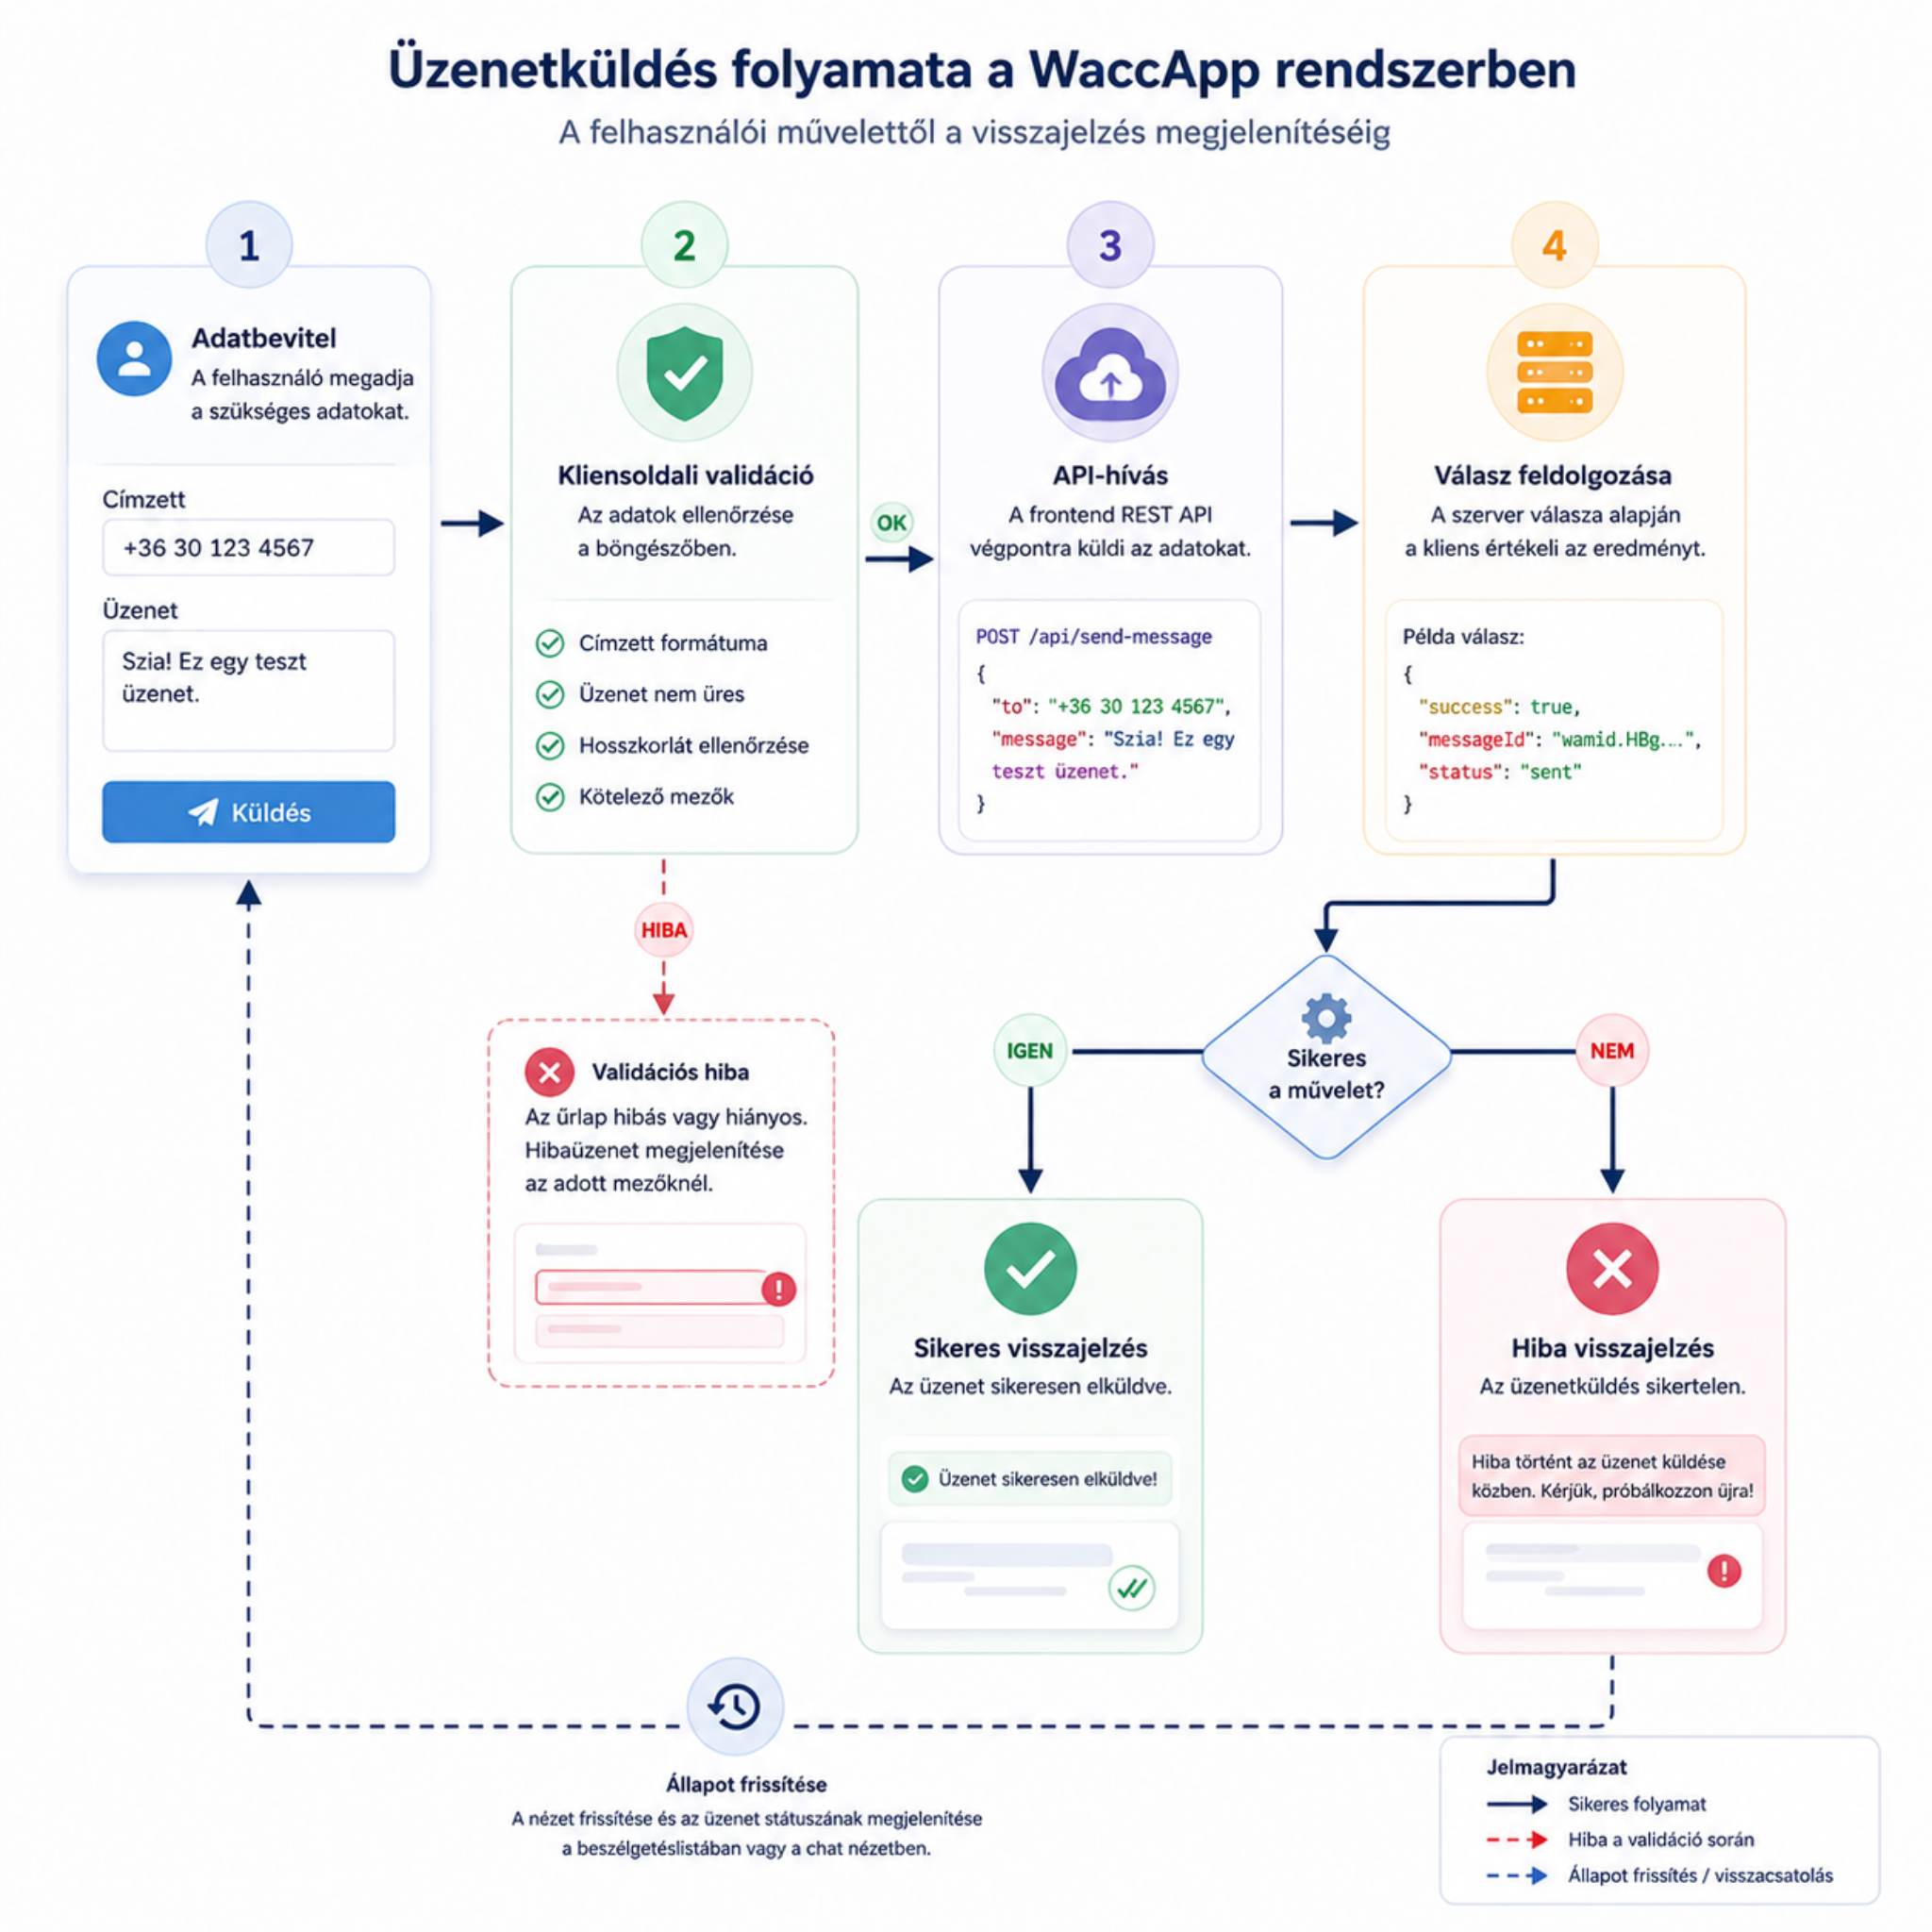
\includegraphics[width=0.92\textwidth]{images/waccapp-uezenetkuldes-folyamata.png}
    \caption{Az üzenetküldés tervezett frontendfolyamata a WaccApp rendszerben.}
    \label{fig:uzenetkuldes-folyamata}
\end{figure}

Az adatáramlási logikát az \ref{fig:uzenetkuldes-folyamata}. ábra szemlélteti. Az ábra a frontend szempontjából fontos folyamatot mutatja be, vagyis azt, amit a felhasználó közvetlenül érzékel. A validációs ág azért szerepel külön, mert hibás vagy hiányos adat esetén a kérésnek nem célszerű eljutnia a szerveroldali feldolgozásig. Sikeres válasz esetén a felület visszajelzést ad, hiba esetén pedig javítható állapotot jelenít meg. Ez a folyamat később a sablonos küldésnél, a médiaküldésnél és az időzített műveleteknél is hasonló alaplogikára épül, csak az adatcsomag és az ellenőrzések köre bővül.

\section{Validációs és hibakezelési tervezés}

A validáció tervezésekor abból kellett kiindulni, hogy a WaccApp több olyan műveletet kezel, ahol egy hiányzó vagy hibás adat a teljes kommunikáció sikertelenségét okozhatja. A validáció célja ezért nem pusztán formai ellenőrzés volt, hanem a nyilvánvalóan hibás kérések megelőzése.

Az \path{index.html} esetében a validáció első szintje a kötelező mezők ellenőrzése. Egyedi üzenetküldésnél szükséges a címzett és az üzenetszöveg. Sablonos küldésnél ellenőrizni kell a sablon kiválasztását és a paramétereket. Médiafájl küldésekor vizsgálni kell, hogy a felhasználó választott-e fájlt. Időzített küldésnél pedig az időpont értelmezhetősége is fontos, mert egy hibás időpont később sikertelen művelethez vezethet.

A kérdőívszerkesztő nézeteknél a validáció nemcsak mezőszintű, hanem logikai jellegű is. Itt nem elegendő azt ellenőrizni, hogy egy kérdés vagy válaszmező ki van-e töltve. Azt is figyelni kell, hogy a válaszokhoz tartozik-e következő kérdés vagy lezárás. Ha ez hiányzik, akkor a kérdőív futás közben megszakadhat.

A \path{filter.html} validációja az értelmezhető keresési feltételeket védi. A dátumintervallum esetében például ellenőrizni kell, hogy a kezdődátum ne legyen későbbi, mint a záródátum. A név és telefonszám kapcsolatánál pedig arra kell figyelni, hogy a felhasználó ne hozzon létre félrevezető párosítást. Egy hibás szűrés nem feltétlenül okoz technikai hibát, de rossz következtetéshez vezethet.

A hibakezelés tervezésénél alapelv volt, hogy a hibaüzenet ne csak megállítsa a folyamatot, hanem segítse a javítást. A felhasználó számára hasznosabb, ha a felület konkrétan jelzi, hogy hiányzik a címzett, üres az üzenetszöveg, nincs kiválasztott fájl, hibás az időpont vagy hiányos a kérdőív egyik kapcsolata. Így a felhasználó nem találgat, hanem célzottan tudja javítani az adatot.

Fontos tervezési szempont volt az is, hogy a frontend és a backend felelőssége elkülönüljön. A frontend képes felismerni a hiányzó mezőket és bizonyos formai hibákat, de nem döntheti el véglegesen, hogy egy telefonszám valóban elérhető-e WhatsAppon, vagy hogy a külső platform elfogadja-e az adott műveletet. A kliensoldal feladata ezért az előszűrés és a szerverválaszok érthető megjelenítése.

\section{Állapotkezelési tervezés}

A WaccApp több művelete aszinkron módon működik, ezért a frontend tervezésekor külön figyelmet kellett fordítani az állapotkezelésre. Egy üzenetküldés, fájlfeltöltés, szűrés, beszélgetésbetöltés vagy kérdőívmentés nem mindig ad azonnali eredményt. A felhasználónak mégis érzékelnie kell, hogy a művelet elindult, folyamatban van, sikeresen lezárult vagy hibára futott.

A tervezett állapotmodell négy alaphelyzetre épült. Nyugalmi állapotban a felület használatra kész. Feldolgozás alatti állapotban a kérés már elindult, de az eredmény még nem ismert. Sikeres állapotban a rendszer visszajelzi, hogy a művelet rendben lezárult. Hibás állapotban pedig a felület jelzi, hogy a folyamat nem sikerült, és lehetőség szerint megmutatja a hiba okát is.

Az \path{index.html} esetében ez főként a küldési műveleteknél fontos. Ha a felhasználó elküld egy üzenetet, sablont vagy médiafájlt, a felületnek jeleznie kell, hogy a rendszer feldolgozza a kérést. Enélkül a felhasználó könnyen újra megnyomhatja a gombot, vagy azt hiheti, hogy a rendszer nem reagált.

A \path{filter.html} esetében az állapotkezelés az adatbetöltés és az eredmények értelmezése miatt lényeges. A keresés eredménye lehet találati lista, de lehet üres eredmény is. A kettő között felhasználói szempontból fontos különbség van: az üres eredmény nem ugyanaz, mint a sikertelen lekérdezés.

A \path{conv.html} beszélgetésnézetben az állapotkezelés célja az, hogy a beszélgetés betöltése ne tűnjön bizonytalannak. Ha nincs megjeleníthető kommunikációs előzmény, azt másként kell kezelni, mint amikor az adatok betöltése hibára futott. Ez segít abban, hogy a felhasználó ne rendszerhibaként értelmezzen egy üres beszélgetést.

Az időzített küldéseknél az állapotkezelés kiterjedtebb, mert a művelet rögzítése és tényleges végrehajtása időben elválik egymástól. A felhasználónak először azt kell látnia, hogy az ütemezés mentése sikerült-e, később pedig azt, hogy a művelet várakozó, sikeres vagy sikertelen állapotban van-e. Emiatt az időzítés nem egyszerű dátummezőként, hanem állapotokkal rendelkező kommunikációs folyamatként jelent meg a tervezésben.

\section{A tervezési folyamat összegzése}

A WaccApp frontendjének tervezése során a legfontosabb cél az volt, hogy a WhatsApp Business API-ra épülő összetett kommunikációs működés a felhasználó számára kezelhető webes folyamatokká alakuljon. A tervezés nemcsak a felület vizuális kialakításáról szólt, hanem a fő felhasználói folyamatok, a nézetek felelőssége, az adatáramlás, a validáció, a hibakezelés és az állapotjelzések meghatározásáról is.

A többnézetes frontend kialakítása azért bizonyult megfelelő döntésnek, mert a rendszer fő funkciói eltérő felhasználói helyzeteket képviselnek. Az \path{index.html} a küldési műveletekre, a \path{conv.html} a beszélgetések megjelenítésére, a \path{filter.html} a visszakeresésre, a \path{questionnaire.html} és a \path{template.html} pedig a kérdőíves és sablonos folyamatokra koncentrál. Ez a bontás egyszerre teszi átláthatóbbá a használatot és könnyebben karbantarthatóvá a fejlesztést.

A tervezési folyamat másik fontos eredménye az egységes működési minta kialakítása volt. A fő folyamatok eltérő célt szolgálnak, de alaplogikájuk hasonló: a felhasználó adatot ad meg, a frontend ellenőriz, API-kérést indít, majd a válasz alapján frissíti a felületet. Ez az ismétlődő minta biztosítja, hogy a WaccApp több HTML-nézetből állva is egységes frontendként működjön.

\chapter{Felhasználói élmény és reszponzív dizájn}

Az előző fejezet a WaccApp frontendjének tervezési folyamatát mutatta be: milyen felhasználói folyamatokból, nézetekre bontási döntésekből, adatáramlási elvekből, validációs és állapotkezelési szempontokból épült fel a rendszer. Ebben a fejezetben már az kerül előtérbe, hogy ezek a tervezési döntések hogyan jelennek meg a felhasználói élményben és a reszponzív működésben.

A WaccApp felületének használhatósága azon múlik, hogy a felhasználó mennyire gyorsan érti meg az adott nézet célját, mennyire egyértelmű számára a következő lépés, és kap-e időben visszajelzést a hibás vagy sikeres műveletekről. A UX-fejezet ezért nem újra a szerkezeti döntéseket tárgyalja, hanem azt vizsgálja, hogyan segítik ezek a döntések a mindennapi használatot: az adatbevitelt, a hibajavítást, a beszélgetések olvasását, a szűrést és a kisebb kijelzőn történő kezelést.

\section{Felületi szervezés és információs hierarchia}

A WaccApp felületi szervezésénél az volt a legfontosabb, hogy a felhasználó az adott oldalon gyorsan felismerje, mi a következő értelmes lépés. Egy kommunikációs rendszerben különösen zavaró, ha a felület egyszerre túl sok lehetőséget mutat, de nem derül ki, melyik művelethez melyik mező tartozik. Ezért minden fő nézetnek saját hangsúlyt kellett kapnia.

Az \path{index.html} oldalon a felhasználó küldési folyamatot indít. Itt a címzett, a küldési mód, a tartalom és az indítási lehetőség kerül előtérbe. A felületnek azt kell támogatnia, hogy a felhasználó először kiválassza, milyen típusú kommunikációt szeretne indítani, majd ehhez igazodva adja meg a szükséges adatokat. Egy szöveges üzenetnél a címzett és az üzenettartalom a fontos, sablonos küldésnél viszont már a sablon és a paraméterek is szerepet kapnak. Ha ezeket a mezőket a felület nem választaná el egymástól egyértelműen, a használat könnyen bizonytalanná válna.

A \path{filter.html} egészen más logikát követ. Itt a felhasználó nem új kommunikációt indít, hanem korábbi adatok között keres. Emiatt ezen az oldalon a szűrési feltételek sorrendje és értelmezhetősége fontosabb, mint egy nagy, látványos műveleti gomb. A név, telefonszám, üzenettípus, dátumintervallum vagy kérdőív szerinti keresés akkor használható jól, ha a felület nem egyszerűen egymás alá helyezi a mezőket, hanem segít abban, hogy a felhasználó értelmes keresési feltételt állítson össze.

A kérdőívszerkesztő oldalaknál a legnagyobb kihívást az jelentette, hogy a felhasználó nem egyetlen adatot ad meg, hanem egymással összefüggő elemeket épít fel. Egy kérdéshez válaszok tartozhatnak, a válaszokhoz pedig következő lépések kapcsolódhatnak. Ilyen helyzetben a felületnek nem elég szép beviteli mezőket adnia. Segítenie kell abban is, hogy a szerkesztés közben a folyamat logikája követhető maradjon. Ha a kérdés, a válasz és a következő lépés vizuálisan túl távol kerül egymástól, a felhasználó könnyebben hibázik.

A \path{conv.html} beszélgetésnézete szintén külön felületi szervezést igényel. Itt nem az adatbevitel az elsődleges, hanem az időrendben megjelenő kommunikáció értelmezése. A bejövő és kimenő üzenetek elkülönítése, az időpontok követhetősége és a médiaelemek megjelenítése mind azt szolgálja, hogy a felhasználó ne nyers adatsorokat lásson, hanem egy beszélgetési folyamatot. Ez a nézet akkor működik jól, ha a felhasználó gyorsan megérti, ki küldött üzenetet, mikor történt a küldés, és milyen tartalom kapcsolódott az adott kommunikációhoz.

\section{Reszponzív működés és képernyőmérethez igazított felület}

A WaccApp reszponzív kialakításánál nem az volt a cél, hogy az asztali nézet egyszerűen kisebb méretben jelenjen meg mobilon. Egy kisebb kijelzőn másképp használja az ember a rendszert. Kevesebb információ fér el egyszerre, az érintéses vezérlés miatt nagyobb szerepet kapnak a gombméretek, és a túl hosszú űrlapok gyorsabban fárasztóvá válnak. Emiatt a reszponzív működés nem pusztán formai kérdés volt, hanem közvetlenül befolyásolta a használhatóságot.

Az \path{index.html} esetében mobilon különösen fontos, hogy a felhasználó ne vesszen el a különböző küldési lehetőségek között. Ha az üzenetküldés, sablonküldés, kérdőívindítás, médiaküldés és időzítés egyszerre túl nagy hangsúlyt kapna, a felület zsúfolttá válna. A használhatóság szempontjából ezért az volt a lényeges, hogy a kiválasztott művelethez kapcsolódó mezők kerüljenek előtérbe, és a felhasználó ne érezze úgy, hogy minden küldési módot egyszerre kell értelmeznie.

A \path{conv.html} oldalon a reszponzív működés még érzékenyebb kérdés. Egy beszélgetésnézet akkor használható jól, ha a tényleges üzenetfolyam kapja a legtöbb helyet. Kisebb kijelzőn a túl magas fejléc, a túl nagy navigációs elem vagy a sok helyet elfoglaló alsó sáv könnyen elveszi a teret attól, ami miatt a felhasználó megnyitotta az oldalt: a beszélgetés áttekintésétől. Ezért ebben a nézetben a reszponzív tervezés lényege az volt, hogy a chat-szerű élmény kisebb képernyőn se essen szét, az üzenetek pedig görgethető, olvasható formában maradjanak.

A beszélgetésnézet fejlesztése közben különösen jól látszott, hogy egy apró elrendezési döntés is erősen befolyásolja a használhatóságot. Amikor a fejléc vagy az üzenetküldő sáv túl nagy helyet foglalt el, a tényleges beszélgetési terület szűknek és nehezen használhatónak hatott. Emiatt a \path{conv.html} esetében törekedtem arra, hogy a fejléc és az alsó beviteli rész minél visszafogottabb legyen, a fő hangsúly pedig az üzenetfolyamon maradjon.

A \path{filter.html} esetében más probléma jelentkezik. A szűrési felület több mezőt is tartalmazhat, és ezek asztali nézetben még kényelmesen áttekinthetők. Mobilon viszont ugyanaz a mezőmennyiség gyorsan túl hosszúvá vagy nehezen kezelhetővé válhat. Ezért a szűrésnél fontosabbá vált a mezők logikus sorrendje és a fokozatos kitöltés lehetősége. A felhasználó először megadhatja a legfontosabb feltételeket, majd az eredményeket külön blokkban értelmezheti. Ez kevésbé látványos megoldás, mint egy mindent egyszerre mutató felület, de használat közben biztonságosabb.

A kérdőívszerkesztő oldalaknál a reszponzivitás azért volt különösen nehéz, mert a kérdések, válaszok és elágazások egymással kapcsolatban állnak. Asztali nézetben ezek az összefüggések könnyebben áttekinthetők, mobilon viszont gyorsan elveszhet a kapcsolat a kérdés és a hozzá tartozó válaszlogika között. Emiatt ezeknél az oldalaknál nem az volt a cél, hogy minden elem egyszerre látható maradjon, hanem az, hogy a szerkesztés egymás után követhető blokkokra bontva is érthető legyen. [R6], [R7], [R9]

\section{Validációs döntések és hibamegelőzés}

A validáció a WaccApp-ban nem önálló technikai extra, hanem a felhasználói élmény egyik alapja. A rendszer több olyan műveletet kezel, ahol egy hiányzó vagy hibás adat később sikertelen küldést, megszakadó kérdőívet vagy értelmezhetetlen szűrést okozhat. Emiatt a frontendnek már a művelet elindítása előtt jeleznie kell a nyilvánvaló problémákat.

Az \path{index.html} oldalon ez leginkább a küldési módok közötti különbségnél jelenik meg. Egy egyszerű szöveges üzenetnél a címzett és az üzenettartalom megléte a legfontosabb. Sablonos küldésnél már a sablon kiválasztása és a paraméterek kitöltése is szükséges. Médiafájl esetén a kiválasztott állomány megléte és típusa kerül előtérbe, időzített küldésnél pedig az is számít, hogy az időpont értelmezhető-e. A felületnek ezért nem általános hibát kell adnia, hanem az adott művelethez kapcsolódó problémát kell megmutatnia. [R14]

A kérdőívszerkesztő felületeken a validáció már nemcsak mezőszintű kérdés. Itt nem elég azt figyelni, hogy egy kérdés szövege vagy egy válaszmező ki van-e töltve. Azt is ellenőrizni kell, hogy a válaszokból kialakuló útvonal folytatható-e. Ha egy válaszhoz nem tartozik következő kérdés vagy lezárás, akkor a kérdőív futás közben megakadhat. Ez a felhasználó számára nem feltétlenül szerkesztési hibaként jelenik meg, hanem úgy, mintha a rendszer nem működne. Ezért fontos, hogy a hibás kapcsolatok lehetőleg már a szerkesztéskor láthatóvá váljanak.

A \path{filter.html} esetében a validáció más jellegű. Itt nem küldési hibát kell megelőzni, hanem azt, hogy a felhasználó értelmetlen vagy félrevezető keresést indítson. A dátumintervallum például csak akkor értelmezhető, ha a kezdő és záró dátum logikus sorrendben van. A név és telefonszám kapcsolata szintén érzékeny pont, mert egy rossz párosítás hibás következtetéshez vezethet. A szűrőfelület validációja ezért nemcsak technikai ellenőrzés, hanem az eredmények értelmezhetőségét is védi.

A hibamegelőzésnél fontos volt, hogy a felület ne büntesse a felhasználót. Egy hibaüzenet akkor jó, ha segít javítani, nem pedig csak megállítja a folyamatot. A WaccApp-ban ezért a validáció célja az volt, hogy a felhasználó minél hamarabb lássa, mit kell pótolnia vagy módosítania. Egy hiányzó telefonszám, üres üzenet, rosszul beállított időpont vagy félbehagyott kérdőívkapcsolat esetén jobb azonnal visszajelzést adni, mint megvárni, amíg a backend vagy a külső platform utasítja vissza a kérést. [R13], [R14]

\section{Állapotjelzések és visszacsatolási logika}

A WaccApp több művelete aszinkron módon működik, ezért a felhasználó nem mindig kap azonnali tartalmi eredményt. Egy üzenetküldés, fájlfeltöltés, szűrés vagy beszélgetésbetöltés közben a háttérben kérés indul a backend felé, majd a válasz alapján frissül a felület. Ha ilyenkor semmilyen jelzés nem jelenik meg, a felhasználó könnyen azt hiheti, hogy nem történt semmi, és újra megnyomja a gombot, vagy megszakítottnak gondolja a műveletet.

Az üzenetküldésnél ez különösen fontos. A küldés gomb megnyomása után a felhasználónak rövid időn belül érzékelnie kell, hogy a rendszer feldolgozza a kérést. Nem kell bonyolult animáció vagy túlmagyarázott üzenet, de valamilyen állapotjelzés szükséges. Egy státuszszöveg, módosított gombállapot vagy rövid visszajelzés már elég lehet ahhoz, hogy a felhasználó tudja, hogy a kattintása nem veszett el.

A szűrésnél és a beszélgetésbetöltésnél a visszacsatolás más szerepet kap. Itt nem az a fő kérdés, hogy egy üzenet sikeresen elment-e, hanem az, hogy az adatok frissültek-e. A \path{filter.html} esetében a felhasználónak tudnia kell, hogy a keresés lefutott, akkor is, ha nincs találat. Egy üres eredménylista önmagában félreérthető lehet, mert nem derül ki belőle, hogy nincs adat, vagy a lekérdezés nem működött. A \path{conv.html} esetében hasonló a helyzet: ha a beszélgetés betöltése közben a felület üresnek látszik, az könnyen rendszerhibának tűnhet.

A médiafájloknál a visszajelzés azért kap nagyobb szerepet, mert a fájlküldés általában lassabb és érzékenyebb folyamat, mint egy egyszerű szöveg elküldése. A felhasználó először kiválaszt egy fájlt, majd várja, hogy az valóban feldolgozásra és küldésre kerüljön. Ilyenkor a felületnek nemcsak a végeredményt kell jeleznie, hanem azt is, hogy a rendszer dolgozik. Ellenkező esetben könnyen előfordulhat, hogy a felhasználó újra kiválasztja a fájlt vagy ismételten elindítja a küldést.

Az időzített műveleteknél a visszacsatolás még összetettebb, mert a művelet rögzítése és tényleges végrehajtása időben elválik egymástól. A felhasználó először azt várja, hogy a rendszer elfogadta-e az ütemezést, később pedig azt szeretné látni, hogy az adott küldés várakozik, sikeresen lefutott vagy hibára futott. Ezek az állapotok nem pusztán technikai információk, hanem a felhasználói kontroll részei. A WaccApp-ban ezért az állapotjelzés nem dekorációként jelenik meg, hanem a kommunikációs folyamat értelmezését segíti. [R13], [R14]

\section{Vizuális következetesség és alap hozzáférhetőség}

A WaccApp több különálló HTML-nézetből áll, ezért a vizuális következetesség különösen fontos volt. Ha minden oldal más gombhasználatot, más hibaüzenet-megjelenítést és más űrlaplogikát követne, a felhasználó minden nézetnél újra tanulná a rendszert. Ez nemcsak kényelmetlen lenne, hanem hibákhoz is vezethetne, főleg olyan műveleteknél, ahol üzenetküldésről, fájlcsatolásról vagy kérdőívindításról van szó.

A következetesség ugyanakkor nem azt jelenti, hogy minden oldalnak ugyanúgy kell kinéznie. Az \path{index.html}, a \path{conv.html}, a \path{filter.html} és a kérdőívszerkesztő oldalak más feladatot látnak el, ezért természetes, hogy az elrendezésük is eltér. A fontos az volt, hogy az azonos típusú elemek hasonló jelentést hordozzanak. Egy elsődleges műveleti gomb mindenhol fő cselekvést indítson, a hibaüzenetek a javítandó adatra irányítsák a figyelmet, a státuszjelzések pedig a folyamat aktuális állapotát mutassák.

Az alapvető hozzáférhetőségi szempontok a WaccApp-ban főként a mindennapi használhatóságot támogatták. A jól olvasható szöveg, a megfelelő kontraszt, a látható fókuszállapot és a kényelmesen használható gombméret nem látványos fejlesztési eredmény, mégis sokat számít. Egy túl kicsi gomb mobilon könnyen félrekoppintáshoz vezethet, egy gyenge kontrasztú hibaüzenet pedig pont akkor nem segít, amikor a felhasználónak szüksége lenne rá.

A rendszer nem teljes körű akadálymentesítési projektként készült, de a legfontosabb alapelveket figyelembe kellett venni. A felületnek olvashatónak, kezelhetőnek és érthetőnek kell maradnia akkor is, ha a felhasználó kisebb kijelzőn dolgozik, gyorsan akar üzenetet küldeni, vagy egy hosszabb kérdőíves szerkesztési folyamatban navigál. Ezek az apró döntések együtt határozzák meg, hogy a rendszer mennyire használható a gyakorlatban. [R6], [R7]

\section{A UX-döntések szerepe a WaccApp használhatóságában}

A WaccApp felhasználói élményét nem egyetlen látványos megoldás határozza meg, hanem sok kisebb döntés együttese. A többnézetes felépítés segít elkülöníteni a különböző feladatokat, a reszponzív működés használhatóbbá teszi a rendszert eltérő kijelzőméreteken, a validáció csökkenti a hibás műveleteket, az állapotjelzések pedig láthatóvá teszik a háttérben futó folyamatokat. Ezek együtt adják azt az élményt, hogy a felhasználó nem technikai akadályokkal, hanem kezelhető munkafolyamatokkal találkozik.

A fejezetben bemutatott döntések a korábbi fejezet követelményeire épülnek. Itt a kérdés az, hogy ezek a funkciók hogyan váltak használható felületi megoldássá. A küldési felületnél ez a megfelelő mezősorrendben és visszajelzésben jelenik meg. A beszélgetésnézetnél az időrendi és vizuálisan elkülönített megjelenítésben. A szűrésnél a feltételek kezelhető szervezésében. A kérdőívszerkesztésnél pedig abban, hogy a kérdések és válaszok kapcsolatai követhetők maradjanak. A WaccApp használhatósága tehát azon múlik, hogy a felhasználó mennyire tudja magabiztosan végig vinni a fő műveleteket. Ha érti, mit kell kitöltenie, látja, ha valami hiányzik, kap visszajelzést a folyamat állapotáról, és a különböző nézetek között váltva sem veszti el a rendszer logikáját, akkor a frontend teljesíti a szerepét. [R9], [R13], [R14]

\chapter{A WaccApp frontend architektúrája és mappaszerkezete}

A korábbi fejezetek bemutatták, hogy a WaccApp frontendje több, egymást kiegészítő felhasználói folyamat köré szerveződik. Ebben a fejezetben már nem a tervezési indoklás vagy a használhatósági háttér áll a középpontban, hanem a konkrét frontendarchitektúra: mely nézetekből, fájlokból és mappákból épül fel a rendszer, és ezek hogyan kapcsolódnak egymáshoz.

A fejezet célja annak bemutatása, hogy a WaccApp saját fájlszerkezete és nézetrendszere hogyan támogatja a megvalósított funkciókat. Itt kap helyet a fő HTML-nézetek felelőssége, a kliensoldali adatáramlás konkrétabb értelmezése, a nézetek közötti kapcsolat, valamint a frontend szempontból fontos mappák és állományok szerepe.

\section{A többnézetes frontend szervezési logikája}

A WaccApp frontendje több belépőpontos webes felületként épül fel. A gyakorlatban ez azt jelenti, hogy a fő funkciók külön HTML-oldalakhoz kapcsolódnak, de közös kommunikációs adatokat, hasonló felületi mintákat és azonos backendkapcsolatokat használnak. Ebben a fejezetben a hangsúly már nem a többnézetes döntés indoklásán, hanem az egyes nézetek felelősségi körén és kapcsolódásán van.

A többnézetes szervezés ezért a WaccApp-ban nem az oldalak véletlenszerű szétválasztását jelenti, hanem a feladatok felelősségi körök szerinti elkülönítését. Az \path{index.html} a küldési műveletek központi indítófelületeként működik. A kommunikáció visszakövetését a \path{messages.html}, a \path{sent-messages.html} és a \path{conv.html} támogatja. A kérdőíves és sablonos szerkesztési feladatok a \path{questionnaire.html}, a \path{template.html}, a \path{template-menu.html} és a \path{template-single.html} oldalakhoz kapcsolódnak. A \path{filter.html} önálló elemző és visszakereső nézetként jelenik meg, míg a \path{login.html}, a \path{menu.html}, az \path{admin.html}, az \path{account.html} és a \path{privacy.html} a hozzáféréshez, navigációhoz, adminisztrációhoz és tájékoztatáshoz kötődő feladatokat fedik le. 

Ez a szervezési logika azért előnyös, mert minden oldal egy elsődleges feladatra koncentrálhat. Az \path{index.html} nem terhelődik túl részletes statisztikai vagy adminisztratív elemekkel, mert ezek más nézetek felelősségi körébe tartoznak. A \path{filter.html} nem küldési felületként működik, hanem a már létrejött kommunikációs adatok értelmezésére szolgál. A \path{conv.html} nem általános üzenetlista, hanem egy adott kontakthoz kapcsolódó beszélgetés követését támogatja. Így a frontend szerkezete nemcsak fejlesztői oldalról válik átláthatóbbá, hanem a felhasználó számára is könnyebben tanulható rendszert eredményez. 

A WaccApp ebben az értelemben nem klasszikus egyoldalas alkalmazásként működik, de nem is egyszerű, egymástól elszigetelt HTML-oldalak gyűjteménye. Az egyes nézetek közös backendkapcsolatokon, azonos kommunikációs adatokon és hasonló felhasználói mintákon keresztül kapcsolódnak egymáshoz. A rendszer szerkezeti logikája tehát az elkülönítés és az összekapcsolás egyensúlyára épül. 

\section{A fő frontend nézetek felelőssége}

A WaccApp frontendjének egyik legfontosabb nézete az \path{index.html}, amely a kommunikációs műveletek központi indítófelülete. Ezen az oldalon találkozik a felhasználó azokkal a fő műveletekkel, amelyekkel üzenetet, sablont, kérdőívet vagy médiafájlt küldhet, illetve időzített küldést állíthat be. Az oldal felelőssége ezért nem egyszerűen egy üzenetmező megjelenítése, hanem több küldési mód egy felületen belüli kezelése. A frontendnek ebben a nézetben a választott művelethez igazodva kell kezelnie a beviteli mezőket, a szükséges adatokat és a művelet indítását. 

A \path{messages.html} és a \path{sent-messages.html} a kommunikációs események listaalapú visszakövetését támogatják. A két nézet szerepe abban különíthető el, hogy a beérkező és az elküldött tartalmak nem keverednek egyetlen túlterhelt listába, hanem célzottan áttekinthetők. Ez a felosztás akkor válik különösen hasznossá, amikor a felhasználó nem egy konkrét beszélgetést szeretne megnyitni, hanem gyorsan ellenőrizni akarja, milyen üzenetek érkeztek be, vagy milyen tartalmak kerültek korábban elküldésre. 

A \path{conv.html} a kommunikáció részletesebb értelmezésére szolgál. Ez a nézet egy adott kontakthoz kapcsolódó beszélgetésfolyamot jelenít meg, ezért más felületi logikát igényel, mint egy egyszerű listaoldal. A beszélgetésnézetben az időrendiség, a bejövő és kimenő üzenetek elkülönítése, valamint a szöveges és médiás tartalmak értelmezhető megjelenítése kerül előtérbe. A \path{conv.html} jelentősége abban áll, hogy a korábbi kommunikációt nem darabokra bontott adatsorként, hanem folyamatként mutatja meg. 

A \path{filter.html} a visszakeresés és az alapvető értelmezés nézete. Ez az oldal nem új kommunikációs műveletet indít, hanem a már meglévő adatokból segít célzott eredményeket előállítani. A felhasználó név, telefonszám, üzenettípus, dátumintervallum, kérdőív vagy válasz alapján szűrhet, ezért a nézet felelőssége túlmutat egy egyszerű keresőmezőn. A \path{filter.html} feladata az, hogy a több feltételből álló keresést kezelhető formába rendezze, és az eredményeket a felhasználó számára áttekinthetően jelenítse meg. 

A kérdőíves működéshez két eltérő logikájú szerkesztői irány kapcsolódik. A \path{questionnaire.html} a szöveges vagy számalapú válaszokra épülő kérdőívek kezelését támogatja, ahol a kérdések, válaszok és elágazások szerkesztése a fő feladat. Ezzel szemben a \path{template.html}, a \path{template-menu.html} és a \path{template-single.html} a sablonos, gombos kommunikációhoz kapcsolódó szerkesztési felületeket adják. A \path{template-menu.html} navigációs szerepet kap a sablonos feladatok között, a \path{template-single.html} az egyszerűbb sablonkészítési folyamatot támogatja, míg a \path{template.html} az összetettebb, több lépésből álló sablonos kérdőívlogika szerkesztéséhez kapcsolódik. 

A belépési és kiegészítő nézetek szintén a frontend egészének részei, de más szerepet töltenek be, mint a kommunikációs modulok. A \path{login.html} a belépési folyamatot biztosítja, a \path{menu.html} a főbb oldalak közötti navigációt segíti, az \path{admin.html} az adminisztratív feladatokhoz kapcsolódik, az \path{account.html} a felhasználói fiókhoz tartozó beállítások nézete, a \path{privacy.html} pedig az adatvédelmi tájékoztatás megjelenítését szolgálja. 

\section{Kliensoldali adatáramlás}

A WaccApp kliensoldali adatáramlása a nézetek eltérő szerepe ellenére következetes működési elvet követ. A frontend minden jelentős műveletnél a felhasználói bevitelt alakítja olyan adattá, amelyet a háttérrendszer értelmezni tud. A korábbi fejezetekben ez általános működési modellként jelent meg, ebben a fejezetben azonban a hangsúly azon van, hogy ez a gyakorlatban hogyan jelenik meg a WaccApp fő nézeteiben. 

Az üzenetküldés esetében az adatáramlás az \path{index.html} oldalon indul. A felhasználó megadja a címzettet, kiválasztja a küldési módot, majd kitölti az adott típushoz szükséges adatokat. Egyszerű szöveges üzenetnél ez elsősorban a telefonszámot és az üzenettartalmat jelenti. Sablonos küldésnél a sablon neve, a kapcsolódó paraméterek és a nyelvi beállítások is szerepet kapnak. Médiafájl küldésekor a kiválasztott állomány is a folyamat részévé válik. A frontend a megadott adatokat a művelet típusának megfelelően dolgozza fel, majd a háttérrendszer felé továbbítja. A szerver válasza alapján az oldal nemcsak technikai választ kap, hanem a felhasználó számára értelmezhető állapotot jelenít meg. 

A kérdőívszerkesztés adatáramlása ettől eltérő jellegű, mert itt nem egyszeri küldési műveletről, hanem szerkeszthető folyamatmodellről van szó. A \path{questionnaire.html} oldalon a felhasználó kérdéseket, válaszlehetőségeket és kapcsolódásokat hoz létre. Ezek az adatok egymással összefüggő szerkezetet alkotnak, hiszen egy válasz meghatározhatja a következő kérdést. A frontend feladata ebben a helyzetben az, hogy a beírt tartalmakat és logikai kapcsolatokat olyan struktúrába rendezze, amely menthető és később újra felhasználható. A sablonos kérdőívek esetében a \path{template.html} hasonlóan folyamatot szervez, de ott a kérdések és válaszok a WhatsApp sablonos, gombos kommunikációjához igazodnak. 

A szűrési folyamat a \path{filter.html} oldalon más típusú adatáramlást használ. Itt a felhasználó nem új kommunikációs tartalmat hoz létre, hanem meglévő adatok között keres. A frontend a megadott feltételekből lekérdezési szempontokat állít össze. Ilyen feltétel lehet a név, a telefonszám, az üzenettípus, a dátumintervallum, a kérdőív vagy egy konkrét válasz. A válasz megérkezése után az oldal nem egyszerűen nyers adatokat jelenít meg, hanem az eredményeket olyan formában rendezi, hogy azok összehasonlíthatók és értelmezhetők legyenek. A \path{conv.html} esetében az adatáramlás szintén lekérdezésre épül, de ott a cél nem szűrt eredménylista, hanem egy adott kontakthoz kapcsolódó beszélgetés időrendi megjelenítése. 

Ez a három példa jól mutatja, hogy a WaccApp frontendjében az adatáramlás nem minden oldalon ugyanazt a feladatot szolgálja. Az \path{index.html} műveletet indít, a \path{questionnaire.html} és a \path{template.html} szerkeszthető kommunikációs logikát épít, a \path{filter.html} és a \path{conv.html} pedig meglévő adatok értelmezését támogatja. A közös pont az, hogy a frontend minden esetben közvetítő szerepet tölt be a felhasználó szándéka és a háttérrendszer által feldolgozható adatszerkezet között. [R10] 

\section{A nézetek közötti kapcsolódás}

A WaccApp frontendje több HTML-oldalból áll, de ezek az oldalak nem elszigetelt egységek. A rendszer használata során az egyes nézetek egymásra épülnek, és ugyanannak a kommunikációs folyamatnak különböző szakaszait támogatják. Ez a kapcsolódás adja a frontend tényleges architekturális értékét, mert az oldalak nem csupán külön funkciókat valósítanak meg, hanem együtt alkotnak használható kommunikációs környezetet. 

Az \path{index.html} több folyamat kiindulópontja. Innen indulhat egyszerű szöveges üzenet, sablonos üzenet, kérdőív, médiafájl vagy időzített küldés. A művelet eredménye később más nézetekben válik visszakövethetővé. Az elküldött tételek a \path{sent-messages.html} oldalon, a beérkező válaszok a \path{messages.html} felületen, a teljesebb kommunikációs folyamat pedig a \path{conv.html} nézetben értelmezhető. Ez a kapcsolat biztosítja, hogy a küldési művelet ne egyszeri, elszigetelt esemény legyen, hanem a kommunikációs előzmények részévé váljon. 

A kérdőíves oldalak szintén kapcsolódnak a kommunikációs és szűrési nézetekhez. A \path{questionnaire.html} és a \path{template.html} szerkesztőfelületein létrehozott kérdőívek az \path{index.html} oldalról indíthatók el, a válaszok pedig később a kommunikációs előzmények és a szűrési felület részeként értelmezhetők. Ez a folyamat különösen fontos, mert a kérdőív nem önmagában értékes, hanem akkor, ha a válaszok visszakereshetők és kiértékelhetők. A \path{filter.html} ezért a kérdőíves funkciók természetes folytatásaként is működik. 

A médiafájlok kezelése ugyancsak több nézetet kapcsol össze. A fájl kiválasztása és küldése elsősorban az \path{index.html} oldalhoz kapcsolódik, az elküldött médiafájlok tárolása és későbbi megjelenítése azonban már a public/uploads és a public/sent\_media mappákhoz, valamint a beszélgetésnézethez kötődik. A \path{conv.html} ebben a kapcsolatban azért kap fontos szerepet, mert a korábban elküldött médiatartalmakat a kommunikációs kontextus részeként jeleníti meg. Így a fájl nem pusztán egy feltöltött állomány marad, hanem a beszélgetés értelmezhető eleme lesz. 

A navigációs és kiegészítő oldalak az egész rendszer keretét adják. A \path{menu.html} a fő modulok közötti váltást támogatja, a \path{login.html} a hozzáférés kezdeti pontja, az \path{account.html} és az \path{admin.html} a felhasználói és adminisztratív beállításokhoz kapcsolódnak, a \path{privacy.html} pedig az adatkezelési tájékoztatás megjelenítését biztosítja. Ezek az oldalak nem a kommunikációs logika központi elemei, de szükségesek ahhoz, hogy a rendszer ne csak funkciók halmaza, hanem teljesebb webes alkalmazásként legyen használható. 

A nézetek közötti kapcsolatot az \ref{fig:frontend-nezetkapcsolat}. ábra foglalja össze. Az ábra célja, hogy megmutassa a WaccApp fő frontendnézeteinek szerepét és egymáshoz való viszonyát.

\begin{figure}[H]
\centering
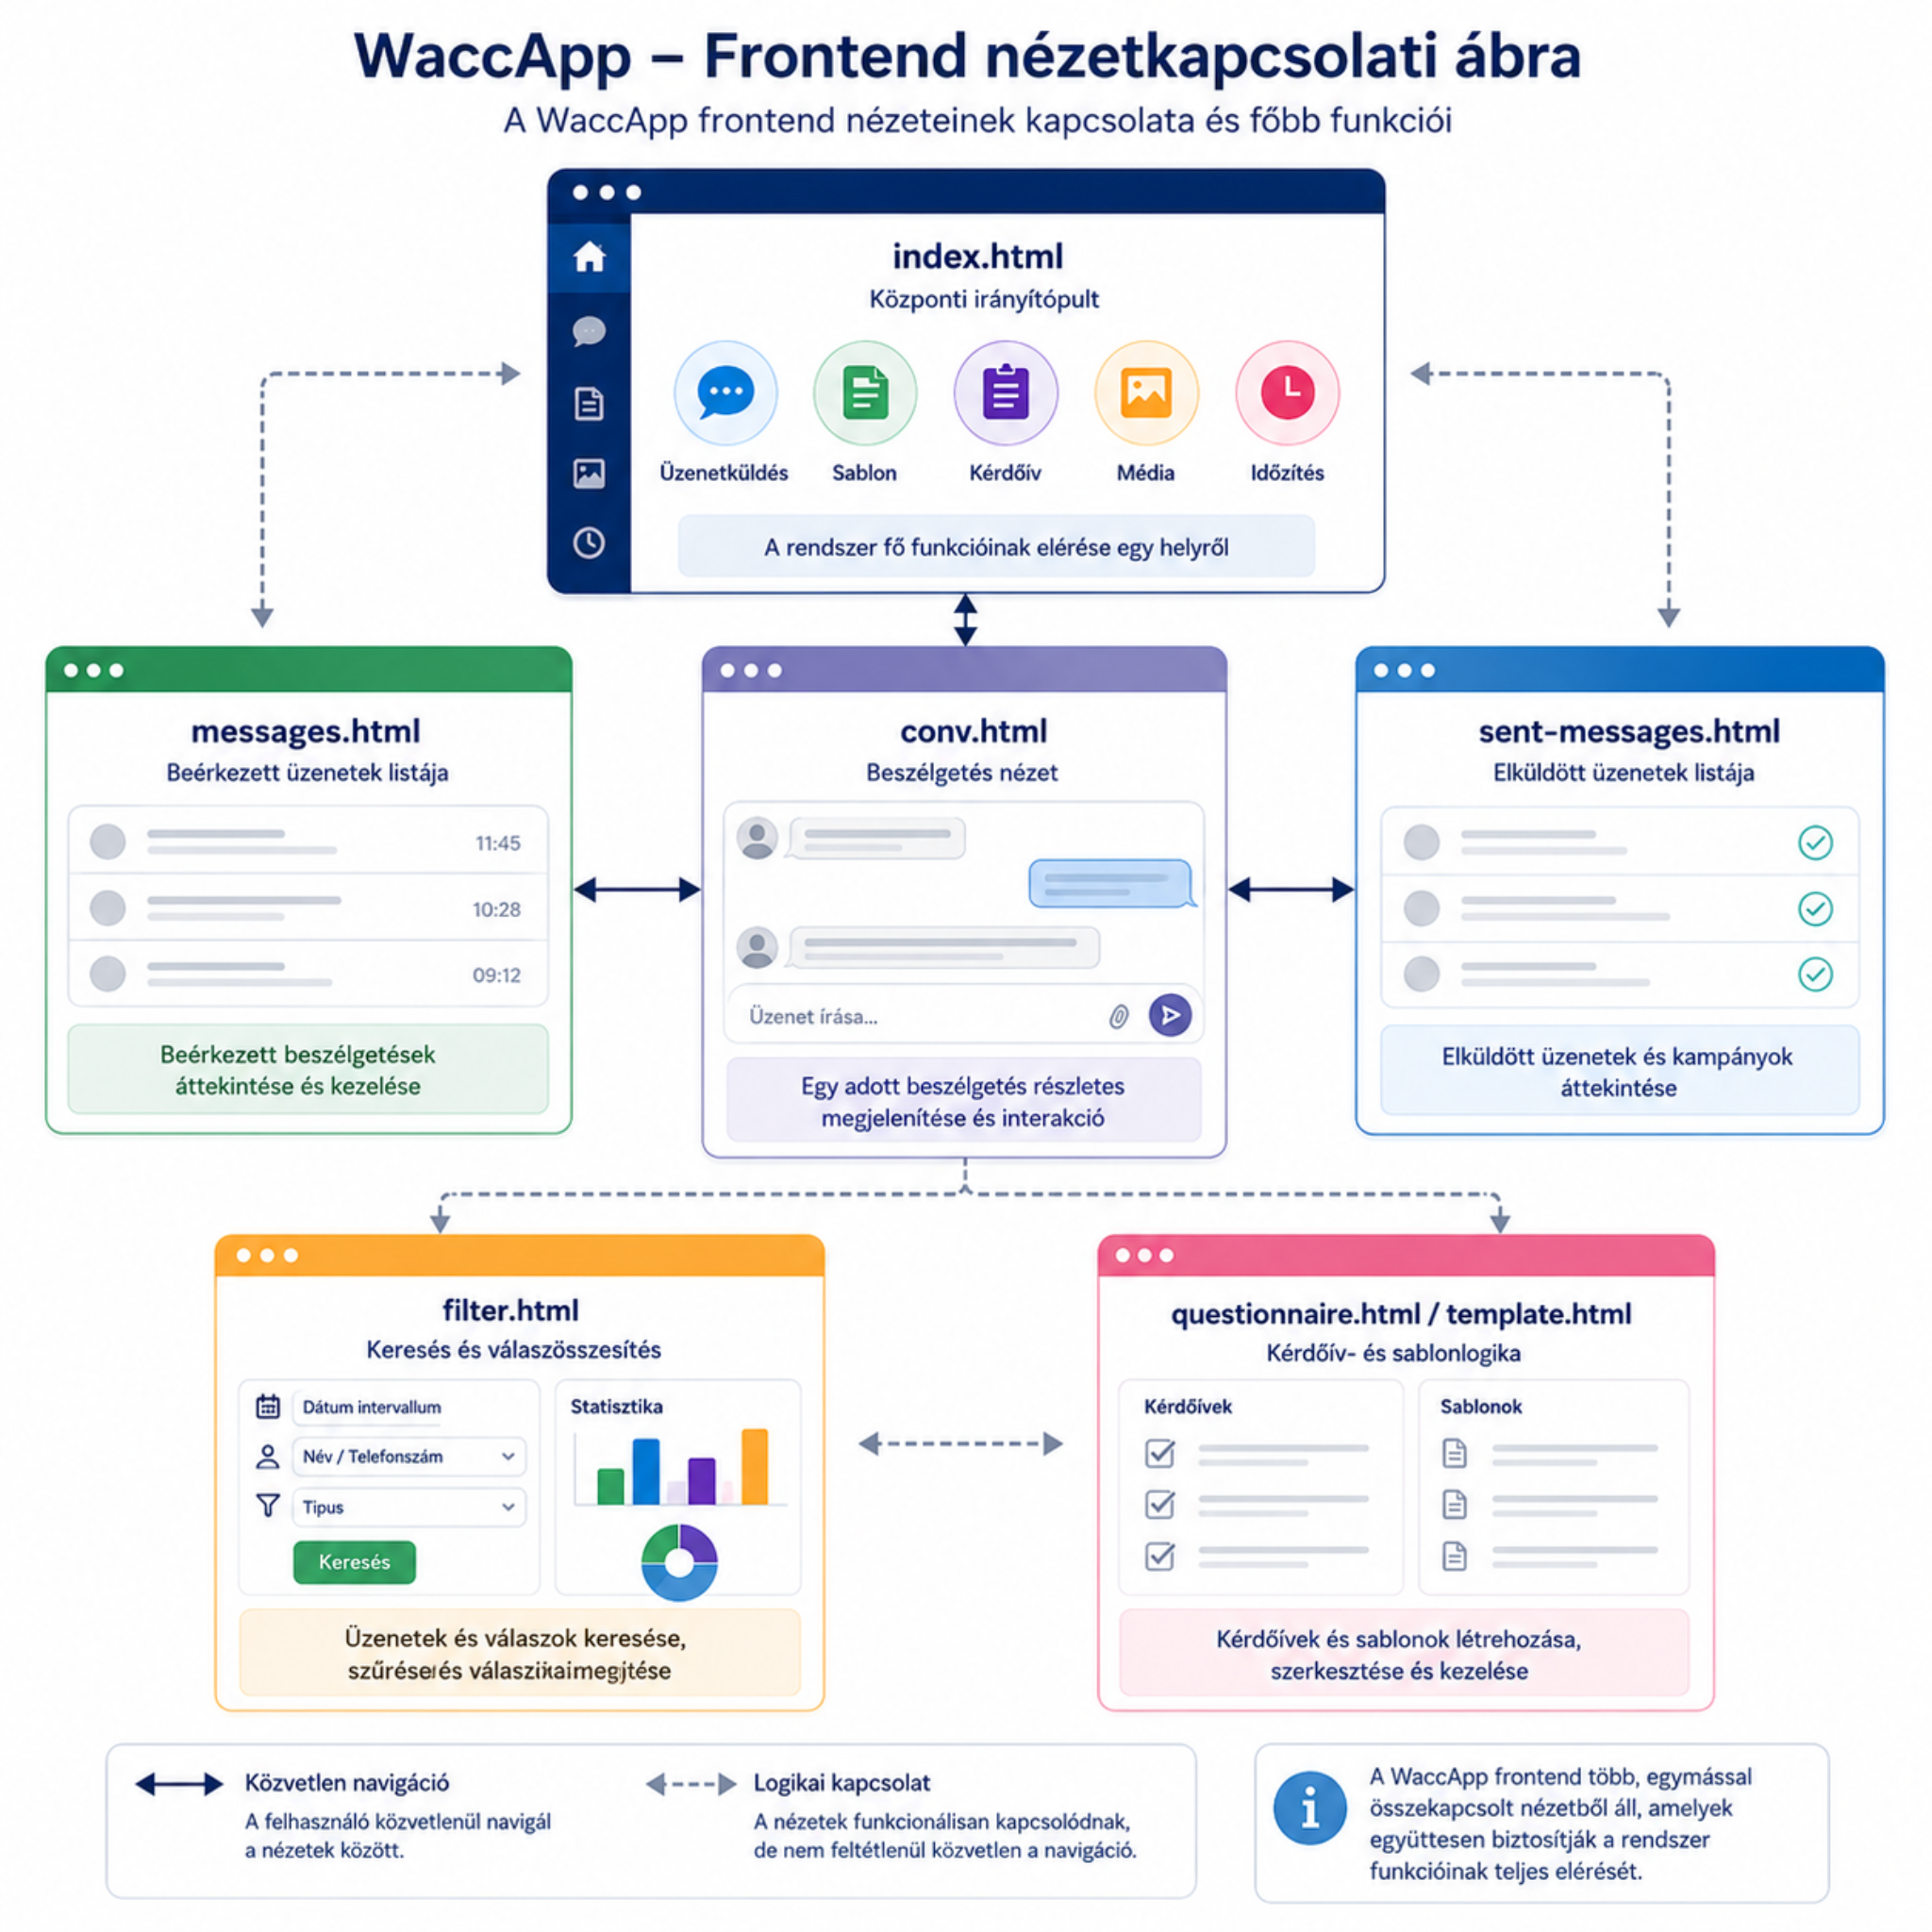
\includegraphics[width=0.95\textwidth]{images/waccapp-frontend-nezetkapcsolat.png}
\caption{A WaccApp frontend nézeteinek kapcsolata és főbb funkciói.}
\label{fig:frontend-nezetkapcsolat}
\end{figure}

Az ábrán elkülönülnek azok a nézetek, amelyek közvetlen felhasználói navigációval érhetők el, és azok a kapcsolatok, amelyek inkább funkcionális összefüggést jelentenek. Az \path{index.html} a kommunikációs műveletek indítófelülete, a \path{messages.html} és a \path{sent-messages.html} a kommunikációs események listaalapú áttekintését segítik, a \path{conv.html} pedig egy adott beszélgetés részletesebb értelmezését biztosítja. A \path{filter.html} ehhez képest a létrejött adatok visszakeresését és egyszerű válaszösszesítését támogatja. A \path{questionnaire.html} és a \path{template.html} a kérdőíves és sablonos logika előkészítéséhez kapcsolódik. Az ábra ezzel azt szemlélteti, hogy a WaccApp frontendje nem elszigetelt oldalakból áll, hanem egymásra épülő nézetek rendszeréből.

\section{A frontend mappaszerkezete és fő fájljai}

A WaccApp frontendjének mappaszerkezete a rendszer funkcionális felépítését követi. A nyilvánosan elérhető kliensoldali állományok a public könyvtárban találhatók. Ebben a mappában helyezkednek el azok a HTML-fájlok, amelyek a felhasználó által közvetlenül elérhető nézeteket adják. A struktúra előnye, hogy a frontend fő oldalai egy helyen, áttekinthető módon kapcsolódnak a backend által kiszolgált webes környezethez. 

A public mappában található központi kommunikációs felület az \path{index.html}, amelyhez a küldési műveletek jelentős része kapcsolódik. Ugyanitt találhatók a kommunikációs előzményekhez tartozó nézetek, például a \path{messages.html}, a \path{sent-messages.html} és a \path{conv.html}. A szűréshez és visszakereséshez a \path{filter.html} kapcsolódik, míg a kérdőíves és sablonos szerkesztési feladatokhoz a \path{questionnaire.html}, a \path{template.html}, a \path{template-menu.html} és a \path{template-single.html} tartozik. A \path{login.html}, a \path{menu.html}, az \path{admin.html}, az \path{account.html} és a \path{privacy.html} a rendszer használatának kiegészítő, navigációs vagy tájékoztató elemeit adják. 

A médiaelemek kezeléséhez két fontos mappa kapcsolódik. A public/uploads a feltöltött vagy előkészített állományokhoz kötődik, míg a public/sent\_media az elküldött médiafájlok visszakövethető megjelenítésében kap szerepet. Ez a szétválasztás azért fontos, mert a médiakezelés nemcsak fájltechnikai kérdés, hanem a beszélgetésnézet és a kommunikációs előzmények értelmezhetőségének része is. Ha egy elküldött kép vagy dokumentum később a \path{conv.html} felületen is megjelenik, akkor a felhasználó nem pusztán az állomány létezését látja, hanem azt is, hogy az melyik kommunikációs folyamatba illeszkedett. 

A frontend működéséhez szorosan kapcsolódik a gyökérszinten található \path{questionnaire.js}, amely a kérdőíves logikák egyik fontos adatszerkezeti hátterét adja. Ebben jelennek meg azok a kérdőívfolyamatok, amelyekhez a frontend szerkesztő- és indítófelületei kapcsolódhatnak. Az app.js szerveroldali fájl, de a frontend működésének megértéséhez elengedhetetlen, mert ebben találhatók azok a végpontok, amelyeket a kliensoldali nézetek meghívnak. Az \path{app.js} nem backendimplementációként kerül részletes elemzésre, hanem kapcsolódási pontként. A teljes, frontend szempontból releváns mappaszerkezet a 15.1. mellékletben található.

\section{A szerkezet előnyei és korlátai}

A WaccApp frontendarchitektúrájának egyik legfontosabb előnye, hogy a különböző funkciók világos felelősségi köröket kapnak. Az \path{index.html} a küldési műveletekre koncentrál, a \path{conv.html} a beszélgetések értelmezésére, a \path{filter.html} a visszakeresésre és alapvető elemzésre, a \path{questionnaire.html} és a sablonkezelő oldalak pedig a kérdőíves folyamatok létrehozására. Ez a felosztás megkönnyíti annak megértését, hogy egy adott funkció hol található, és fejlesztői oldalról is egyszerűbbé teszi a hibák lokalizálását. 

A szerkezet előnye a fokozatos bővíthetőség is. Ha a rendszer később új kommunikációs funkcióval, fejlettebb statisztikai nézettel vagy részletesebb adminisztratív felülettel bővülne, az új elem önálló nézetként vagy egy meglévő oldal célzott kiegészítéseként is bevezethető lenne. Ez a projekt jelenlegi méretéhez és céljához jól illeszkedik, mert nem kényszeríti a rendszert túlzottan összetett frontend-keretrendszer használatára, ugyanakkor megőrzi a funkciók elkülöníthetőségét. 

A szerkezetnek ugyanakkor korlátai is vannak. Mivel a rendszer nem egy központi kliensoldali keretrendszerre épül, az egységes működés nem automatikusan következik a technológiából. A hasonló gombhasználatot, állapotjelzést, validációt és felületi viselkedést fejlesztési döntésekkel kellett fenntartani. Ez nagyobb odafigyelést igényel, mert ha az egyes HTML-oldalak eltérő logikát kezdenének követni, a rendszer könnyen széttartóvá válhatna. 

További korlát, hogy egy nagyobb, valós idejű működésre vagy összetett globális állapotkezelésre épülő rendszer esetében egy modern frontend keretrendszer előnyösebb lehetne. Egy React-, Vue- vagy Angular-alapú alkalmazás például központosítottabb állapotkezelést és újrahasznosítható komponensrendszert biztosíthatna. Ezért a keretrendszeres megvalósítás nem elvetett, hanem későbbi továbbfejlesztési irányként értelmezhető. A WaccApp jelenlegi célrendszerében azonban a több HTML-nézetből álló szerkezet védhető döntés, mert a rendszer fő feladatai jól elkülöníthetők és a fejlesztés áttekinthető marad. 

\section{A szerkezeti döntések szerepe a modulok bemutatásában}

A WaccApp frontendjének szerkezeti döntései közvetlenül előkészítik a kiemelt modulok részletes bemutatását. A többnézetes architektúra azért fontos, mert a következő fejezetben tárgyalt funkciók már nem elméleti követelményként, hanem konkrét oldalakhoz és felhasználói folyamatokhoz kötve jelennek meg. Az üzenetküldés az \path{index.html} felületből indul, a beszélgetések értelmezését a \path{conv.html} támogatja, a visszakeresést a \path{filter.html} biztosítja, a kérdőíves működés a \path{questionnaire.html} és a sablonkezelő oldalak köré szerveződik, a médiafájlok pedig a uploads és sent\_media mappákon keresztül válnak a felület részévé. 

A WaccApp megértéséhez nem elegendő az egyes funkciókat külön-külön bemutatni. Előbb látni kell azt a szerkezetet, amelyben ezek a funkciók elhelyezkednek. A frontend architektúrája adja meg azt az alaprajzot, amelyre a modulok részletes működése ráépül. A WaccApp frontendje tehát nem véletlenszerű HTML-fájlokból összeálló felület, hanem olyan többnézetes rendszer, amelyben az egyes oldalak saját felelősséget kapnak, mégis közös kommunikációs cél mentén kapcsolódnak össze. Ez az architekturális alap teszi lehetővé, hogy a dolgozat következő része már a rendszer kiemelt moduljait, azok működését és saját frontendmegoldásait részletesen tárgyalja. [R10], [R13] 

\chapter{Kiemelt modulok a frontendben}

A WaccApp frontendjének kiemelt moduljai azokhoz a felhasználói folyamatokhoz kapcsolódnak, amelyek a rendszer gyakorlati értékét adják. A 7. fejezet bemutatta, hogy a frontend több, feladat szerint elkülönített HTML-nézetből épül fel. Ebben a fejezetben már nem a szerkezet önmagában, hanem az egyes modulok tényleges működése kerül előtérbe. A cél annak bemutatása, hogy az üzenetküldés, a beszélgetésmegjelenítés, a kérdőívszerkesztés, a szűrés, a médiafájl-kezelés és az időzített küldés hogyan jelenik meg konkrét frontendfolyamatként. 

A fejezet ezért nem általános frontendelveket ismétel meg, hanem a WaccApp saját nézeteit és azok szerepét elemzi. Az \path{index.html} a műveletindítás központi felületeként jelenik meg, a \path{messages.html} és a \path{sent-messages.html} az üzenetek listaalapú visszakövetését támogatja, a \path{conv.html} a kontaktalapú beszélgetésértelmezés nézete, a \path{questionnaire.html} és a sablonkezelő oldalak a kérdőíves folyamatok szerkesztését teszik lehetővé, a \path{filter.html} pedig az adatok célzott visszakeresését és alapvető értelmezését biztosítja. A médiafájlokhoz és időzített küldésekhez kapcsolódó működés ezekhez a fő nézetekhez illeszkedik, és a kommunikációs folyamatot bővíti ki. 

\section{Üzenetküldés és beszélgetésnézet}

Az üzenetküldési modul a WaccApp egyik legfontosabb része, mert ezen keresztül indulnak azok a kommunikációs műveletek, amelyekre a rendszer többi funkciója is ráépül. A modul nem egyetlen oldalból áll, hanem több, egymást kiegészítő nézet együttműködéséből. Az \path{index.html} a műveletindítás helye, a \path{messages.html} és a \path{sent-messages.html} az üzenetek listaalapú áttekintését teszi lehetővé, míg a \path{conv.html} egy adott kontakthoz kapcsolódó beszélgetést jelenít meg részletesebb, chat-szerű formában. 

Az \path{index.html} feladata az, hogy a felhasználó egy helyről tudja elindítani az alapvető küldési folyamatokat. Ezen a felületen külön kezelhető az egyszerű szöveges üzenet, a sablonos üzenet, a kérdőívindítás, a médiafájl küldése és az időzített küldés. A frontend szempontjából ennek az a jelentősége, hogy az oldalnak nem egyetlen merev űrlapot kell megjelenítenie, hanem a kiválasztott művelethez igazodó adatbeviteli helyzetet. Egyszerű szöveges üzenetnél a címzett és az üzenetszöveg a meghatározó, sablonos küldésnél viszont a sablonnév, a nyelvi beállítás és a paraméterek is szükségessé válnak. A felület így nem terheli a felhasználót minden esetben az összes lehetőséggel, hanem a választott küldési módhoz igazítja a szükséges mezőket.

\begin{figure}[H]
\centering
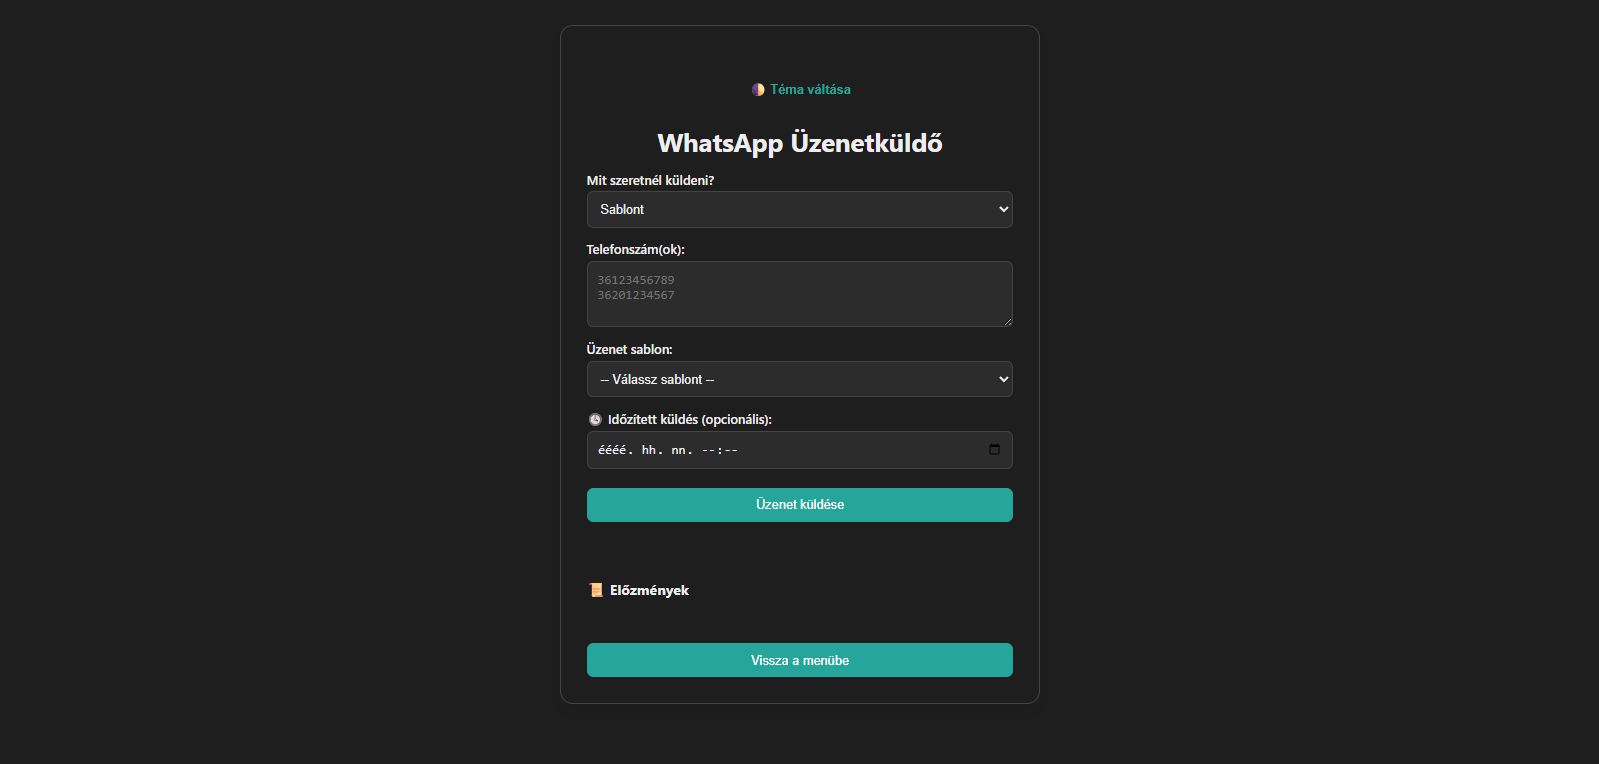
\includegraphics[width=0.95\textwidth]{images/index-html.png}
\caption{Az index.html központi üzenetküldő felülete}
\label{fig:index-html}
\end{figure}

A képernyőképen látható felület azt szemlélteti, hogy a WaccApp-ban a küldési műveletek nem különálló, egymástól elszakított funkcióként jelennek meg, hanem egy közös indítófelülethez kapcsolódnak. Ez a megoldás a felhasználó számára egyszerűbb belépési pontot ad, miközben a háttérben eltérő adatcsomagok és API-hívások indulhatnak el. A nézet ezért jól mutatja a dolgozat egyik alapvető frontendtervezési döntését: a technikai WhatsApp API-műveletek felhasználói munkafolyamattá alakítását.

A küldési folyamat frontendoldali működését jól szemlélteti az \path{index.html} egyik egyszerűsített részlete. A kódrészlet azt a részt mutatja be, ahol a felület a telefonszámokat feldolgozza, ellenőrzi, majd a kiválasztott küldési mód alapján vagy fájlküldést, vagy szöveges üzenetküldést indít.

\begin{CodeBlock}
const phonesRaw = document.getElementById('phone').value.trim();
const phones = phonesRaw
  .split(/\s|,|;/)
  .map(p => p.trim())
  .filter(p => p.length > 0);

const invalidPhones = phones.filter(p => !/^36\d{8,}$/.test(p));

if (invalidPhones.length > 0) {
  statusDiv.textContent =
    `Hibás formátumú szám(ok): ${invalidPhones.join(', ')}.`;
  statusDiv.style.color = 'crimson';
  return;
}

if (phones.length === 0) {
  statusDiv.textContent = 'Kérlek, adj meg legalább egy telefonszámot.';
  statusDiv.style.color = 'crimson';
  return;
}

statusDiv.textContent = 'Üzenet(ek) küldése...';

if (fileInput.files.length > 0) {
  phones.forEach(phone => {
    const formData = new FormData();
    formData.append('phone', phone);
    formData.append('message', fullMessage);
    formData.append('file', fileInput.files[0]);

    fetch('/send-file-message', {
      method: 'POST',
      body: formData
    })
      .then(r => r.json())
      .then(d => handleResponse(d, phone, fullMessage));
  });
} else {
  phones.forEach(phone => {
    const payload = { phone, message: fullMessage };

    fetch('/send-message', {
      method: 'POST',
      headers: { 'Content-Type': 'application/json' },
      body: JSON.stringify(payload)
    })
      .then(r => r.json())
      .then(d => handleResponse(d, phone, fullMessage));
  });
}
\end{CodeBlock}

A részlet alapján látható, hogy a frontend nem közvetlenül továbbítja a beírt adatokat, hanem először értelmezhető szerkezetbe rendezi őket. A telefonszámok többféle elválasztással is megadhatók, a kliensoldal ezekből külön címzettlistát állít elő, majd kiszűri a hibás formátumú elemeket. A validáció után a rendszer ugyanazon felületi folyamatból két eltérő küldési utat tud indítani: fájl esetén FormData alapú kérést küld a /send-file-message végpontra, egyszerű szöveges üzenet esetén pedig JSON-adatot továbbít a /send-message végpontra. Ez a megoldás jól mutatja a WaccApp frontendjének egyik lényeges szerepét: a felhasználói adatbevitelből a háttérrendszer számára feldolgozható kérést készít.

A küldési folyamatban a frontend elsődleges szerepe az, hogy a felhasználói szándékot a háttérrendszer számára feldolgozható adattá alakítsa. Ez azt jelenti, hogy a felület begyűjti a címzettet, a tartalmat, a sablonhoz tartozó paramétereket vagy a csatolt fájlt, majd a megfelelő végpont felé továbbítja a kérést. A felhasználó ebből nem az API-hívás technikai részleteit érzékeli, hanem azt, hogy a rendszer megköveteli a szükséges adatokat, jelzi a hiányzó mezőket, majd visszajelzést ad a művelet eredményéről. Ez különösen fontos, mert egy WhatsApp Business API-ra épülő rendszerben a hibás adatbevitel nemcsak lokális felületi hiba, hanem sikertelen küldési folyamat is lehet. [R13], [R14] 

A \path{messages.html} és a \path{sent-messages.html} a kommunikáció visszakövetését listaalapú formában támogatja. A beérkező és elküldött üzenetek külön nézetben történő kezelése azért hasznos, mert a felhasználó eltérő kérdésekre keres választ a két esetben. A beérkező üzeneteknél az a fontos, hogy milyen válaszok érkeztek a címzettektől, az elküldött tételeknél pedig az, hogy a rendszer milyen tartalmakat, mikor és milyen típusban továbbított. Ez a két nézet gyors ellenőrzésre alkalmas, de önmagában még nem mindig adja vissza egy teljes kommunikációs folyamat összefüggéseit. 

Ezt a hiányt a \path{conv.html} oldja fel, amely nem egyszerű adatlistaként, hanem beszélgetésfolyamként jeleníti meg a korábbi interakciókat. A nézet kontaktalapú logikája azért fontos, mert a felhasználó sokszor nem egy önálló üzenetet szeretne értelmezni, hanem azt, hogy egy adott személlyel vagy telefonszámmal milyen kommunikáció zajlott le. A bejövő és kimenő üzenetek elkülönítése, az időrendi megjelenítés és a chat-szerű forma a rendszer használatát közelebb viszi ahhoz a mintához, amelyet a felhasználók a hétköznapi üzenetküldő alkalmazásokból már ismernek. A WaccApp esetében azonban ez nem magáncélú chatélményt, hanem üzleti kommunikációs előzmények értelmezhető megjelenítését szolgálja. 

A \path{conv.html} jelentősége azért is nagy, mert a kommunikáció nem kizárólag szöveges üzenetekből áll. A beszélgetésfolyamban sablonos üzenetek, kérdőívhez kapcsolódó válaszok, képek és fájlok is megjelenhetnek. Emiatt a frontendnek nem elég egyszerű szövegsorokat listáznia, hanem többféle üzenettípust kell egységes beszélgetési kontextusba rendeznie. A beszélgetésnézet fejlesztése során az egyik gyakorlati probléma az volt, hogy a sablonos üzenetek kezdetben inkább technikai adatként jelentek meg. A felhasználó számára azonban nem az a fontos, hogy mi volt a sablon azonosítója, hanem az, hogy milyen üzenettartalom jutott el a címzetthez. Emiatt a frontendben külön figyelmet kellett fordítani arra, hogy a sablonok lehetőség szerint értelmezhető szövegként, a paraméterekkel együtt jelenjenek meg. Hasonló tanulságot adott a médiatartalmak kezelése is: egy kép fájlútvonala technikailag elegendő információ, de beszélgetési nézetben sokkal használhatóbb, ha maga a kép is megjelenik.

A beszélgetésnézet működését a \path{conv.html} képernyőképe teszi ellenőrizhetővé. Ez a nézet a korábbi kommunikáció értelmezését támogatja: a bejövő és kimenő üzenetek időrendben, chat-szerű formában jelennek meg.

\begin{figure}[H]
\centering
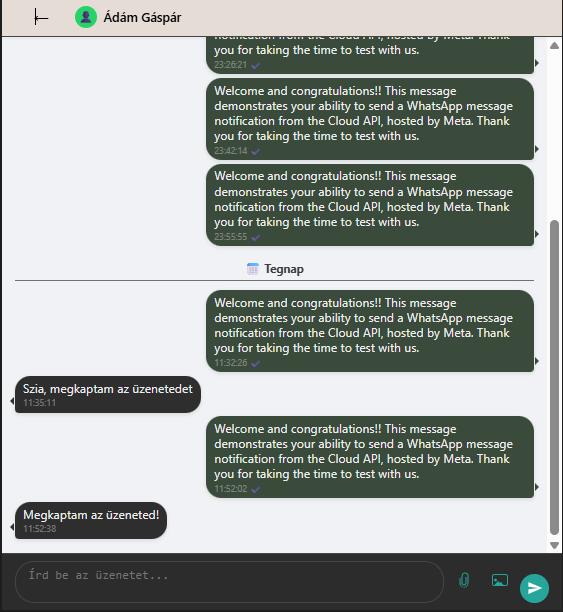
\includegraphics[width=0.95\textwidth]{images/conv-html.png}
\caption{A conv.html kontaktalapú beszélgetésnézete}
\label{fig:conv-html}
\end{figure}

A képernyőkép alapján látható, hogy a beszélgetésnézet célja a bejövő és kimenő üzenetek időrendi, olvasható visszaadása. A bejövő és kimenő üzenetek elkülönítése, az időrendi megjelenítés és a médiatartalmak értelmezhető kezelése mind azt szolgálja, hogy a felhasználó ne technikai naplót, hanem valódi beszélgetési előzményt lásson.

A beszélgetésnézetben ezt a frontendoldali értelmezést a \path{conv.html} üzenettípus szerinti feldolgozása valósítja meg. A következő egyszerűsített részlet azt mutatja, hogy a nézet külön kezeli a képeket, dokumentumokat, sablonos üzeneteket és szabad szöveges tartalmakat.

\begin{CodeBlock}
if (msg.type === 'image' || msg.type === 'media') {
  let src = normalizeMediaUrl(msg.media || msg.content || '');

  if (msg.type === 'media' && src && !isImageUrl(src)) {
    body =
    `<a href="${src}" target="_blank">Dokumentum megnyitása</a>`;
  } else {
    body = src
      ? `<img src="${src}" alt="Kép"
         style="max-width:100%; border-radius:6px;">`
      : '<em>Kép nem elérhető</em>';
  }

} else if (msg.type === 'document') {
  let link = normalizeMediaUrl(msg.media || msg.content || '');

  body = link
    ? `<a href="${link}" target="_blank">Dokumentum megnyitása</a>`
    : '<em>Dokumentum nem elérhető</em>';

} else if (msg.type === 'template') {
  const parsed = JSON.parse(msg.content || '{}');
  const tplName = parsed.template || 'ismeretlen_sablon';
  const paramValues = parsed.parameters || [];

  const templateData = templateMap[tplName];

  if (templateData && templateData.text) {
    let text = templateData.text;

    paramValues.forEach((val, i) => {
      const regex = new RegExp(`\\{\\{${i + 1}\\}\\}`, 'g');
      text = text.replace(regex, val);
    });

    body = `<div style="white-space:pre-wrap;">${text}</div>`;
  } else {
    body = '<div><em>Sablon nem található vagy üres.</em></div>';
  }

} else {
  const raw = msg.content?.trim() || '';
  body = questionMap[raw] || raw;
}
\end{CodeBlock}

A kódrészlet azért fontos, mert megmutatja, hogy a beszélgetésnézet nem nyers adatmezőket jelenít meg. A frontend először az üzenet típusát értelmezi, majd ehhez igazítja a megjelenítést. Kép esetén vizuális előnézet készül, dokumentum esetén megnyitható hivatkozás jelenik meg, sablonos üzenet esetén pedig a rendszer megpróbálja a sablon szövegét és a paramétereket emberileg olvasható üzenetté alakítani. Ez közvetlenül kapcsolódik ahhoz a fejlesztési célhoz, hogy a \path{conv.html} kommunikációs folyamatot mutasson meg.

\section{Kérdőív-szerkesztő és -küldő modul}

A WaccApp kérdőíves modulja a rendszer egyik legösszetettebb frontendrésze, mert itt a felületnek nemcsak egyszerű adatbevitelt kell biztosítania, hanem több lépésből álló kommunikációs folyamatokat kell szerkeszthetővé tennie A modul fejlesztése során két eltérő működési irány jelent meg. A \path{questionnaire.html} a szöveges vagy számalapú válaszlogikára épülő kérdőívek korábbi, rugalmasabb szerkesztési irányát képviseli, míg a \path{template.html}, a \path{template-menu.html} és a \path{template-single.html} a sablonos, gombos WhatsApp-kompatibilis kérdőívfolyamatok kezeléséhez kapcsolódik. A végleges bemutatásban a hangsúly a sablonos kérdőívlánc-szerkesztésre kerül, mert ez illeszkedik közvetlenebbül a WhatsApp Business Platform kötöttebb kommunikációs modelljéhez.

A \path{questionnaire.html} fejlesztési irányának szerepe abban állt, hogy megmutatta: a kérdőív nem kezelhető egyszerű kérdéslistaként. A szöveges vagy számalapú válaszokra épülő működésnél a kérdésekhez válaszlehetőségek és válaszfüggő következő lépések kapcsolódnak. Ez a felismerés később a sablonos kérdőívlánc-szerkesztésben is hasznosult, mert ott is ugyanaz az alapelv érvényesül: egy válasz csak akkor értelmezhető teljesen, ha ismert, hogy milyen következő kommunikációs lépést indít el.

Ebből következett, hogy a szöveges vagy számalapú kérdőíveknél a kérdéseket és válaszokat egymáshoz kapcsolódó szerkezeti elemekként kellett kezelni. Egy válasz csak akkor értelmezhető teljesen, ha ismert, hogy utána milyen következő kérdés következik, vagy a folyamat lezárul-e. Ha ez a kapcsolat hiányzik, akkor a kérdőív futás közben megszakadhat. Ezért a \path{questionnaire.html} nem csupán kitöltendő mezőket tartalmaz, hanem olyan szerkesztési helyzetet teremt, ahol a felhasználó a kérdéslánc logikáját is ellenőrizni tudja. Ez a saját frontendmegoldás azért lényeges, mert a kérdőív itt nem statikus tartalomként, hanem dinamikus kommunikációs útvonalként jelenik meg. A válaszfüggő kérdőívlogika egyszerűsített adatszerkezeti példája a 15.4. mellékletben látható, amely a kérdőíves gondolkodás alapját szemlélteti.

A sablonos kérdőívek működése ettől eltérő. A \path{template.html} a gombos, sablonalapú kérdőívfolyamatok szerkesztését támogatja, ahol a felhasználói válasz nem szabad szöveges bevitelként, hanem előre meghatározott gombos opcióként jelenik meg. A \path{template-menu.html} a sablonos feladatok közötti választást segíti, a \path{template-single.html} pedig az egyszerűbb sablonkészítési helyzetekhez kapcsolódik. Ez a különválasztás azért indokolt, mert az egyszerű sablonkészítés és a több lépésből álló sablonlánc szerkesztése nem ugyanaz a feladat. Az előbbi inkább egy adott üzenet struktúrájára koncentrál, az utóbbi viszont már egy teljes kérdőíves kommunikációs folyamatot kezel. 

A sablonos kérdőívfolyamatoknál a frontendnek alkalmazkodnia kell a WhatsApp Business Platform kötöttebb működéséhez is. A sablon neve, szövege, paraméterezése és a gombok logikája nem lehet teljesen szabad, mert a háttérben olyan platform működik, amely meghatározott formátumokat vár el. A \path{template.html} ezért olyan szerkesztési környezetet ad, amely egyszerre támogatja a felhasználói rugalmasságot és a platformlogika betartását. Ez a modul így nemcsak kényelmi szerkesztőfelület, hanem a hibás sablonláncok és megszakadó kérdőívfolyamatok megelőzésének eszköze is. [R1], [R2], [R3] 

A sablonos kérdőívfolyamatok esetében a \path{template.html} nézet mutatja meg, hogyan jelenik meg a gombos válaszokra és sablonláncokra épülő logika a frontendben. A képernyőkép azért fontos, mert a sablonos működés a WhatsApp Business Platform kötöttebb kommunikációs modelljéhez kapcsolódik.

\begin{figure}[H]
\centering
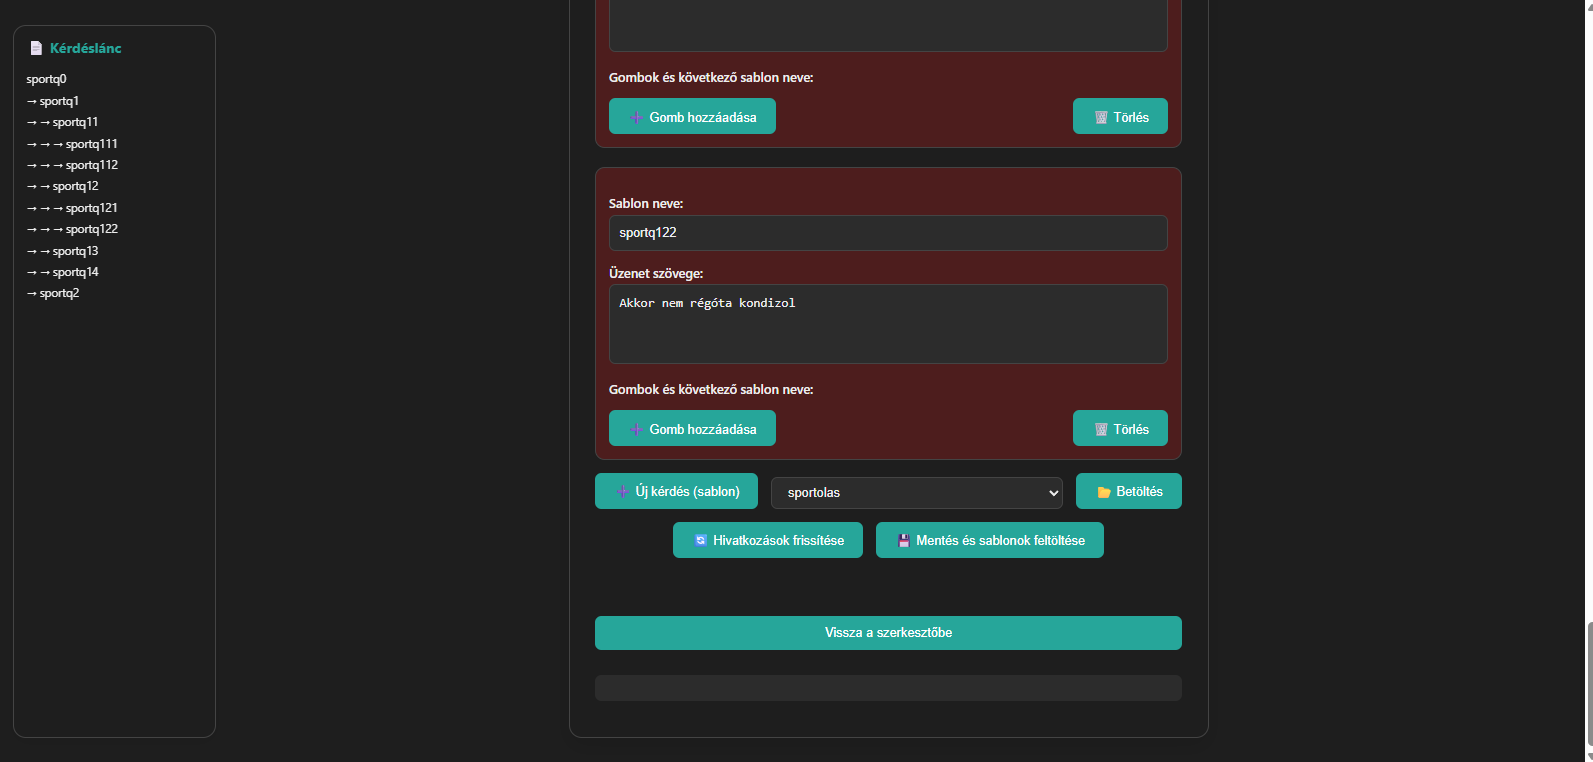
\includegraphics[width=0.95\textwidth]{images/template-html.png}
\caption{A template.html sablonos kérdőívlánc-szerkesztő felülete}
\label{fig:template-html}
\end{figure}

A \path{template.html} felületén a szerkesztés sablonokhoz, gombos válaszokhoz és következő lépésekhez kapcsolódó folyamat kialakítását jelenti. Ez a nézet jól mutatja, hogy a WaccApp frontendjében a sablonkezelés egy kommunikációs logika előkészítése. Emiatt a képernyőkép a kérdőíves modul saját fejlesztési súlyát is erősíti.

A kérdőíves modul értéke abban áll, hogy a WaccApp nemcsak elküldeni tud egy kérdést, hanem előtte lehetőséget ad a folyamat megtervezésére. A szöveges válaszlogika és a gombos sablonlogika párhuzamos kezelése azért erős saját fejlesztési elem, mert két különböző kommunikációs modellt tesz elérhetővé ugyanabban a rendszerben. A \path{questionnaire.html} rugalmasabb, szabadabb válaszokra épülő folyamatokat támogat, míg a \path{template.html} strukturáltabb, platformhoz igazított kérdőívlogikát valósít meg. A két nézet együtt adja a WaccApp kérdőíves működésének lényegét. 

\section{Szűrők és statisztikák}

A \path{filter.html} a WaccApp azon nézete, amely a korábban létrejött kommunikációs adatok visszakeresését és alapvető értelmezését támogatja. Ez a modul azért kap önálló szerepet, mert egy kommunikációs rendszerben az adatok értéke nem ér véget az üzenetek elküldésével vagy a válaszok beérkezésével. A felhasználónak később is szüksége lehet arra, hogy meghatározott címzett, időszak, üzenettípus vagy kérdőíves válasz alapján megtalálja a releváns eseményeket. A \path{filter.html} ezért nem egyszerű keresőoldal, hanem a WaccApp kommunikációs adatainak célzott értelmező felülete. 

A modul egyik legfontosabb sajátossága, hogy több szűrési feltételt képes együtt kezelni. A felhasználó név, telefonszám, üzenettípus, dátumintervallum, kérdőív, kérdés vagy válasz alapján is kereshet. Frontend szempontból ez azért összetett feladat, mert ezek a feltételek nem egymástól függetlenül hatnak. Egy dátumintervallum például szűkítheti az adott személyhez tartozó üzeneteket, az üzenettípus tovább pontosíthatja az eredményt, a kérdőívhez kapcsolódó mezők pedig a kommunikáció egy speciális részhalmazát emelhetik ki. A felületnek ezért úgy kell kezelnie a mezőket, hogy a felhasználó értelmezhető keresési helyzetet hozzon létre. 

Különösen fontos frontenddöntés volt a név és telefonszám összekapcsolása. A szűrőfelület fejlesztése közben hamar kiderült, hogy a két adat külön kezelése könnyen hibás keresési helyzetet teremthet. Ha a felhasználó egy ismert nevet választ ki, de mellette másik telefonszám marad a mezőben, akkor a rendszer technikailag ugyan lefuttathatja a keresést, az eredmény viszont félrevezető lehet. Emiatt a frontendben fontos döntés lett, hogy a név és a hozzá tartozó telefonszám egymást támogató mezőként működjön, ne pedig egymástól független szűrési adatként. Ez a részlet jól mutatja, hogy a \path{filter.html} nem csak mezőket sorol egymás alá, hanem a keresési logika helyességét is támogatja.

A név és telefonszám összekapcsolását a \path{filter.html} kliensoldali térképezéssel oldja meg. A beérkező és elküldött üzenetek feldolgozása közben a frontend név–telefonszám és telefonszám–név kapcsolatokat épít, majd ezek alapján szinkronizálja a szűrőmezőket.

\begin{CodeBlock}
contactMap = {};
nameToPhone = {};
phoneToName = {};

const incoming = inbox.map(m => {
  const phone = m.Phone_number;
  const name = m.Name || 'Ismeretlen';

  contactMap[phone] = name;
  nameToPhone[name] = phone;
  phoneToName[phone] = name;

  return {
    direction: 'received',
    name,
    phone,
    timestamp: new Date(m.Received_at),
    type: m.Type,
    content: m.Body
  };
});

nameSelect.addEventListener('change', () => {
  const name = nameSelect.value;
  const phone = nameToPhone[name] || '';
  phoneSelect.value = phone;
});

phoneSelect.addEventListener('change', () => {
  const phone = phoneSelect.value;
  const name = phoneToName[phone] || '';
  nameSelect.value = name;
});
\end{CodeBlock}

Ez a megoldás nem látványos, mégis fontos frontenddöntés. Ha a név és a telefonszám egymástól független mezőként működne, a felhasználó könnyen olyan keresést indíthatna, amelyben egy névhez hibás telefonszám társul. A szinkronizálás ezt a hibalehetőséget csökkenti, mert az egyik mező kiválasztása automatikusan igazítja a másikat. A \path{filter.html} így a keresési feltételek értelmezhetőségét is védi.

A dátumintervallum szerinti szűrés szintén lényeges része a modulnak. A felhasználó sok esetben nem egyetlen konkrét üzenetet keres, hanem egy adott időszak kommunikációs eseményeit szeretné áttekinteni. Ez különösen kérdőíves vagy kampányszerű használatnál fontos, ahol az eredmények időbeli alakulása is jelentéssel bírhat. A frontend feladata itt nemcsak két dátummező megjelenítése, hanem annak biztosítása is, hogy az intervallum értelmezhető legyen. Ha a kezdődátum későbbi, mint a záródátum, akkor a felületnek ezt hibás keresési helyzetként kell kezelnie, mert az ilyen lekérdezés félrevezető eredményt adhatna. 

Az eredmények megjelenítése a modul másik fontos része. A \path{filter.html} felületén a találatoknak olyan formában kell megjelenniük, hogy a felhasználó ne csak azt lássa, hogy léteznek adatok, hanem gyorsan értelmezni is tudja őket. A strukturált megjelenítés ebben a helyzetben azért indokolt, mert több metaadatot kell egyszerre figyelembe venni: a címzettet, az időpontot, az üzenettípust, a kérdőívet, a kérdést vagy a választ.

A \path{filter.html} képernyőképe a WaccApp visszakeresési és egyszerű válaszösszesítési működését mutatja be. A rendszer ezen része itt nem új kommunikációt indít, hanem a korábban keletkezett üzenetek és kérdőíves válaszok értelmezését támogatja.

\begin{figure}[H]
\centering
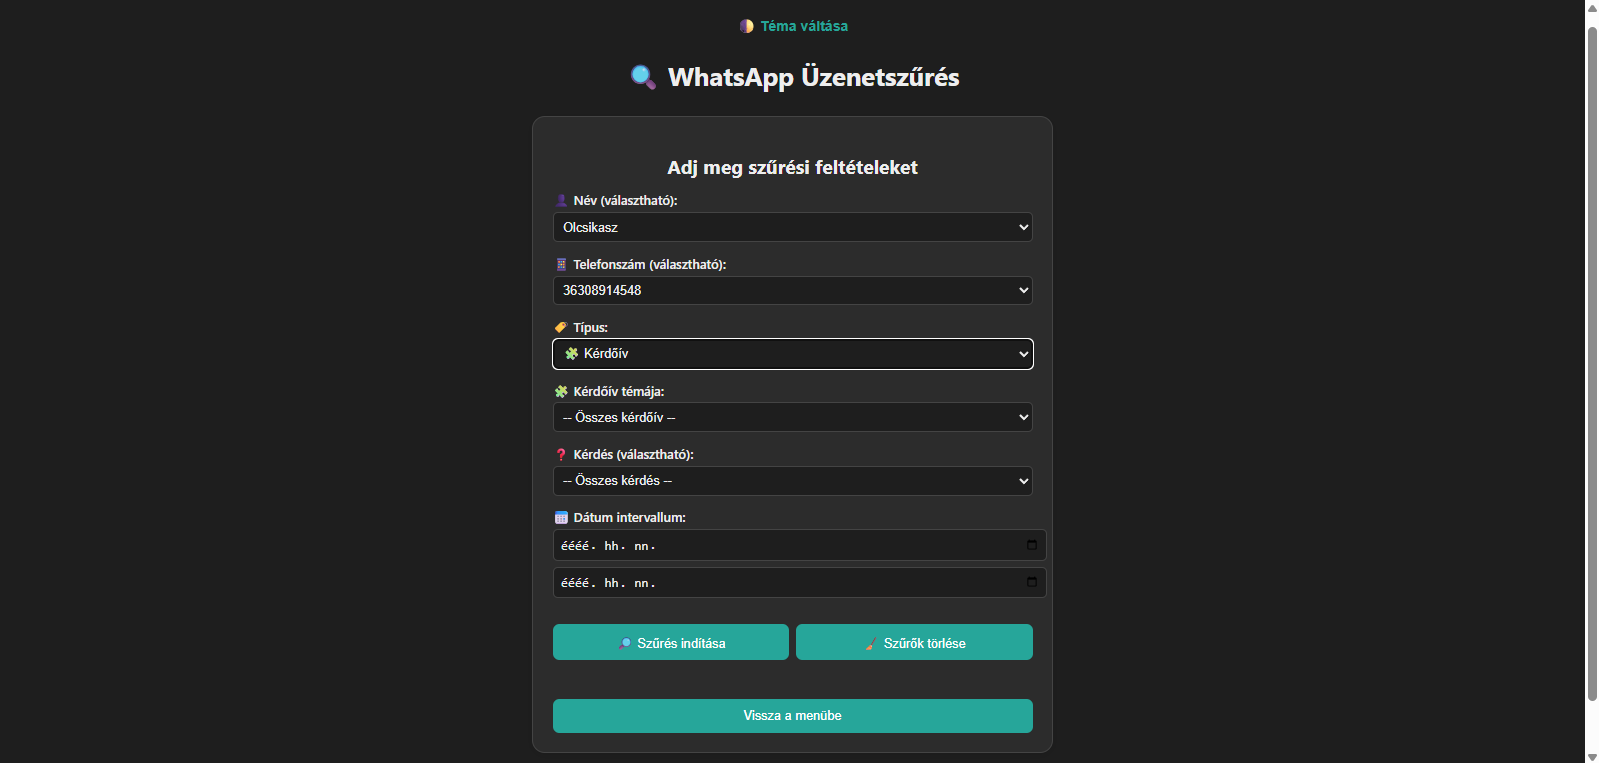
\includegraphics[width=0.95\textwidth]{images/filter-html.png}
\caption{A filter.html kérdőíves szűrési feltételeket kezelő nézete}
\label{fig:filter-html}
\end{figure}

A képernyőkép alapján látható, hogy a szűrőfelület többféle keresési szempontot kezel, például nevet, telefonszámot, dátumot, üzenettípust, kérdőívet vagy kérdést. A nézet célja, hogy a felhasználó a korábban létrejött kommunikációs és kérdőíves adatok között célzottan tudjon keresni. Az egyszerű válaszösszesítés ehhez a szűrési logikához kapcsolódik, vagyis a kérdőíves adatok értelmezését segítő kiegészítőként jelenik meg.

A modulban megjelenő alapvető statisztikai funkció nem teljes analitikai rendszert jelent, hanem kérdőíves válaszok egyszerű darabszám szerinti összesítését. Ennek működését a következő egyszerűsített kódrészlet szemlélteti.

\begin{CodeBlock}
function collectAnswerStats(theme, qid) {
  const flow = window.__flowCache?.[theme] || {};
  const node = flow[qid] || {};
  const options = Object.keys(node.next || {});

  const respondents = {};
  const otherKey = '__OTHER__';

  function addAnswer(key, phone) {
    if (!respondents[key]) respondents[key] = new Set();
    respondents[key].add(phone);
  }

  allMessages.forEach((msg, index) => {
    if (isQuestionMessage(msg, theme, qid)) {
      const reply = findFirstReplyAfter(index, allMessages);
      if (!reply) return;

      const answer = normAnswer(reply.content || '');
      const known = options.find(opt => normAnswer(opt) === answer);
      addAnswer(known || otherKey, reply.phone);
    }
  });

  const counts = {};
  options.forEach(opt => {
    counts[opt] = respondents[opt]?.size || 0;
  });

  if (respondents[otherKey]?.size) {
    counts[otherKey] = respondents[otherKey].size;
  }

  return { counts, respondents };
}
\end{CodeBlock}

A válaszösszesítés lényege, hogy a frontend a kérdőív adott kérdéséhez megkeresi a hozzá tartozó első választ, majd az ismert válaszlehetőségekhez vagy az „Egyéb” kategóriához sorolja. A Set használata azért hasznos, mert egy válaszopcióhoz címzettenként számolja a válaszadókat, nem egyszerűen nyers üzenetszámot jelenít meg.

Amikor a felhasználó kérdőíves szűrést alkalmaz, és kiválaszt egy konkrét kérdést, a felület képes megmutatni, hogy az adott válaszlehetőségekre hány válasz érkezett. A válaszok között megjelenhet az összes válasz darabszáma, az egyes ismert válaszopciókhoz tartozó darabszám, valamint egy „Egyéb” kategória is azokhoz az értékekhez, amelyek nem illeszkednek az előre ismert válaszlehetőségekhez.

Ez a megoldás elsősorban kérdőíves válaszok gyors áttekintésére alkalmas. A célja az, hogy a felhasználó rögtön lássa, mely válaszok fordultak elő, és azokhoz körülbelül mekkora válaszadói kör tartozik. A felület a kiválasztott válaszhoz kapcsolódó személyeket vagy telefonszámokat is meg tudja jeleníteni, így az összesítés nem szakad el a konkrét kommunikációs adatoktól. Ez különösen hasznos akkor, ha a felhasználó nemcsak az arányokra kíváncsi, hanem arra is, hogy egy adott válasz mely címzettekhez kapcsolódott.

Fontos korlát ugyanakkor, hogy a WaccApp jelenlegi formájában nem tartalmaz diagramokat, idősoros kimutatásokat, exportálható riportokat vagy részletes kampányelemzést. Az üzenettípus, dátumintervallum, név, telefonszám, kérdőív és válasz szerinti szűrés támogatja az adatok célzott visszakeresését, de ezek nem alkotnak teljes értékű statisztikai dashboardot. A modul ezért inkább egyszerű frontendoldali értelmező és visszakereső felületként értékelhető, amely a későbbi fejlettebb statisztikai funkciók alapját adhatja.

A szűrési és válaszösszesítési modul tehát összeköti a WaccApp operatív és értelmező oldalát. Az \path{index.html} és a kérdőíves oldalak létrehozzák vagy elindítják a kommunikációs eseményeket, a \path{messages.html}, a \path{sent-messages.html} és a \path{conv.html} visszakövethetővé teszik azokat, a \path{filter.html} pedig célzott kereséssel és egyszerű válaszösszesítéssel segíti az utólagos feldolgozást. Ez a modul azért fontos, mert általa a WaccApp nemcsak küldőfelületként működik, hanem a kommunikációs és kérdőíves adatok későbbi alapvető értelmezését is támogatja.


\section{Média- és fájlkezelés}

A média- és fájlkezelés a WaccApp kommunikációs működésének kiterjesztése. A rendszer nem kizárólag szöveges tartalmak továbbítására készült, hanem képek és dokumentumok kezelésére is alkalmas. Ez a funkció elsősorban az \path{index.html} küldőfelülethez, a \path{conv.html} beszélgetésnézethez, valamint a public/uploads és a public/sent\_media mappákhoz kapcsolódik. A modul jelentősége abban áll, hogy a fájlok nem különálló technikai mellékletekként jelennek meg, hanem a kommunikációs folyamat részeként. 

Az \path{index.html} oldalhoz kapcsolódó fájlkezelés a kiválasztással indul. A felhasználó megadja a címzettet, kiválasztja a továbbítandó fájlt, majd a rendszer a küldési folyamat részeként kezeli azt. Frontend szempontból itt az egyik legfontosabb döntés az, hogy a fájlkiválasztás ne vak művelet legyen. A felhasználónak még a küldés előtt érzékelnie kell, hogy milyen állományt választott ki, és az alkalmas-e a továbbításra. Képek esetében ezt vizuális előnézet segítheti, dokumentumok esetében pedig a fájlnév és a típus megjelenítése adhat ellenőrzési lehetőséget. 

A public/uploads és a public/sent\_media mappák eltérő szerepet töltenek be a rendszer működésében. Az uploads a feltöltött vagy előkészített állományokhoz kapcsolódik, míg a sent\_media az elküldött médiaelemek visszakövetésében kap szerepet. Ez a különbség frontend szempontból azért fontos, mert a fájlkezelés nem zárul le a kiválasztás és elküldés pillanatában. A felhasználó számára az is lényeges, hogy később a beszélgetésben vagy az előzmények között értelmezhetően vissza tudja nézni, milyen médiatartalom került továbbításra. 

A \path{conv.html} oldal különösen fontos szerepet kap a médiafájlok megjelenítésében. Ha egy elküldött kép csak hivatkozásként jelenne meg, a felhasználónak külön meg kellene nyitnia, hogy megértse, milyen tartalomról van szó. A vizuális megjelenítés ezzel szemben azonnal értelmezhetővé teszi a médiát a beszélgetés kontextusában. Ez nem apró esztétikai részlet, hanem konkrét használhatósági különbség. Egy beszélgetés visszakövetésekor a felhasználó nem fájlelérési útvonalakat akar olvasni, hanem azt szeretné látni, milyen tartalom ment ki vagy érkezett be az adott kommunikációs folyamatban. 

A média- és fájlkezelésnél a hibamegelőzés is konkrét formában jelenik meg. A nem támogatott fájltípus, a hibás kiválasztás vagy a hiányzó állomány olyan helyzet, amelyet célszerű már a küldési folyamat elején kezelni. A frontend feladata itt az, hogy a felhasználó ne csak a szerveroldali elutasítás után találkozzon a problémával, hanem már a kiválasztás vagy küldés előkészítése során visszajelzést kapjon. Ez csökkenti a félreküldés, a sikertelen feltöltés és a bizonytalan felhasználói helyzetek esélyét. [R13], [R14] 

A modul korlátja, hogy a fájlkezelés frontendoldalon csak részben ellenőrizhető. A tényleges továbbítás, tárolás és WhatsApp-platformszintű feldolgozás a háttérrendszerhez és a külső szolgáltatáshoz kapcsolódik. A frontend mégis jelentős szerepet vállal abban, hogy a felhasználó a küldés előtt és után is értelmezhető információt kapjon. A médiafunkció ezért nem egyszerű csatolmánykezelésként, hanem a kommunikáció vizuális gazdagításaként jelenik meg a WaccApp-ban. 

\section{Időzített kampányok és ütemezett küldések}

Az időzített küldések modulja az \path{index.html} küldési folyamatának kiterjesztéseként értelmezhető. A rendszer ezen a ponton nem új, teljesen különálló kommunikációs felületet hoz létre, hanem az azonnali küldés logikáját egészíti ki azzal a lehetőséggel, hogy a felhasználó egy későbbi időponthoz kösse a művelet végrehajtását. Ez a funkció szöveges üzenet, sablon, kérdőív vagy médiafájl esetében is értelmezhető, de frontend szempontból minden esetben ugyanaz a központi kérdés: a felhasználó ne csak tartalmat adjon meg, hanem a végrehajtás időpontját is egyértelműen meghatározza. 

Az időzítés felületi szempontból azért összetett, mert az időpont önmagában nem elegendő adat. Egy időzített szöveges üzenethez szükséges a címzett és az üzenettartalom, egy időzített sablonküldéshez a sablon és a paraméterek, egy kérdőívindításhoz a kiválasztott kérdőív, médiafájl esetén pedig a továbbítandó állomány. A frontendnek ezért az időzítést nem önálló mezőként, hanem a választott küldési típushoz kapcsolódó kiegészítő adatként kell kezelnie. Ez a megoldás biztosítja, hogy az időzítés ne váljon elszakított beállítássá, hanem a konkrét kommunikációs művelet részeként működjön. 

A modul egyik legfontosabb frontendfeladata az időpont értelmezhetőségének ellenőrzése. Ha a felhasználó nem ad meg időpontot, múltbeli időpontot választ, vagy olyan adatot rögzít, amely nem kapcsolható értelmesen a kiválasztott küldési módhoz, akkor a rendszernek ezt még a mentés előtt jeleznie kell. Ez különösen fontos, mert időzített műveleteknél a hiba sokszor nem azonnal derülne ki. Egy rosszul beállított időpont vagy hiányos tartalom később okozna sikertelen küldést, amikor a felhasználó már nem feltétlenül figyeli aktívan a folyamatot. 

Az időzített küldések sajátossága, hogy a művelet indítása és tényleges végrehajtása időben elválik egymástól. Az azonnali üzenetküldésnél a felhasználó rövid időn belül visszajelzést vár a küldés sikeréről vagy hibájáról. Időzítésnél viszont először a rögzítés sikeressége, később pedig a tényleges végrehajtás állapota válik fontossá. Emiatt a frontendnek nemcsak a mentés pillanatában kell visszajelzést adnia, hanem a későbbi státuszok értelmezhetőségét is támogatnia kell. A várakozó, elküldött vagy sikertelen állapotok a felhasználó számára azt mutatják meg, hogy a korábban beállított kommunikációs művelet hol tart az életciklusában. 

A modul elnevezésében szereplő kampánylogika ezért nem teljes értékű marketingautomatizálási rendszert jelent, hanem a WaccApp kommunikációs folyamatainak időbeli tervezhetőségét. Ez fontos különbség, mert a frontend jelenlegi szerepe nem egy komplex kampánymenedzsment-dashboard kiváltása, hanem az, hogy az azonnali küldések mellett előre ütemezhető műveleteket is kezelhetővé tegyen. A megoldás gyakorlati értéke abban áll, hogy a felhasználó nemcsak reagálni tud egy kommunikációs helyzetre, hanem előre is beállíthat bizonyos küldési folyamatokat. 

Az időzített küldések modulja tehát a WaccApp frontendjében a kommunikációs kontroll kiterjesztéseként jelenik meg. Az \path{index.html} továbbra is a központi indítófelület marad, de a küldés ideje már nem feltétlenül azonos a művelet rögzítésének idejével. Ez a különbség indokolja az időpontmező, a hozzá kapcsolódó validáció, valamint a későbbi státuszkövetés szerepét. 

\section{A modulok együttműködése a WaccApp frontendjében}

A WaccApp kiemelt moduljai nem önálló, egymástól független funkciók, hanem egy közös kommunikációs folyamat különböző szakaszait támogatják. A \path{login.html} és a \path{menu.html} a rendszer használatának keretét adják: előbbi a belépési pontot, utóbbi a főbb nézetek közötti eligazodást biztosítja. Az \path{index.html} elindítja az üzenetküldést, a kérdőívindítást, a médiaküldést vagy az időzített műveletet. A \path{messages.html} és a \path{sent-messages.html} listaalapú áttekintést ad a kommunikációs eseményekről. A \path{conv.html} egy adott kontakt beszélgetését rendezi értelmezhető folyamatba. A \path{questionnaire.html} és a sablonkezelő oldalak a kérdőíves kommunikáció előkészítését szolgálják, a \path{filter.html} pedig az utólagos visszakeresést és alapvető elemzést támogatja. 

Ez az együttműködés teszi a WaccApp frontendjét többé egyszerű oldalak gyűjteményénél. A rendszerben egy művelet gyakran több nézeten keresztül válik teljessé. Egy kérdőív például először a szerkesztőfelületen jön létre, később az \path{index.html} oldalról indítható, a válaszok a kommunikációs előzményekben jelennek meg, végül a \path{filter.html} segítségével visszakereshetők. Hasonló logika figyelhető meg a médiaküldésnél is: a fájl kiválasztása és küldése az indítófelülethez kapcsolódik, de az elküldött tartalom valódi értelme a beszélgetésnézetben válik láthatóvá. 

A fejezet szerepe ezért az, hogy megmutassa a WaccApp saját frontendmegoldásait működés közben. A korábbi fejezetekben szereplő követelmények, UX-döntések és architekturális alapok itt konkrét modulokká állnak össze. Az üzenetküldés, a kérdőívkezelés, a szűrés, a médiafájl-kezelés és az időzítés külön-külön is értelmezhető funkciók, de a rendszer gyakorlati értékét az adja, hogy ezek egymáshoz kapcsolódva támogatják a WhatsApp-alapú kommunikáció teljesebb kezelését. Ez a moduláris együttműködés alapot biztosít a következő fejezethez, amely már azt mutatja be, hogy a frontend nézetei milyen API-kapcsolatokon keresztül működnek együtt a háttérrendszerrel. [R1], [R10], [R13], [R14] 

\chapter{API-integráció és kliensoldali biztonság}

A WaccApp frontendjének működésében az API-integráció nem önálló technikai háttérrészlet, hanem a felhasználói műveletek közvetlen folytatása. A korábbi fejezetek bemutatták, hogy a rendszer több, feladat szerint elkülönített nézetből áll, és ezek a nézetek különböző kommunikációs, kérdőíves, szűrési, média- és időzítési folyamatokat támogatnak. Ebben a fejezetben az kerül bemutatásra, hogy a WaccApp egyes frontendműveletei milyen szerveroldali végpontokhoz kapcsolódnak, és a kliensoldal hogyan kezeli az ezekből érkező válaszokat. 

A frontend szempontjából az API-kapcsolat minden esetben egy felhasználói döntésből indul. A felhasználó üzenetet küld, sablont választ, kérdőívet indít, fájlt csatol, szűrést futtat, beszélgetést nyit meg vagy időzített műveletet állít be. A kliensoldal ezekből az adatokból állítja össze azt a kérést, amelyet a háttérrendszer felé továbbít. A válasz megérkezése után a frontend feladata az, hogy a technikai eredményt felhasználói szempontból értelmezhető állapottá alakítsa. Ez lehet sikeres küldés, hiányzó adat miatti hiba, üres találati lista, sikertelen fájlküldés, nem létező kérdőív, vagy egy időzített művelet mentésének eredménye. 

A fejezet másik fontos célja a kliensoldali felelősség határainak tisztázása. Ez különösen fontos azért, mert a WaccApp nemcsak technikai kéréseket továbbít, hanem telefonszámokkal, üzenetekkel, kérdőíves válaszokkal és médiatartalmakkal dolgozó kommunikációs felületként működik. A WaccApp frontendje nem helyettesíti a backendoldali ellenőrzést, a jogosultságkezelést vagy a WhatsApp Business Platform szabályainak érvényesítését. Ugyanakkor első védelmi és értelmezési rétegként működik: csökkenti a hibás kérések számát, segíti a helyes adatbevitelt, óvatosan kezeli a megjelenített adatokat, és a felhasználó számára láthatóvá teszi azokat a korlátozásokat, amelyek a platform- vagy adatvédelmi működésből következnek. [R10], [R11], [R12]

Az API-integráció megértéséhez érdemes a WaccApp működését rendszerarchitektúra szintjén is áttekinteni. A \ref{fig:rendszer-architektura}. ábra azt mutatja meg, hogy a felhasználói művelet hogyan halad végig a frontendrétegen, a REST API-kapcsolaton, a backend feldolgozáson, a WhatsApp Business API-integráción és az adatbázison.

\begin{figure}[H]
\centering
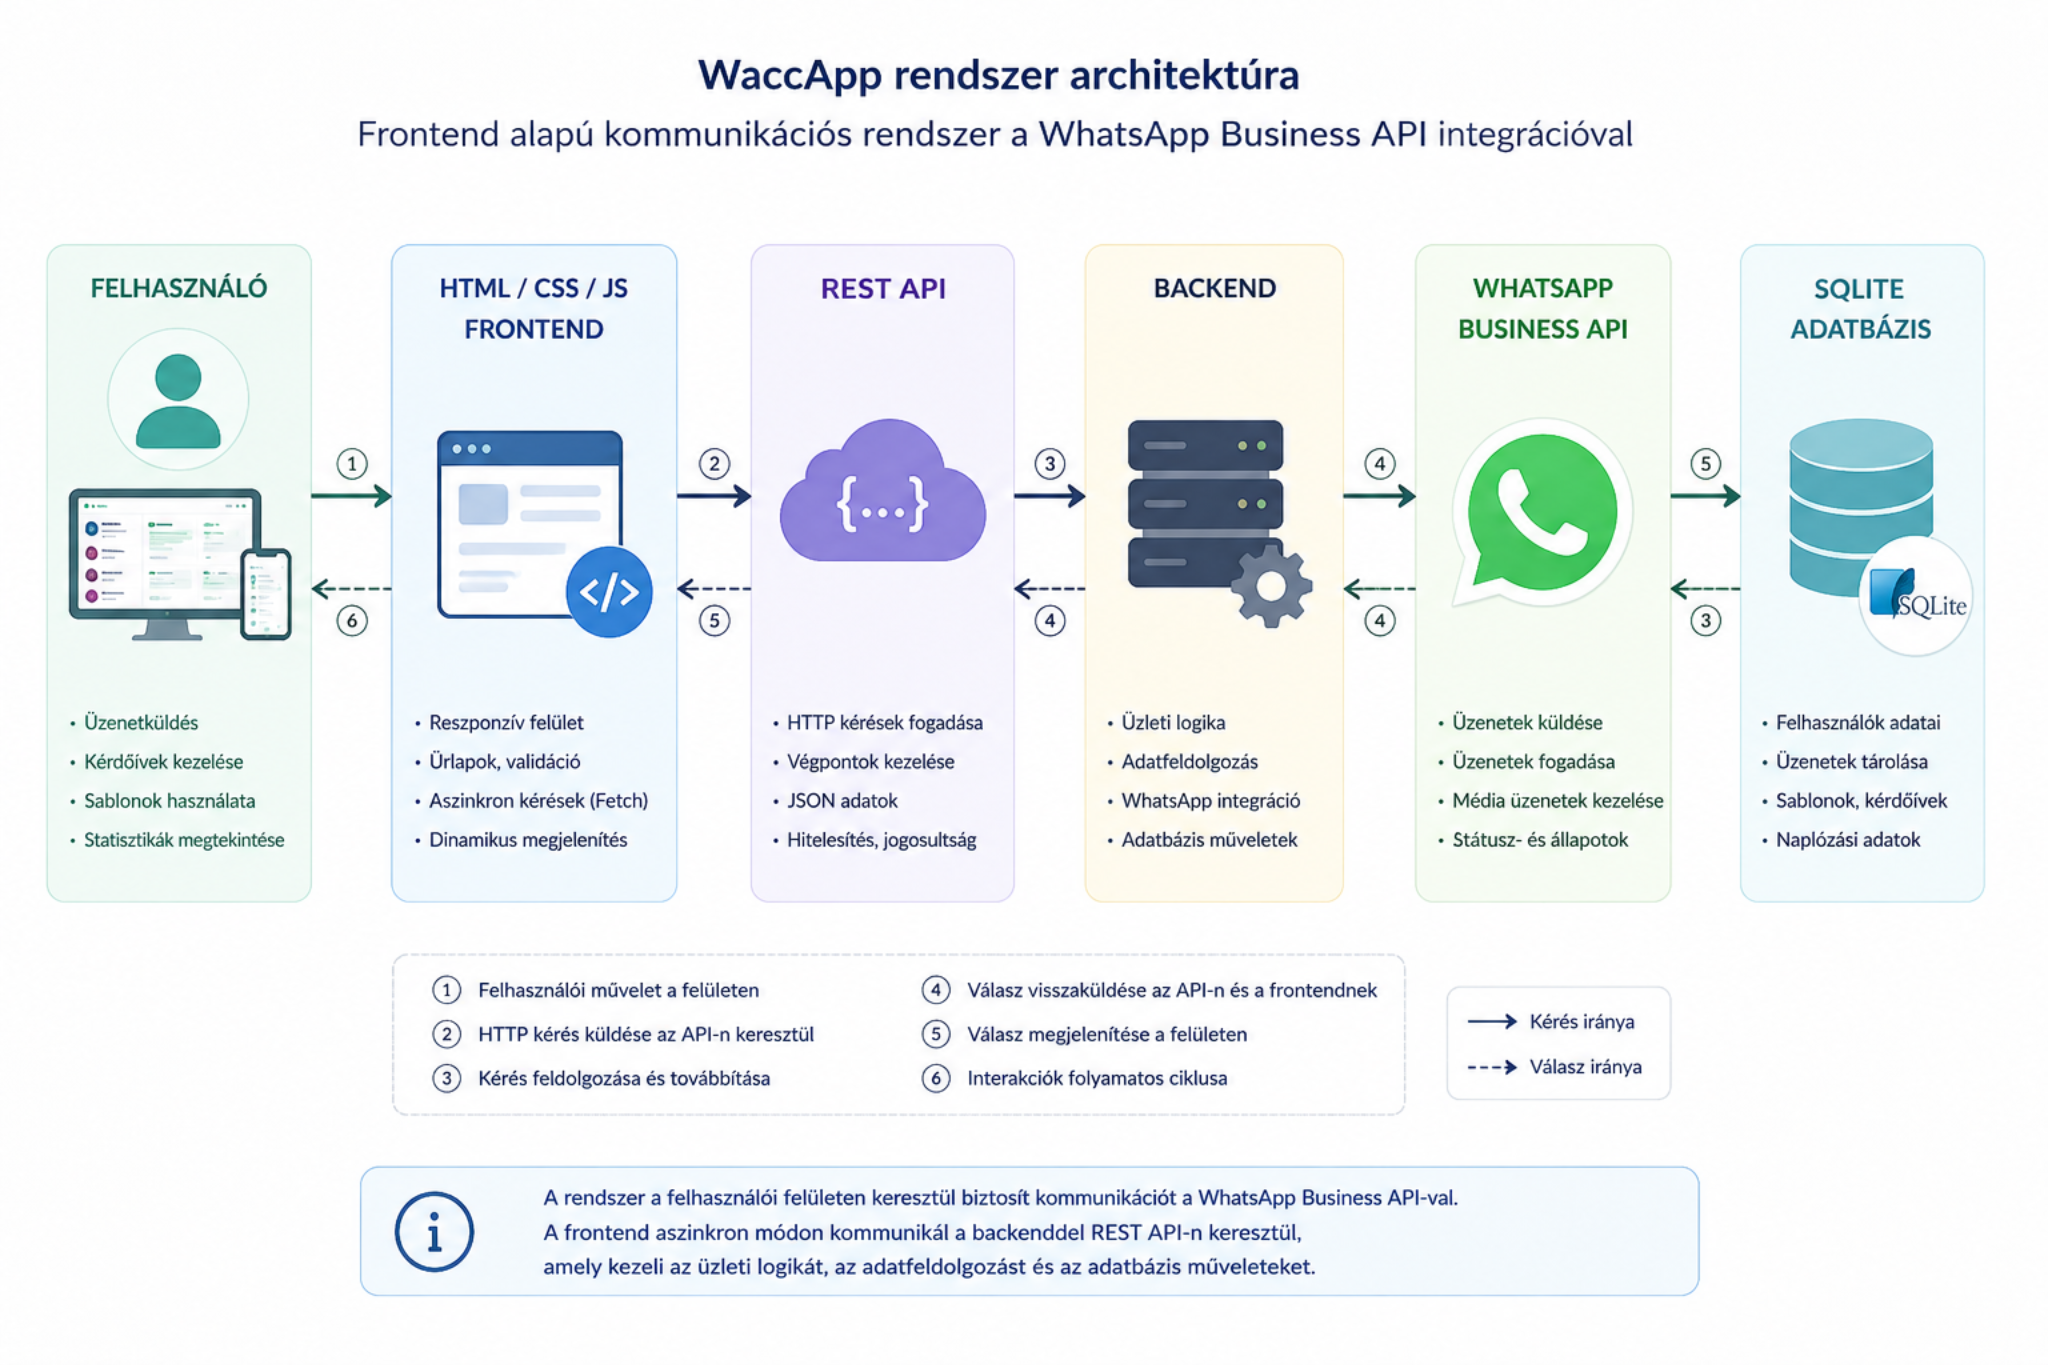
\includegraphics[width=0.95\textwidth]{images/waccapp-rendszer-architektura.png}
\caption{A WaccApp rendszer architektúrája frontend nézőpontból.}
\label{fig:rendszer-architektura}
\end{figure}

A frontend a felhasználói műveletek kiindulópontja és a visszajelzések megjelenítési helye, de a tényleges üzenetküldés, adattárolás és WhatsApp-platformmal való kommunikáció a háttérrendszeren keresztül történik. Ezért a WaccApp kliensoldala köztes értelmező rétegként működik: a felhasználó számára kezelhető űrlapokat, nézeteket és állapotokat ad, miközben a háttérben REST API-kérések kapcsolják össze a felületet a szerveroldali logikával és a külső kommunikációs platformmal.

\section{Az API-kapcsolatok szerepe a frontend moduljaiban}

A WaccApp frontendnézetei eltérő típusú API-kapcsolatokat használnak. Az \path{index.html} elsősorban műveletindító oldal, ezért innen főként olyan kérések indulnak, amelyek valamilyen kommunikációs műveletet hajtanak végre. Ide tartozik az egyedi szöveges üzenet küldése, a sablonos üzenet továbbítása, a fájl- vagy médiaküldés, a kérdőív indítása, valamint az időzített küldések rögzítése. Ebben a nézetben a frontend szerepe az, hogy a felhasználó által kiválasztott küldési módhoz igazítsa az adatokat, majd a megfelelő végpont felé továbbítsa a kérést. 

A kommunikációs előzményekhez kapcsolódó nézetek más jellegű API-kapcsolatokat igényelnek. A \path{messages.html}, a \path{sent-messages.html} és a \path{conv.html} nem elsősorban új műveleteket hoznak létre, hanem meglévő kommunikációs adatokat kérnek le és jelenítenek meg. A frontend itt a szerveroldalról érkező üzenetadatokat alakítja át listává, beszélgetésfolyammá vagy kontaktalapú nézetté. A \path{conv.html} esetében különösen fontos, hogy a beérkező adatok időrendi és típus szerinti értelmezést kapjanak, mert a felhasználó nem technikai rekordokat, hanem beszélgetést szeretne látni. 

A kérdőív- és sablonkezelő oldalak szintén saját API-kapcsolati logikával rendelkeznek. A \path{questionnaire.html} és a \path{template.html} esetében a frontend nemcsak adatokat kér le, hanem szerkesztett struktúrákat is ment. A kérdések, válaszok, elágazások, sablonnevek és gombos kapcsolatok olyan szerkezetet alkotnak, amelyet a háttérrendszernek később kérdőívindításkor vagy sablonos kommunikáció során újra fel kell tudnia használni. Emiatt ezeknél a nézeteknél az API-integráció nem egyszerű adatlekérdezés, hanem a szerkesztett kommunikációs logika tárolásának és visszatöltésének eszköze. 

A \path{filter.html} API-kapcsolatai visszakeresési és értelmezési célt szolgálnak. Ez az oldal a korábbi kommunikációs események, kérdőívválaszok és metaadatok alapján állít elő szűrt eredményeket. A frontend itt a felhasználó által megadott feltételeket, például nevet, telefonszámot, dátumintervallumot, üzenettípust vagy kérdőívhez kapcsolódó adatot alakít lekérdezhető formává. Az API-válasz alapján a felület nem pusztán adatokat ír ki, hanem áttekinthető eredménymegjelenítést biztosít. 

A belépési, adminisztratív és fiókkezelő oldalak más jellegű kapcsolatot képviselnek. A \path{login.html}, az \path{account.html} és az \path{admin.html} esetében a frontend olyan végpontokhoz kapcsolódik, amelyek a hozzáféréshez, fiókadatokhoz, adminisztratív beállításokhoz vagy hozzájárulások kezeléséhez tartoznak. Ezek a nézetek nem a kommunikációs folyamat közvetlen magját adják, de fontosak abból a szempontból, hogy a rendszer használata ellenőrzött keretek között történjen. 

\section{A frontend szempontból fontos végpontok működési csoportjai}

A WaccApp-ban az üzenetküldési folyamatokhoz több, egymástól eltérő célú végpont kapcsolódik. Az egyedi szöveges üzenetek küldését a /send-message végpont szolgálja, amelyhez a frontend jellemzően a címzettet és az üzenettartalmat továbbítja. A sablonos üzenetek esetében a /send-template végpont kap szerepet, ahol a kliensoldalnak már nemcsak címzettet, hanem sablonnevet, nyelvi beállítást és adott esetben paramétereket is kezelnie kell. A fájl- és médiaküldéshez a /send-file-message kapcsolódik, amelynél a frontendnek a szöveges adatok mellett a kiválasztott állományt is továbbítania kell. Ezek a végpontok ugyan mind küldési művelethez tartoznak, de eltérő adatbeviteli helyzetet eredményeznek, ezért az \path{index.html} felületén a mezők és ellenőrzések a választott küldési típushoz igazodnak. 

A kérdőíves és sablonos működéshez lekérdező és mentő végpontok is kapcsolódnak. Az /available-templates, az /available-template-questionnaires és a /firsttemplates a választható sablonok, sablonos kérdőívek és kezdősablonok betöltését támogatják. A /get-questionnaire/:theme és az /all-questionnaires a kérdőívek betöltéséhez és áttekintéséhez kapcsolódik. A szerkesztési oldalon a /save-to-questionnaire a kérdőíves logika mentésében kap szerepet, míg a /create-template a sablonkészítéshez kötődik. A frontend számára ezek a végpontok azért különösen fontosak, mert a kérdőívszerkesztés nem statikus űrlapkitöltés, hanem a háttérrendszerből érkező és oda visszamentett folyamatstruktúrákra épül. 

A kommunikációs előzmények és visszakereshető adatok megjelenítését elsősorban a /messages, a /sent-messages, a /contacts, a /message-metadata és a /questionnaire-themes végpontok támogatják. A /messages a beérkező vagy tárolt kommunikációs események lekéréséhez kapcsolódik, míg a /sent-messages az elküldött tételek megjelenítését segíti. A /contacts a kontaktalapú működésben fontos, mert a beszélgetésnézet és a szűrés is támaszkodhat a név és telefonszám közötti kapcsolatra. A /message-metadata és a /questionnaire-themes olyan kiegészítő adatokat biztosítanak, amelyek a szűrési és értelmezési folyamatokat támogatják. Ezek a végpontok elsősorban a \path{messages.html}, a \path{sent-messages.html}, a \path{conv.html} és a \path{filter.html} működéséhez kapcsolódnak. 

Az időzített műveletekhez a /schedule és a /schedule-media végpontok tartoznak. A /schedule az időzített szöveges, sablonos vagy kérdőíves műveletek rögzítéséhez használható, míg a /schedule-media a médiatartalomhoz kapcsolódó ütemezést támogatja. Frontendoldalon ezek a végpontok azért igényelnek külön figyelmet, mert az időzítésnél a művelet rögzítése és tényleges végrehajtása időben elválik egymástól. Az \path{index.html} ezért nemcsak azt kezeli, hogy mit szeretne küldeni a felhasználó, hanem azt is, hogy mikor történjen meg a küldés. 

Az adminisztratív és hozzáférési funkciókhoz olyan végpontok kapcsolódnak, mint az /admin/auth/login, az /admin/me, az /admin/account, az /admin/users, az /admin/consents és az ezekhez tartozó módosító vagy törlő végpontok. Ezek szerepe frontend szempontból az, hogy a belépési, fiókkezelési és adminisztratív nézetek ne közvetlenül a háttérrendszer belső működését érjék el, hanem szabályozott API-kapcsolatokon keresztül dolgozzanak. A \path{login.html}, az \path{account.html} és az \path{admin.html} így a kommunikációs moduloktól eltérő, de a rendszer egészéhez szükséges kapcsolódási réteget képviselnek.  A frontend szempontból fontosabb végpontok összefoglaló táblázata a 15.2. mellékletben található.

\section{Konkrét API-hívási példák frontend nézőpontból}

A végpontok működési csoportjai mellett érdemes néhány konkrét API-hívási példán keresztül is bemutatni, hogyan kapcsolódik a WaccApp frontendje a háttérrendszerhez. Ezek a példák azt mutatják meg, hogy a kliensoldal milyen adatot állít össze, milyen végpontra küldi azt, és a kapott válasz alapján hogyan módosítja a felület állapotát. Frontend szempontból tehát nem önmagában az API-végpont a fő kérdés, hanem az, hogy a felhasználói művelet hogyan alakul át HTTP-kéréssé, majd felhasználói visszajelzéssé.

Az egyik legegyszerűbb és legjobban értelmezhető példa az egyedi szöveges üzenet küldése. Ebben az esetben az \path{index.html} felületén a felhasználó megadja a címzett telefonszámát és az üzenet szövegét. A frontend a küldés előtt ellenőrzi, hogy a szükséges mezők ki vannak-e töltve, majd JSON-formátumban továbbítja az adatokat a /send-message végpontra.

\begin{CodeBlock}
POST /send-message
Content-Type: application/json
{
  "phone": "+36301234567",
  "message": "Szia! Ez egy teszt üzenet.",
  "content": "Szia! Ez egy teszt üzenet.",
  "theme": null
}
\end{CodeBlock}

A kérésben a phone mező jelöli a címzettet, a message mező tartalmazza a ténylegesen elküldendő szöveget, a content mező pedig a későbbi naplózás vagy kérdőíves folyamatok miatt használható kiegészítő tartalomként. Egyszerű üzenetküldésnél a message és a content értéke azonos is lehet. A theme mező opcionális, és akkor kap szerepet, ha az üzenet kérdőíves vagy tematikus kommunikációs folyamathoz kapcsolódik.

A backend válasza sikeres küldés esetén nem pusztán egy technikai státuszkód, hanem olyan JSON-válasz, amelyből a frontend eldöntheti, hogy milyen visszajelzést kell megjelenítenie a felhasználónak. Egy egyszerűsített válasz például a következő formában értelmezhető:

\begin{CodeBlock}
{
  "message": "Az üzenetküldés sikeresen lezárult",
  "results": [
    {
      "phone": "+36301234567",
      "status": "success",
      "response": {
        "messages": [
          {
            "id": "wamid.pelda_uzenetazonosito"
          }
        ]
      }
    }
  ]
}
\end{CodeBlock}

A frontend ebből elsősorban nem a WhatsApp által visszaadott belső azonosítót jeleníti meg, hanem a művelet eredményét értelmezi. Ha a results tömbben az adott címzetthez success állapot tartozik, akkor a felület sikeres küldési visszajelzést adhat. Ha ugyanebben a szerkezetben error állapot jelenik meg, akkor a frontend hibás műveletként kezeli a választ, és olyan üzenetet jelenít meg, amelyből a felhasználó érti, hogy a küldés nem zárult sikeresen.

A második példa a kommunikációs előzmények lekéréséhez kapcsolódik. A messages.html, a \path{conv.html} és részben a \path{filter.html} működéséhez szükség van a korábban beérkezett üzenetek lekérésére. Ezt a frontend a /messages végpont meghívásával éri el.

\begin{CodeBlock}
GET /messages
\end{CodeBlock}

A válasz egy üzenetrekordokat tartalmazó JSON-tömb. Egy egyszerűsített válaszrészlet például így nézhet ki:

\begin{CodeBlock}
[
  {
    "ID": 12,
    "Phone\_number": "+36301234567",
    "Name": "Teszt Elek",
    "Body": "Igen",
    "Type": "button",
    "Received\_at": "2026-05-07 10:42:15"
  },
  {
    "ID": 11,
    "Phone\_number": "+36301234567",
    "Name": "Teszt Elek",
    "Body": "Szia!",
    "Type": "text",
    "Received\_at": "2026-05-07 10:40:02"
  }
]
\end{CodeBlock}

Ebben az esetben a frontend feladata nem merül ki abban, hogy a kapott adatokat változtatás nélkül kiírja a képernyőre. A \path{messages.html} listaalapú formában jeleníti meg az üzeneteket, a \path{conv.html} pedig ugyanilyen jellegű adatokból beszélgetésfolyamot épít. A kliensoldal a Phone\_number, Name, Body, Type és Received\_at mezők alapján dönti el, hogy melyik kontakthoz tartozik az üzenet, milyen tartalom jelenjen meg, milyen típusú üzenetről van szó, és az időrendben hol kell elhelyezni azt. A felhasználó így nem adatbázisrekordokat lát, hanem értelmezhető kommunikációs előzményt.

Hasonló logikát használ az elküldött üzenetek lekérése is. A /sent-messages végpont azokat a tartalmakat adja vissza, amelyeket a rendszer korábban elküldött. Ez különösen a \path{sent-messages.html}, a \path{conv.html} és a \path{filter.html} szempontjából fontos.

\begin{CodeBlock}
GET /sent-messages
[
  {
    "id": 25,
    "phone": "+36301234567",
    "type": "text",
    "content": "Szia! Ez egy teszt üzenet.",
    "timestamp": "2026-05-07 10:39:51",
    "media\_url": null,
    "wa_message\_id": "wamid.pelda_uzenetazonosito",
    "theme": null
  }
]
\end{CodeBlock}

A beérkező és elküldött üzenetek szerkezete nem teljesen azonos, ezért a frontendnek ezeket egységes megjelenítési formára kell alakítania. A \path{conv.html} például a beérkező üzeneteket és az elküldött üzeneteket közös időrendi beszélgetésként jeleníti meg. Ehhez a kliensoldalnak irányt kell rendelnie az üzenetekhez, vagyis meg kell különböztetnie, hogy received vagy sent típusú kommunikációs eseményről van szó. Ez a frontend szempontjából fontos átalakítás, mert a felhasználó egy összefüggő beszélgetést akar látni.

A harmadik példa a \path{filter.html} működéséhez kapcsolódik. Ennél a modulnál fontos pontosítani, hogy a WaccApp jelenlegi formájában nem egyetlen külön szűrési végpontot használ minden feltétel kiszolgálására. A \path{filter.html} több meglévő végpontról tölti be az adatokat, majd a szűrési feltételek jelentős részét kliensoldalon alkalmazza. Ez a megoldás a jelenlegi rendszer méretéhez illeszkedik, mert a szűrőfelületnek elsősorban a meglévő üzenet- és kérdőíves adatok áttekinthető visszakeresését kell támogatnia.

A \path{filter.html} működéséhez például a következő lekérések kapcsolódhatnak:

\begin{CodeBlock}
GET /messages
GET /sent-messages
GET /available-templates
GET /questionnaire-themes
GET /get-questionnaire/ugyfel_elegedettseg
\end{CodeBlock}

A /questionnaire-themes végpont a kérdőíves témák listáját adja vissza, a /get-questionnaire/:theme pedig egy kiválasztott kérdőív kérdéseit és válaszlogikáját tölti be. Egy egyszerűsített kérdőívlekérési válasz például így nézhet ki:

\begin{CodeBlock}
{
  "q1": {
    "text": "Elégedett volt a szolgáltatással?",
    "next": {
      "Igen": "q2",
      "Nem": "q3"
    }
  },
  "q2": {
    "text": "Ajánlaná másoknak is?",
    "next": {
      "Igen": "end",
      "Nem": "end"
    }
  }
}
\end{CodeBlock}

A \path{filter.html} ebből a válaszból szűrőfelületet épít fel. A kérdések szövegei bekerülnek a legördülő mezőkbe, a válaszlehetőségek pedig alapot adnak az egyszerű válaszösszesítéshez. Amikor a felhasználó kiválaszt egy kérdőívet és egy konkrét kérdést, a frontend a korábban betöltött beérkező és elküldött üzenetek alapján megkeresi az adott kérdéshez kapcsolódó válaszokat, majd darabszám szerint összesíti azokat.

Egy ilyen kliensoldali szűrési állapot például a következő adatokból állhat össze:

\begin{CodeBlock}
{
  "name": "Teszt Elek",
  "phone": "+36301234567",
  "type": "questionnaire",
  "startDate": "2026-05-01",
  "endDate": "2026-05-07",
  "theme": "ugyfel_elegedettseg",
  "questionText": "q1"
}
\end{CodeBlock}

Ez az objektum nem feltétlenül önálló backendkérésként kerül továbbításra, hanem a \path{filter.html} belső állapotát szemlélteti. A frontend e feltételek alapján szűri a már lekért adatokat. A megoldás frontendoldali visszakeresést és egyszerű válaszösszesítést valósít meg, amely a jelenlegi célokhoz elegendő, de később külön szerveroldali szűrési vagy riportkészítő végponttal továbbfejleszthető.

Az API-hívási példák alapján látható, hogy a WaccApp frontendje három eltérő API-használati mintát alkalmaz. Az első a műveletindító kérés, ilyen a /send-message, ahol a felhasználói adatbevitelből küldési kérés lesz. A második az adatlekérő kérés, ilyen a /messages és a /sent-messages, ahol a frontend meglévő kommunikációs adatokat alakít át listává vagy beszélgetésnézetté. A harmadik az összetett kliensoldali értelmezés, amely a \path{filter.html} működésében jelenik meg: több végpontról érkező adatból a böngésző állít elő szűrt eredményt és egyszerű válaszösszesítést

\section{WaccApp-specifikus hibakezelési helyzetek}

A rendszer egyik leggyakoribb hibaforrása a hibás vagy hiányos adatbevitel lehet. Egy szöveges üzenetnél ilyen a hiányzó címzett vagy üres üzenettartalom. Sablonos küldésnél tipikus probléma lehet a hiányzó sablonnév, a nem megfelelő nyelvi beállítás vagy a ki nem töltött sablonparaméter. Médiafájl küldésekor a nem támogatott fájltípus, a hiányzó fájl vagy a sikertelen feltöltés okozhat hibát. Ezekben az esetekben a frontend feladata az, hogy a felhasználó lehetőleg már a kérés elküldése előtt megértse, miért nem indítható el a művelet. 

A kérdőíves moduloknál a hibák nemcsak mezőszintűek, hanem logikai jellegűek is lehetnek. A \path{questionnaire.html} esetében előfordulhat, hogy egy válaszhoz nem tartozik következő kérdés, vagy a kérdőív szerkezete nem alkot bejárható folyamatot. A \path{template.html} esetében a sablonos kérdőívlánc szakadhat meg, ha egy gombos válaszhoz nem kapcsolódik megfelelő következő sablon, vagy a sablon neve nem egyezik a háttérrendszer által kezelhető struktúrával. Ilyenkor a hiba nem egyszerűen formai probléma, hanem a későbbi kommunikációs folyamat megszakadását okozhatja. A frontend ezért ezeknél a műveleteknél nemcsak adatbeviteli, hanem folyamatértelmezési szerepet is betölt. 

A szűrési és beszélgetésnézeti hibák másképp jelennek meg. A \path{filter.html} esetében a felhasználó olyan feltételeket is megadhat, amelyek nem eredményeznek találatot, vagy logikailag félrevezető keresést hoznának létre. Ilyen lehet például a rosszul megadott dátumintervallum, a névhez nem illeszkedő telefonszám, vagy egy olyan kérdőíves feltétel, amelyhez nincs adat. Ebben a helyzetben az üres találati lista önmagában nem feltétlenül hiba, de a felületnek világossá kell tennie, hogy a lekérdezés lefutott, csak nem adott eredményt. A \path{conv.html} esetében hasonlóan fontos, hogy a beszélgetésbetöltés sikertelensége vagy az üres kommunikációs előzmény ne tűnjön rendszerhibának. 

Az időzített műveleteknél a hibakezelés különösen érzékeny, mert a művelet rögzítése és tényleges végrehajtása időben elválik egymástól. Ha a felhasználó múltbeli időpontot ad meg, nem választ ki küldendő tartalmat, hiányosan tölti ki a sablonparamétereket, vagy médiaütemezésnél nem csatol fájlt, akkor a frontendnek ezt még a mentés előtt jeleznie kell. Ellenkező esetben a hiba csak később, a tervezett küldés időpontjában válna láthatóvá, ami sokkal nehezebben értelmezhető helyzetet teremtene. 

A szerveroldali vagy platformszintű hibák esetében a frontend mozgástere kisebb, de a felhasználói visszajelzés ekkor is fontos. Előfordulhat hálózati hiba, szerveroldali feldolgozási hiba, WhatsApp Business Platform általi visszautasítás, vagy olyan eset, amikor a címzett nem alkalmas az adott típusú üzleti kommunikáció fogadására. Ilyenkor a frontend nem tudja megoldani a platformszintű problémát, de segíthet abban, hogy a felhasználó ne egy érthetetlen technikai állapottal találkozzon. A cél az, hogy a hibaüzenet legalább azt jelezze, melyik művelet nem sikerült, és a felhasználó javíthat-e valamilyen adatot, vagy a probléma a háttérrendszerhez, illetve a külső platformhoz kapcsolódik. [R13], [R14] 

\section{Kliensoldali biztonsági megfontolások}

A WaccApp frontendjének biztonsági szerepe elsődlegesen megelőző és korlátozó jellegű. A kliensoldal nem tekinthető végső biztonsági rétegnek, mert a felhasználó böngészőjében futó kód önmagában nem garantálhat teljes védelmet. A tényleges hitelesítés, jogosultságkezelés, adatbázisvédelem, szerveroldali validáció és platformszintű ellenőrzés a háttérrendszer feladata. A frontend mégis fontos szerepet tölt be, mert meghatározza, hogy a felhasználó milyen műveleteket lát, milyen adatokat adhat meg, és milyen hibás kérések indítását lehet már a kliensoldalon megakadályozni. 

Az inputellenőrzés biztonsági és megbízhatósági szűrőként értelmezhető. A telefonszámformátum ellenőrzése, a kötelező mezők vizsgálata, a sablonparaméterek meglétének ellenőrzése, a kérdőívkapcsolatok következetessége és a fájltípusok szűrése mind azt szolgálja, hogy a frontend ne engedjen tovább nyilvánvalóan hibás kéréseket. Ez csökkenti a szerver terhelését, a félreérthető hibák számát és azokat a helyzeteket, amikor a felhasználó nem tudja, miért nem működött egy művelet. 

A kliensoldali biztonság része az is, hogy a felület csak a szükséges adatokat kérje be és jelenítse meg. Egy kommunikációs rendszerben a telefonszámok, üzenetek, kérdőíves válaszok és adminisztratív adatok érzékeny információnak tekinthetők. A frontendnek ezért törekednie kell arra, hogy az adott nézetben csak olyan adatok jelenjenek meg, amelyek a felhasználói művelethez valóban szükségesek. A \path{filter.html} esetében például a találatok megjelenítésekor az áttekinthetőség mellett arra is figyelni kell, hogy a felület ne tegye indokolatlanul túl részletessé az adatmegjelenítést. A \path{conv.html} esetében a kommunikációs előzmények megjelenítése szükséges, de ennek is a beszélgetés értelmezését kell szolgálnia, nem az adatok kontroll nélküli halmozását. 

A jogosultsági és adminisztratív működésnél a frontend szerepe elsősorban a felületi hozzáférés kereteinek biztosítása. A \path{login.html}, az \path{account.html} és az \path{admin.html} nézetek olyan részei a rendszernek, amelyek a belépéshez, fiókkezeléshez és adminisztratív műveletekhez kapcsolódnak. A frontend itt nem önállóan dönti el, hogy a felhasználó mire jogosult, hanem a backend válaszaihoz igazodva jeleníti meg vagy korlátozza az elérhető műveleteket. Ez fontos szakmai határ: a kliensoldali korlátozás segíti a használhatóságot és az eligazodást, de nem helyettesítheti a szerveroldali jogosultságellenőrzést. 

A fájlkezelés szintén biztonsági szempontból érzékeny terület. A frontend előzetesen ellenőrizheti a kiválasztott fájl típusát és alapvető jellemzőit, de nem tekintheti ezt végleges védelemnek. A fájl tényleges elfogadása, tárolása és továbbítása szerveroldali kontrollt igényel. A kliensoldali ellenőrzés ennek ellenére hasznos, mert már a kiválasztás pillanatában csökkentheti a hibás műveletek számát, és érthetőbbé teheti a felhasználó számára, hogy milyen típusú tartalmak küldhetők a rendszeren keresztül. 

\section{A frontend oldaláról releváns adatvédelmi szempontok}

A WaccApp olyan kommunikációs rendszer, amely telefonszámokkal, üzenetszövegekkel, kérdőíves válaszokkal, médiafájlokkal és adminisztratív adatokkal dolgozik. Emiatt az adatvédelmi szempontok nemcsak a backend vagy az adatbázis szintjén jelennek meg, hanem a felhasználói felületen is. A frontend az a réteg, ahol a felhasználó adatot ad meg, kommunikációt indít, eredményeket keres vissza és korábbi beszélgetéseket tekint meg. Ezért a felületnek úgy kell támogatnia a munkát, hogy közben ne ösztönözzön indokolatlan adatbekérésre, felesleges adatmegjelenítésre vagy a platformszabályokkal ellentétes használatra.

A frontend szempontjából az egyik legfontosabb adatkezelési kérdés az, hogy a felhasználó pontosan milyen személyes vagy kommunikációs adatokat lát és ad meg. Egy üzenetküldésnél a címzett telefonszáma és az üzenet tartalma szükséges adat. Egy kérdőív indításánál ehhez kapcsolódhat a kiválasztott kérdőív vagy sablon neve, a válaszlehetőségek szerkezete és a későbbi válaszok visszakereshetősége. Médiafájl küldésekor maga a fájl is érzékenyebb adat lehet, mert nemcsak szöveges információt, hanem képi vagy dokumentumalapú tartalmat is hordozhat. Emiatt a frontendnek minden ilyen műveletnél egyértelműen kell jeleznie, hogy a felhasználó milyen adatot készül továbbítani.

A WhatsApp Business Platformhoz kapcsolódó üzleti kommunikáció egyik fontos feltétele az előzetes hozzájárulás, vagyis az opt-in megléte. Frontendoldalon ez nem azt jelenti, hogy a kliensoldal önállóan igazolja a hozzájárulás jogszerűségét, hanem azt, hogy a felületnek figyelembe kell vennie az ilyen korlátozásokat, és nem szabad azt sugallnia, hogy bármely telefonszám korlátlanul elérhető üzleti üzenetekkel. Ha egy címzett esetében a kommunikáció korlátozott, vagy a háttérrendszer a platformszabályok miatt visszautasít egy műveletet, akkor a frontend feladata az, hogy ezt ne nyers technikai hibaként, hanem érthető, felhasználóbarát visszajelzésként jelenítse meg. [R3], [R5]

Az adatminimalizálás frontendoldali jelentősége abban áll, hogy a felületnek csak azokat az adatokat kell bekérnie, amelyek az adott művelethez ténylegesen szükségesek. Egy szöveges üzenetküldéshez nincs szükség kérdőíves metaadatokra, egy fájlküldéshez nem kell felesleges szűrési feltételeket megadni, egy szűrési művelethez pedig csak azok a keresési szempontok relevánsak, amelyeket a felhasználó valóban használni akar. Ez a szemlélet a WaccApp többnézetes felépítésével is összhangban van, mert az egyes oldalak nem minden adatot kérnek be egyszerre, hanem az adott funkcióhoz kapcsolódó információkra koncentrálnak.

A korábbi kommunikációs adatok megjelenítésekor az átláthatóság és a visszafogottság egyensúlyára van szükség. A beszélgetésnézet, az üzenetlisták és a szűrési felület célja az, hogy a felhasználó vissza tudja követni a kommunikációt, de ez nem jelentheti azt, hogy a frontend feleslegesen túl sok adatot jelenítsen meg. A beszélgetésnézetben a kommunikációs kontextus megértése a cél, a szűrőfelületen pedig az, hogy a találatok értelmezhetők legyenek. Emiatt az adatmegjelenítésnek mindig a felhasználói feladatot kell szolgálnia: annyi információt kell láthatóvá tenni, amennyi a művelet megértéséhez szükséges, de kerülni kell az indokolatlan adatismétlést és túlzsúfolt megjelenítést.

A fájl- és médiakezelés adatvédelmi szempontból külön figyelmet igényel. A frontend ugyan nem tudja teljes körűen eldönteni, hogy egy feltöltött fájl tartalma adatvédelmi szempontból megfelelő-e, de segítheti a felelős használatot azzal, hogy a kiválasztott fájlt láthatóvá teszi a küldés előtt, ellenőrzi az alapvető fájltípust, és nem indítja el a küldést hiányos adatokkal. Ez különösen fontos, mert egy tévesen kiválasztott dokumentum vagy kép elküldése nagyobb következménnyel járhat, mint egy egyszerű űrlaphiba. A frontend szerepe ebben az esetben nem a teljes tartalmi ellenőrzés, hanem a küldés előtti tudatosítás és hibamegelőzés.

Az adatvédelmi tájékoztatás szempontjából a \path{privacy.html} külön szerepet kap a rendszerben. Ez a nézet nem kommunikációs műveletet indít, hanem a felhasználó tájékoztatását támogatja. Frontend szempontból ez azért fontos, mert az adatkezelés nemcsak háttérfolyamat, hanem olyan információ, amelynek a felhasználó számára is elérhetőnek kell lennie. A tájékoztatás, az adatminimalizálás, az opt-in szemlélet és a visszafogott adatmegjelenítés együtt biztosítják, hogy a WaccApp frontendje ne csak működőképes, hanem felelősen használható felületként jelenjen meg.

\section{A kliensoldali felelősség határai}

A WaccApp frontendjének API-integrációja azt mutatja meg, hogy a kezelőfelület nem önállóan működő technikai sziget, hanem a háttérrendszerrel együtt alkot teljes alkalmazást. Az \path{index.html} a küldési végpontokra támaszkodik, a kérdőíves oldalak a sablon- és kérdőívadatok lekérését és mentését használják, a \path{messages.html}, a \path{sent-messages.html}, a \path{conv.html} és a \path{filter.html} a kommunikációs adatok lekérésén keresztül működnek, az időzített küldések pedig külön ütemezési végpontokhoz kapcsolódnak. Ez a kapcsolatrendszer adja meg azt a technikai alapot, amelyre a felhasználó által érzékelt működés ráépül. 

A fejezet legfontosabb tanulsága, hogy a frontend felelőssége nem azonos a backend felelősségével. A kliensoldal nem döntheti el véglegesen a jogosultságokat, nem garantálhatja önmagában az adatbiztonságot, és nem helyettesítheti a szerveroldali validációt. Amit viszont megtehet, az nagyon is lényeges: segíti a helyes adatbevitelt, megakadályozza a nyilvánvalóan hibás műveletek elindítását, értelmezhetővé teszi a szerver válaszait, és a felhasználó számára láthatóvá teszi a folyamatok állapotát. 

A WaccApp esetében ez a kliensoldali felelősség különösen fontos, mert a rendszer külső kommunikációs platformra épül. Egy sikertelen üzenetküldés, hiányzó sablonparaméter, hibás kérdőívkapcsolat, nem támogatott médiafájl vagy rosszul megadott időzítés nem pusztán technikai kellemetlenség, hanem a kommunikációs folyamat megszakadását okozhatja. A frontend ezért köztes értelmező rétegként működik a felhasználó és a háttérrendszer között. Nem veszi át a backend szerepét, de segít abban, hogy a felhasználó a lehető legtöbb helyzetben időben, érthetően és javítható módon találkozzon a problémákkal. 

\chapter{Tesztelés és minőségbiztosítás}

A WaccApp frontendjének tesztelése a fejlesztési folyamat fontos visszacsatolási szakasza volt. A rendszer esetében nem volt elegendő azt ellenőrizni, hogy az egyes oldalak megnyílnak-e, vagy hogy a fő gombok technikailag elindítanak-e egy műveletet. Egy WhatsApp Business API-ra épülő kommunikációs felületnél a használhatóság ugyanúgy része a minőségnek, mint a funkcionális működés. A felhasználónak értenie kell, milyen adatot kell megadnia, mikor indítható el egy küldés, mit jelent egy hibaüzenet, és hol tudja később visszakeresni az elküldött vagy beérkezett tartalmakat.

A tesztelés ezért elsősorban a WaccApp tényleges felhasználói folyamataira épült. Az ellenőrzések középpontjában az \path{index.html} küldőfelülete, a \path{conv.html} beszélgetésnézete, a \path{messages.html} és a \path{sent-messages.html} listaoldalai, a \path{questionnaire.html} és a \path{template.html} kérdőíves felületei, valamint a \path{filter.html} szűrési nézete állt. Ezek az oldalak a korábbi fejezetekben külön modulokként jelentek meg, a tesztelés során azonban az volt a lényeges, hogy együtt is működőképes kommunikációs folyamatot alkossanak.

A minőségbiztosítás során nemcsak a sikeres eseteket kellett kipróbálni, hanem azokat a helyzeteket is, amelyek a valós használatban bizonytalanságot okozhatnak. Ilyen lehet a hibás telefonszám, az üres üzenetmező, a hiányzó sablonparaméter, a nem megfelelő fájl, a hibás kérdőívkapcsolat, a rosszul megadott dátumintervallum vagy egy olyan szűrés, amely nem ad találatot. Ezek a hibák nem mindig látványos rendszerleállásként jelennek meg. Sokszor éppen az a probléma, hogy a felület működik, de a felhasználó nem kap elég egyértelmű választ arra, hogy mi történt. A tesztelés egyik célja ezért az volt, hogy ezek a bizonytalan helyzetek felismerhetők és javíthatók legyenek.

A tesztelés közben többször előfordult, hogy egy funkció technikailag működött, használat közben mégis bizonytalannak érződött. Ilyen helyzet volt például, amikor egy művelet elindult, de a felület nem adott elég gyors visszajelzést, vagy amikor egy üres találati lista mellett nem volt egyértelmű, hogy valóban nincs adat, vagy a lekérdezés nem futott le. Ezek a tapasztalatok megerősítették, hogy a frontend tesztelésénél nemcsak a sikeres API-választ, hanem a felhasználó által érzékelt folyamatot is vizsgálni kell.

\section{A tesztelés célja és szempontrendszere}

A tesztelés elsődleges célja annak igazolása volt, hogy a WaccApp fő frontendfolyamatai a gyakorlatban is végigvihetők. Ez nemcsak azt jelentette, hogy az egyes funkciók külön-külön elérhetők, hanem azt is, hogy a felhasználó egy teljes kommunikációs munkafolyamatot el tud végezni. Egy üzenet vagy kérdőív előkészítése, elküldése, állapotának értelmezése, majd későbbi visszakeresése csak együtt ad teljes képet a rendszer működéséről.

A tesztelési szempontrendszer első része a funkcionális működés ellenőrzése volt. Az \path{index.html} oldalon azt kellett kipróbálni, hogy elindíthatók-e az egyedi szöveges üzenetek, a sablonos üzenetek, a kérdőívek, a médiafájlok és az időzített műveletek. A \path{messages.html}, a \path{sent-messages.html} és a \path{conv.html} esetében az volt a kérdés, hogy a kommunikációs adatok áttekinthetők-e, elkülönülnek-e a bejövő és kimenő tartalmak, valamint egy adott kontakt beszélgetése értelmezhető formában jelenik-e meg. A \path{questionnaire.html} és a \path{template.html} tesztelésekor a kérdések, válaszok, sablonok és következő lépések kezelése került előtérbe. A \path{filter.html} ellenőrzése pedig arra irányult, hogy a megadott feltételek alapján valóban értelmezhető eredmények jelenjenek meg.

A második szempont a hibás vagy hiányos adatbevitel kezelése volt. A WaccApp nem tekinthető megbízható frontendnek, ha csak ideális kitöltés mellett működik. Ezért külön figyelmet kaptak azok az esetek, amikor a felhasználó hibás telefonszámot ad meg, üresen hagyja az üzenetmezőt, nem tölti ki a sablonparamétereket, fájl nélkül próbál médiát küldeni, vagy időzített műveletnél hiányzó, illetve múltbeli időpontot választ. Ezeknél a teszteknél nem az volt a cél, hogy a frontend minden hibát automatikusan kijavítson, hanem az, hogy a hiba oka érthetően jelenjen meg, és a felhasználó tudja, mit kell módosítania.

A harmadik szempont a használhatóság és a reszponzív működés ellenőrzése volt. A WaccApp több különálló HTML-nézetből épül fel, ezért fontos volt megvizsgálni, hogy a felület kisebb kijelzőn is használható marad-e. Az \path{index.html} esetében a küldési mezők és gombok kezelhetősége, a \path{conv.html} esetében a beszélgetés görgethetősége és olvashatósága, a \path{filter.html} esetében pedig a több szűrési mező áttekinthetősége volt meghatározó. A kérdőívszerkesztő oldalaknál külön figyelmet igényelt, hogy a kérdések, válaszok és kapcsolódások kisebb képernyőn is követhető sorrendben jelenjenek meg.

A negyedik szempont a regressziós ellenőrzés volt. A WaccApp fejlesztése során több funkció egymásra épült, ezért egy módosítás könnyen hatással lehetett más nézetekre is. Egy kérdőíves logikai javítás például érinthette az \path{index.html} kérdőívindítását, a \path{conv.html} beszélgetésmegjelenítését vagy a \path{filter.html} kérdőíves szűrését. Emiatt egy-egy javítás után nem volt elegendő csak az adott rész gyors kipróbálása, hanem a kapcsolódó folyamatokat is újra ellenőrizni kellett.

A manuális tesztelés során a cél az volt, hogy a WaccApp legfontosabb frontendfolyamatai ellenőrizhető módon kipróbálhatók legyenek. Emiatt a tesztelés nem kizárólag egyes gombok vagy mezők működésére irányult, hanem teljesebb felhasználói folyamatokra: üzenetküldésre, sablonhasználatra, kérdőívkezelésre, szűrésre, médiamegjelenítésre és időzített műveletekre. A részletes manuális tesztforgatókönyvek a 15.3. mellékletben találhatók. A manuális tesztelés fő ellenőrzési területeit pedig a \ref{tab:manualis-teszteles}. táblázat foglalja össze.

\begin{table}[H]
\centering
\caption{A manuális tesztelés fő ellenőrzési területei.}
\label{tab:manualis-teszteles}
\vspace{0.6em}
\footnotesize
\setlength{\tabcolsep}{3pt}
\renewcommand{\arraystretch}{1.25}

\begin{tabularx}{\textwidth}{|>{\raggedright\arraybackslash}p{0.18\textwidth}|>{\raggedright\arraybackslash}p{0.23\textwidth}|Y|>{\raggedright\arraybackslash}p{0.14\textwidth}|}
\hline
\textbf{Tesztterület} &
\textbf{Érintett frontendnézetek} &
\textbf{Ellenőrzés célja} &
\textbf{Eredmény} \\
\hline

Üzenetküldési folyamatok &
\path{index.html}, \path{sent-messages.html}, \path{conv.html} &
Annak ellenőrzése, hogy az egyedi és sablonos üzenetküldés elindítható-e, a visszajelzés megjelenik-e, és az elküldött tartalom később visszakereshető-e. &
Megfelelt \\
\hline

Hibás vagy hiányos adatbevitel &
\path{index.html}, \path{questionnaire.html}, \path{template.html}, \path{filter.html} &
Annak vizsgálata, hogy a frontend felismeri-e a hiányzó címzettet, üres üzenetet, hiányzó sablonparamétert, hibás időpontot vagy félrevezető szűrési feltételt. &
Megfelelt \\
\hline

Kérdőíves működés &
\path{questionnaire.html}, \path{template.html}, \path{index.html}, \path{filter.html} &
Annak ellenőrzése, hogy a kérdőívek létrehozhatók, indíthatók, válaszfüggő logikával követhetők, majd később szűrhetők és egyszerűen összesíthetők-e. &
Megfelelt \\
\hline

Kommunikáció visszakövetése &
\path{messages.html}, \path{sent-messages.html}, \path{conv.html} &
Annak vizsgálata, hogy a beérkező és elküldött üzenetek listában, illetve beszélgetésnézetben is értelmezhetően jelennek-e meg. &
Megfelelt \\
\hline

Média- és fájlkezelés &
\path{index.html}, \path{conv.html}, public/uploads, public/sent\_media &
Annak ellenőrzése, hogy a médiafájl küldése elindítható-e, és a korábban elküldött kép vagy dokumentum a beszélgetési kontextusban értelmezhetően jelenik-e meg. &
Megfelelt \\
\hline

Szűrés és válaszösszesítés &
\path{filter.html} &
Annak vizsgálata, hogy a név, telefonszám, dátum, üzenettípus, kérdőív és válasz alapján történő keresés, valamint az egyszerű darabszám szerinti összesítés működik-e. &
Megfelelt \\
\hline

Reszponzív és használhatósági ellenőrzés &
Fő frontendnézetek &
Annak ellenőrzése, hogy a felületek kisebb kijelzőn is kezelhetők, olvashatók és követhetők maradnak-e. &
Megfelelt; kisebb fejlesztési lehetőségekkel \\
\hline

\end{tabularx}
\end{table}

A táblázat alapján látható, hogy a tesztelés a fő frontendfolyamatok gyakorlati használhatóságát vizsgálta. A sikeres esetek mellett hibás vagy hiányos adatbeviteli helyzetek is szerepeltek, mert ezek mutatják meg, hogy a frontend validációs és visszajelzési logikája valóban támogatja-e a felhasználót. A tesztek eredménye alapján a WaccApp fő funkciói manuális ellenőrzéssel végigvihetők voltak, ugyanakkor az is láthatóvá vált, hogy a későbbi fejlesztések során az automatizált tesztelés és a részletesebb naplózás tovább erősíthetné a rendszer megbízhatóságát.

\section{Üzenetküldési és sablonküldési tesztek}

Az üzenetküldési tesztek az \path{index.html} oldalon kezdődtek, mert ez a WaccApp központi küldőfelülete. Az egyszerű szöveges üzenet tesztelésekor a felhasználói folyamat a címzett megadásából, az üzenetszöveg kitöltéséből és a küldés indításából állt. A teszt akkor volt sikeres, ha a rendszer nemcsak elküldte a kérést a háttérrendszer felé, hanem közben egyértelműen jelezte a folyamat állapotát, majd a művelet eredményét is megjelenítette. Ez azért volt fontos, mert visszajelzés nélkül a felhasználó könnyen újra megnyomhatja a küldés gombot, mivel nem lehet biztos abban, hogy a kérés valóban elindult.

Az üzenetküldés ellenőrzése nem zárult le a küldés gomb megnyomásával. A sikeres küldés után azt is meg kellett vizsgálni, hogy az elküldött tartalom megjelenik-e a \path{sent-messages.html} oldalon, illetve visszakövethető-e a \path{conv.html} beszélgetésnézetben. Ez a lépés azért volt lényeges, mert a WaccApp nem egyszerű küldőfelületként működik. A rendszer célja az is, hogy a kommunikáció később értelmezhető maradjon, ezért az elküldött üzeneteknek a kommunikációs előzmények részeként is meg kellett jelenniük.

A hibás telefonszám tesztelésekor azt kellett ellenőrizni, hogy a frontend felismeri-e a nyilvánvaló formai hibákat. Ha a telefonszám hiányos, rossz szerkezetű vagy nem illeszkedik a várt formátumhoz, akkor a felületnek már a küldés előtt jeleznie kell a problémát. A frontend ebben az esetben nem végleges hitelesítést végez, mert azt a backend és a külső platform válaszai határozzák meg. A kliensoldali ellenőrzés szerepe inkább az, hogy a legegyszerűbb hibák ne jussanak el feleslegesen a szerverig, és a felhasználó azonnal javítani tudjon.

Az üres üzenet küldésének tesztje szintén az alapműködéshez tartozott. Ilyenkor a felhasználó megadja a címzettet, de nem ír üzenetszöveget. A megfelelő működés az, ha a rendszer nem indítja el a küldést, hanem jelzi, hogy az üzenettartalom megadása szükséges. Ez egyszerű teszthelyzetnek tűnik, mégis fontos, mert egy üres üzenet elküldése használati szempontból értelmetlen művelet lenne, és rontaná a rendszer megbízhatóságát.

A sablonküldés tesztelésekor a sablon kiválasztása, a címzett megadása és a szükséges paraméterek kitöltése került előtérbe. A sikeres teszt feltétele az volt, hogy a frontend a kiválasztott sablonhoz illeszkedő adatokat továbbítsa, és a küldés után egyértelmű visszajelzést adjon. A hiányzó sablonparaméter külön hibatesztként jelent meg. Ilyenkor a küldés nem indulhat el úgy, mintha minden adat rendelkezésre állna, mert egy hiányos sablon később backendoldali vagy platformszintű hibát okozhatna. A felületnek ezért már az előkészítés során segítenie kell abban, hogy a felhasználó észrevegye a hiányzó adatot.

Az üzenetküldési és sablonküldési tesztek egyik tanulsága az volt, hogy a sikeres API-hívás önmagában nem elég a jó felhasználói élményhez. A felhasználó számára az is fontos, hogy a küldés előtti ellenőrzés, a folyamat közbeni állapotjelzés és a későbbi visszakereshetőség együtt működjön. Ha ezek közül bármelyik hiányzik, a rendszer technikailag akár működhet is, de a használat mégis bizonytalanná válhat.

\section{Kérdőív- és sablonfolyamatok tesztelése}

A kérdőíves működés tesztelése a WaccApp egyik legkényesebb minőségbiztosítási területe volt, mert itt nem egyszerű adatküldésről, hanem több lépésből álló kommunikációs logikáról van szó. A \path{questionnaire.html} oldalon először azt kellett ellenőrizni, hogy a felhasználó létre tud-e hozni egy szöveges vagy számalapú válaszokra épülő kérdőívet. A teszt során kérdést kellett rögzíteni, válaszlehetőségeket kellett megadni, majd be kellett állítani, hogy egy adott válasz után melyik következő kérdés jelenjen meg. A sikeres működés feltétele az volt, hogy a kérdőív szerkezete menthető és később újra felhasználható legyen.

A kérdőíves tesztelésnél nem volt elegendő egyetlen kérdés létrehozását ellenőrizni. A valódi próba az volt, hogy a kérdésekből összeállított lánc végigjárható marad-e. Ha egy válasz rossz következő elemre mutat, vagy hiányzik a folytatás, akkor a kérdőív nem látványos hibával áll meg, hanem egyszerűen nem folytatódik. Ez frontend szempontból azért problémás, mert a felhasználó ilyenkor nem tudja eldönteni, hogy ő hagyott ki valamit, vagy a rendszer nem működik megfelelően. Emiatt a kérdőívláncok ellenőrzése a tesztelés egyik központi része lett.

A kérdőívindítás tesztje az \path{index.html} és a kérdőíves adatstruktúra kapcsolatát vizsgálta. A felhasználónak ki kellett választania egy korábban létrehozott kérdőívet, majd el kellett indítania azt egy megadott címzettre. A teszt akkor tekinthető megfelelőnek, ha a rendszer valóban a kiválasztott kérdőív kezdő kérdését indította el. Ez a pont azért lényeges, mert ha a frontend rossz kérdőívazonosítót, rossz témát vagy hiányos adatot küld tovább, akkor a folyamat már az első lépésnél félrecsúszik.

A válasz utáni következő kérdés ellenőrzése külön tesztforgatókönyvet igényelt. A kérdőív akkor működik valóban, ha a beérkező válasz nemcsak rögzül, hanem a folyamat ennek alapján tovább is halad. A teszt során azt kellett vizsgálni, hogy egy válasz után a megfelelő következő kérdés indul-e el, illetve más válasz esetén másik útvonalra lép-e a rendszer. Ez a működés különbözteti meg a WaccApp kérdőívkezelését egy egyszerű statikus kérdéslistától.

A hibás kérdőívlogika tesztelésekor olyan helyzeteket kellett kipróbálni, amikor egy válaszhoz nem tartozik következő kérdés, vagy a kérdőívben hiányzik egy hivatkozott elem. Ilyenkor az volt a cél, hogy a rendszer ne viselkedjen megtévesztően. Ideális esetben a frontend már szerkesztés közben jelzi, hogy a kérdőív szerkezete hiányos. Ha a hiba csak futás közben derül ki, akkor legalább annak kell világosnak lennie, hogy a folyamat nem folytatható megfelelően. Ez a teszt azért volt fontos, mert a kérdőívlogika megbízhatósága nem látványkérdés, hanem a teljes kommunikációs folyamat feltétele.

A sablonos kérdőívek tesztelése a \path{template.html}, a \path{template-menu.html} és a \path{template-single.html} oldalakhoz kapcsolódott. Ezeknél azt kellett ellenőrizni, hogy a gombos sablonfolyamatok létrehozhatók-e, a sablonnevek és válaszlehetőségek következetesen kezelhetők-e, valamint a gombos válasz után a megfelelő következő sablon következik-e. A sablonos kérdőív tesztelése azért különbözik a szöveges kérdőívtől, mert itt a folyamat erősebben kötődik a WhatsApp Business Platform által elvárt sablonlogikához. Emiatt a sablonparaméterek, gombszövegek és sablonláncok ellenőrzése külön figyelmet igényelt. [R1], [R2], [R3]

A kérdőíves tesztek tapasztalata alapján ez a modul csak akkor tekinthető stabilnak, ha a szerkesztés, az indítás, a válaszfeldolgozás és a visszakeresés együtt működik. Nem elég, ha a kérdőív létrehozható, de nem indítható el. Az sem elegendő, ha elindítható, de a válasz után nem a megfelelő kérdés következik. A WaccApp kérdőíves funkciójának minőségét ezért a teljes kérdéslánc kipróbálása alapján lehetett megítélni.

\section{Szűrési és időzített műveletek ellenőrzése}

A \path{filter.html} tesztelésekor a cél az volt, hogy a rendszer ne csak adatokat listázzon, hanem a felhasználó által megadott feltételek alapján értelmezhető eredményt adjon. A név és telefonszám szerinti szűrésnél azt kellett ellenőrizni, hogy a rendszer megfelelően kapcsolja-e össze a kontaktadatokat, és nem enged-e félrevezető párosítást. Ez azért volt lényeges, mert egy rosszul összerendelt név és telefonszám hibás következtetésekhez vezethetne a kommunikáció visszakeresésekor.

A dátumintervallumos szűrés tesztelésekor a felhasználó kezdő és záró dátumot adott meg, majd ellenőrizni kellett, hogy az eredmények valóban az adott időszakhoz tartoznak-e. Hibás dátumlogika esetén, például ha a kezdődátum későbbi, mint a záródátum, a frontendnek ezt nem szabad csendben elfogadnia. Egy ilyen lekérdezés technikailag lefuthatna, de a felhasználó számára értelmetlen vagy félrevezető eredményt adna. A tesztelés ezért nemcsak a lekérdezés lefutását, hanem az eredmény értelmezhetőségét is vizsgálta.

A kérdőívhez kapcsolódó szűrésnél azt kellett kipróbálni, hogy a felhasználó képes-e egy adott kérdőívhez, kérdéshez vagy válaszhoz tartozó adatokat visszakeresni. Ez a funkció azért fontos, mert a WaccApp-ban a kérdőív nem önmagában áll, hanem később értelmezhető adatforrást is jelent. Ha a válaszok nem lennének szűrhetők, akkor a kérdőívkezelés gyakorlati értéke jelentősen csökkenne. A \path{filter.html} ezért a tesztelés során nem egyszerű keresőoldalként, hanem a kommunikációs és kérdőíves adatok értelmező felületeként jelent meg.

A beszélgetésnézet tesztelése a \path{conv.html} oldalon történt. A teszt célja az volt, hogy egy kiválasztott kontakt kommunikációs előzményei ne szétszórt rekordokként, hanem időrendi beszélgetésként jelenjenek meg. Ellenőrizni kellett, hogy a bejövő és kimenő üzenetek elkülönülnek-e, a sablonos üzenetek értelmezhető tartalomként jelennek-e meg, és a beszélgetés olvasása közben a felhasználó követni tudja-e a kommunikáció menetét. Ez a nézet különösen fontos, mert a WaccApp egyik leginkább felhasználóközeli része.

A média- és fájlkezelés tesztelése az \path{index.html}, a \path{conv.html}, valamint a public/uploads és public/sent\_media mappákhoz kapcsolódó működés alapján történt. A sikeres teszt során a felhasználó kiválasztott egy támogatott képet vagy dokumentumot, a rendszer megjelenítette a kiválasztott fájlhoz kapcsolódó információt, majd a küldés után a tartalom később is visszakövethető maradt. A hibás fájlkiválasztás tesztelésekor nem támogatott fájltípust vagy hiányzó fájlt kellett kezelni. Ilyenkor a megfelelő működés az volt, ha a rendszer nem indította el félrevezető módon a küldést, hanem jelezte, hogy a fájl nem alkalmas a műveletre.

A beszélgetésnézet tesztelésekor különbséget jelentett, hogy a médiatartalom egyszerű hivatkozásként vagy ténylegesen értelmezhető vizuális elemként jelent meg. Egy fájlelérési útvonal technikailag információt ad, de a felhasználó számára kevésbé beszédes. A \path{conv.html} esetében ezért fontos tesztszempont volt, hogy az elküldött képek a beszélgetés részeként jelenjenek meg, ne csak olyan adatként, amelyet külön meg kell nyitni. Ez a megoldás közelebb viszi a felületet ahhoz az üzenetküldési élményhez, amelyet a felhasználók a mindennapi kommunikációs alkalmazásokból már ismernek. [R13], [R14]

Az időzített küldések tesztelése azért kapott külön figyelmet, mert ezeknél a művelet rögzítése és végrehajtása időben elválik egymástól. Az \path{index.html} felületén ellenőrizni kellett, hogy a felhasználó be tud-e állítani jövőbeli időpontot szöveges üzenethez, sablonhoz, kérdőívhez vagy médiatartalomhoz. A sikeres teszt nemcsak azt jelentette, hogy az időpont mentésre került, hanem azt is, hogy a rendszer a művelethez tartozó kötelező adatokat is ellenőrizte. Ilyen adat lehet a címzett, az üzenettartalom, a sablonparaméter, a kérdőív kiválasztása vagy a csatolt fájl.

A hibás időzítési helyzetek tesztelésekor több esetet kellett kipróbálni. Ilyen volt a hiányzó időpont, a múltbeli időpont, a hiányos üzenettartalommal beállított időzítés, valamint a médiafájl nélküli médiaütemezés. Ezekben az esetekben a frontendnek már a rögzítés előtt jeleznie kellett, hogy a művelet nem teljes. Ez különösen fontos, mert időzített küldésnél a hiba később derülne ki, amikor a felhasználó már nem feltétlenül figyeli aktívan a rendszert. A tesztelés ezért azt is vizsgálta, hogy a várakozó, sikeres és sikertelen állapotok később értelmezhetően jelennek-e meg.

\section{Reszponzív ellenőrzések, javítások és minőségbiztosítási tanulságok}

A reszponzív tesztelés során a WaccApp fő nézeteit eltérő kijelzőméreteken kellett ellenőrizni. Az \path{index.html} esetében azt kellett vizsgálni, hogy a küldési módok, beviteli mezők és gombok mobilnézetben is használhatók maradnak-e. A \path{conv.html} oldalon külön figyelmet kapott a beszélgetési terület görgetése, a fejléc és az üzenetküldő sáv helyfoglalása, valamint az üzenetek olvashatósága. A \path{filter.html} esetében a több mezőből álló szűrőfelület kezelhetőségét kellett ellenőrizni kisebb kijelzőn. A kérdőívszerkesztő oldalaknál pedig az volt a fő kérdés, hogy a kérdésblokkok, válaszlehetőségek és kapcsolódások mobilon is követhető sorrendben jelennek-e meg. [R6], [R7], [R9]

A tesztelés során több olyan helyzet is láthatóvá vált, amikor a felület technikailag működött, de a felhasználó számára nem adott elég egyértelmű visszajelzést. Ilyen lehetett, amikor egy művelet után nem derült ki azonnal, hogy a küldés folyamatban van-e, vagy amikor egy üres találati lista nem jelezte világosan, hogy valóban lefutott a szűrés. Ezek nem klasszikus programhibák, mégis rontják a rendszer használhatóságát, mert bizonytalanságot keltenek. A frontend minősége ilyen esetekben azon múlik, hogy a felület képes-e érthetően közölni, mi történt.

A hibák több csoportba sorolhatók. Az egyik csoportot a beviteli hibák alkották, például a hibás telefonszám, az üres üzenetmező, a hiányzó sablonparaméter vagy a hiányos kérdőívkapcsolat. A másik csoportba a megjelenítési hibák tartoztak, például amikor egy beszélgetésben a médiatartalom nem volt elég jól értelmezhető, vagy a szűrési eredmények nem adtak elég világos visszajelzést. A harmadik csoportot az állapotkezelési problémák jelentették, amikor a felület nem kommunikálta elég egyértelműen, hogy egy művelet folyamatban van, sikerült vagy hibára futott.

A javítások során több esetben nem új funkciót kellett hozzáadni, hanem a meglévő működést kellett érthetőbbé tenni. Ilyen volt a hiányzó mezők pontosabb jelzése, a médiatartalmak beszélgetésben történő megjelenítésének javítása, a szűrési eredmények egyértelműbb kezelése, valamint az időzített műveletek státuszainak követhetőbb megjelenítése. A kérdőíves folyamatoknál a logikai kapcsolatok ellenőrzése vált fontosabbá, mert egy hibás következő lépés a teljes kérdésláncot megakaszthatta.

A tesztelés egyik legfontosabb tanulsága az volt, hogy a WaccApp frontendje nem kezelhető elszigetelt oldalak gyűjteményeként. Egy funkció értéke sokszor csak több nézet együttműködésén keresztül látható. Egy üzenet elküldése például az \path{index.html} oldalon indul, de a \path{sent-messages.html} és a \path{conv.html} nézetekben válik visszakövethetővé. Egy kérdőív a \path{questionnaire.html} vagy a \path{template.html} oldalon készül elő, az \path{index.html} oldalon indítható, a válaszok pedig később a beszélgetésnézetben és a \path{filter.html} szűrési felületén értelmezhetők.

A fejezet alapján a WaccApp tesztelése nem pusztán lezáró ellenőrzés volt, hanem a frontendfejlesztési döntések gyakorlati igazolása is. A tesztelés megmutatta, hogy a rendszer használhatósága nem egyetlen látványos megoldáson múlik, hanem a kisebb döntések következetességén. Ilyen döntés a hiányzó adatok jelzése, a küldési állapot megjelenítése, a beszélgetések időrendi kezelése, a médiaelemek értelmezhető megjelenítése, a kérdőívláncok ellenőrzése és a szűrési eredmények egyértelmű visszajelzése. Ezek együtt biztosítják, hogy a WaccApp frontendje ne csak technikailag működjön, hanem a gyakorlatban is kiszámíthatóan használható legyen. [R6], [R7], [R13], [R14] 

\chapter{Eredmények, korlátok és továbbfejlesztési lehetőségek}

A WaccApp frontendjének fejlesztése során egy olyan webes kezelőfelület jött létre, amely a WhatsApp Business API-ra épülő kommunikációs folyamatokat több, egymáshoz kapcsolódó felhasználói műveletté rendezi. A fejlesztés eredménye nem abban mérhető igazán, hogy hány külön oldal vagy funkció készült el, hanem abban, hogy ezek a funkciók mennyire alkotnak használható rendszert. A küldés, a beszélgetések visszakövetése, a kérdőívek kezelése, a médiafájlok megjelenítése, az időzítés és a szűrés együtt adják azt a frontendkörnyezetet, amelyben a felhasználó nem technikai részletekkel, hanem konkrét kommunikációs feladatokkal találkozik.

A korábbi fejezetek külön bemutatták a rendszer szerkezetét, fő moduljait, API-kapcsolatait és tesztelési szempontjait. Ebben a fejezetben a cél annak értékelése, hogy a fejlesztés milyen eredményt hozott, hol tekinthető erősnek a megvalósítás, milyen kompromisszumok maradtak benne, és milyen irányokban lehetne továbbfejleszteni. A WaccApp jelenlegi állapota nem kész, vállalati szintű kampánykezelő platform, hanem egy működő frontendalap, amely több fontos kommunikációs folyamatot már kezelhető formában támogat.

\section{Az elért eredmények}

A fejlesztés egyik legfontosabb eredménye, hogy a WaccApp frontendje egységesebb kezelési logikába rendezte azokat a kommunikációs helyzeteket, amelyek kezdetben különálló problémaként jelentek meg. Az egyszerű szöveges üzenetküldés, a sablonküldés, a kérdőívindítás, a médiaküldés és az időzített művelet külön-külön is értelmezhető funkció, de a rendszer értéke abban látszik, hogy ezek egy közös felhasználói környezetben érhetők el. A felhasználónak így nem külön kell gondolkodnia minden egyes technikai működésről, hanem a felület vezeti végig azon, hogy milyen típusú kommunikációt szeretne indítani, milyen adatokat kell megadnia, és milyen visszajelzést kap a művelet után.

A kommunikációs előzmények kezelése szintén lényeges eredmény. Egy üzenetküldő rendszer akkor válik igazán használhatóvá, ha az elküldött és beérkező tartalmak nem vesznek el a háttérben. A WaccApp-ban a listaoldalak és a beszélgetésnézet együtt biztosítják, hogy a kommunikáció utólag is követhető maradjon. Ez nemcsak kényelmi kérdés, hanem a rendszer gyakorlati használhatóságának feltétele. Ha a felhasználó később nem tudná ellenőrizni, hogy kinek, mikor és milyen tartalom ment ki, akkor a küldési funkció önmagában kevés lenne.

A beszélgetésalapú visszakövetés azért ad sokat a rendszerhez, mert az üzenetek nem elszigetelt rekordokként jelennek meg, hanem egy folyamat részeként. Ez különösen akkor hasznos, amikor egy kommunikáció nem egyetlen üzenetből áll, hanem válaszokból, sablonokból, kérdőíves lépésekből vagy médiatartalmakból épül fel. A felhasználó így nem adatbázis-szerű listát lát, hanem a kommunikáció menetét tudja értelmezni. Ez frontend szempontból komoly eredmény, mert a nyers adatokból használható felhasználói nézetet kellett kialakítani.

A kérdőíves működés megvalósítása a rendszer egyik legösszetettebb eredménye. A kérdőívek esetében nem egyszerűen szövegek rögzítéséről van szó, hanem olyan folyamatokról, ahol egy válasz meghatározhatja a következő lépést. A WaccApp frontendje ezt a logikát szerkeszthető és indítható formába helyezi. A szöveges vagy számalapú válaszlogika rugalmasabb kérdőíveket tesz lehetővé, míg a sablonos, gombos megoldás jobban illeszkedik a WhatsApp Business Platform kötöttebb működéséhez. A két irány együtt azt mutatja, hogy a rendszer nemcsak egyféle kommunikációs mintát kezel, hanem többféle felhasználói helyzethez tud alkalmazkodni.

A szűrés és az alapvető eredményértelmezés kialakítása szintén fontos eredmény. A WaccApp-ban keletkező adatok akkor válnak igazán értékessé, ha később visszakereshetők. A név, telefonszám, dátumintervallum, üzenettípus, kérdőív vagy válasz alapján történő keresés lehetővé teszi, hogy a felhasználó ne csak elküldje az üzeneteket vagy kérdéseket, hanem utólag is képet kapjon a kommunikációról. Ez a funkció még nem teljes értékű analitikai megoldás, de már megteremti annak alapját, hogy a rendszerben keletkező adatok ne pusztán tárolt események legyenek, hanem felhasználható információvá váljanak.

A média- és fájlkezelés megvalósítása tovább bővítette a rendszer kommunikációs lehetőségeit. A WaccApp nem csak szöveges tartalmak továbbítására alkalmas, hanem képek és dokumentumok kezelésére is. Frontend szempontból itt az volt az eredmény, hogy a fájl nem láthatatlan technikai mellékletként jelenik meg, hanem a kommunikáció részeként. A felhasználó a kiválasztáskor és a későbbi visszakövetéskor is kap információt arról, milyen tartalom kapcsolódik az adott művelethez. Ez különösen a beszélgetésnézetben hasznos, mert a médiatartalom így nem különálló fájlelérési útként, hanem a beszélgetés részeként értelmezhető.

Az időzített küldések frontendoldali támogatása szintén előrelépést jelentett. A rendszer így már nem csak az azonnali kommunikációt támogatja, hanem azt is, hogy a felhasználó előre meghatározott időpontra rögzítsen műveleteket. Ez a funkció szöveges üzenetek, sablonok, kérdőívek és médiatartalmak esetében is hasznos lehet. A megvalósítás értéke abban áll, hogy a kommunikáció időben is szervezhetővé válik, miközben a frontendnek ellenőriznie kell, hogy az ütemezéshez szükséges adatok rendelkezésre állnak-e.

\section{A rendszer erősségei}

A WaccApp egyik legerősebb tulajdonsága a feladatok szerinti tagolás. A rendszer nem próbál minden műveletet egyetlen túlzsúfolt oldalra kényszeríteni, hanem külön nézetekben kezeli a küldést, a beszélgetésmegjelenítést, a kérdőívszerkesztést, a szűrést és a kiegészítő feladatokat. Ez a megoldás a fejlesztés jelenlegi szintjén jól működik, mert a felhasználó könnyebben felismeri, hogy melyik oldalon milyen műveletet végezhet el. Fejlesztői oldalról ugyanilyen előny, hogy a hibák és módosítások könnyebben visszavezethetők egy adott nézethez vagy folyamathoz.

A rendszer másik erőssége a következetes frontendgondolkodás. A WaccApp nem csak megjeleníti a backend funkcióit, hanem a felhasználói műveleteket előkészíti, ellenőrzi és értelmezhető állapotokkal kíséri. Egy hiányzó telefonszám, üres üzenetmező, rosszul beállított időpont vagy hiányos kérdőívkapcsolat nem maradhat teljesen rejtve a felhasználó előtt. A frontend erőssége abban van, hogy több ilyen helyzetet már a művelet indítása előtt képes jelezni. Ez nem helyettesíti a szerveroldali validációt, de csökkenti a félreérthető hibák számát, és magabiztosabbá teszi a használatot.

A WaccApp erős pontja az is, hogy több kommunikációs forma egy rendszerben jelenik meg. Az egyszerű szöveges üzenetküldés mellett helyet kap a sablonos kommunikáció, a gombos válaszlogika, a kérdőívkezelés, a médiaküldés és az időzítés is. Ezek együtt már túlmutatnak egy minimális üzenetküldő felületen. A rendszer olyan alapot ad, amely valós kommunikációs helyzetek modellezésére is alkalmas, még akkor is, ha jelenlegi formájában nem tekinthető teljes körű üzleti kommunikációs platformnak.

A beszélgetésnézet felhasználói szempontból különösen értékes elem. Egy kommunikációs rendszerben nemcsak az számít, hogy egy üzenet elment-e, hanem az is, hogy később érthető marad-e a teljes folyamat. A \path{conv.html} jellegű beszélgetésalapú megjelenítés azért működik jól, mert a felhasználó számára természetesebb formába rendezi az eseményeket. A beérkező és kimenő üzenetek, a sablonok, a kérdőíves válaszok és a médiatartalmak így ugyanannak a kommunikációs történetnek a részeként jelennek meg.

Erősségként értékelhető az is, hogy a rendszer már gondol az utólagos feldolgozásra. A filter.html nem csupán kényelmi kiegészítés, hanem annak felismerése, hogy az üzleti kommunikációban az adatok visszakereshetősége legalább olyan fontos, mint maga a küldés. A felhasználó így nemcsak kommunikációt indíthat, hanem később ellenőrizheti is annak eredményét. Ez a szemlélet jó alapot ad egy későbbi, fejlettebb statisztikai vagy dashboard jellegű modulhoz.

\section{Korlátok és kompromisszumok}

A WaccApp jelenlegi állapota működő frontendalapnak tekinthető, de nem hibátlan vagy végleges rendszer. Az egyik legfontosabb kompromisszum a több HTML-nézetből álló szerkezetből következik. Ez a fejlesztés során előnyös volt, mert átláthatóvá tette a funkciókat, és segített elkülöníteni a különböző feladatokat. Ugyanakkor hosszabb távon könnyen szétszórtabbá válhat, ha nem társul hozzá egységesebb komponens- és stíluskezelés. Ez nem azonnali hiba, inkább olyan fejlesztési határ, amely nagyobb rendszer esetén válna igazán látványossá.

A rendszer másik korlátja a WhatsApp Business Platformhoz való kötődés. A WaccApp kifejezetten erre a kommunikációs környezetre épül, ezért a sablonok, gombos válaszok, opt-in elvárások, médiaformátumok és küldési szabályok a platform logikájához igazodnak. Ez egyszerre előny és korlát. Előny, mert a rendszer konkrét, jól meghatározott célra készült. Korlát, mert más üzenetküldő platform támogatása esetén a frontend több részét általánosabb szerkezet felé kellene átalakítani.

A kérdőíves működés jelenlegi formája használható, de tovább fejleszthető. A rendszer képes szöveges és sablonos kérdőíves folyamatokat kezelni, viszont összetettebb kérdőívek esetén a kapcsolatok áttekintése nehezebbé válhat. Egy hosszabb kérdésláncnál hasznos lenne olyan vizuális szerkesztési mód, amely folyamatábraszerűen mutatja meg a kérdések, válaszok és következő lépések kapcsolatát. A jelenlegi megoldás működőképes, de inkább alapvető szerkesztési logikát ad, nem teljes értékű vizuális kérdőívépítőt.

A szűrési és statisztikai modul szintén alapfunkcióként értelmezhető. A filter.html alkalmas célzott visszakeresésre és egyszerűbb eredményértelmezésre, de nem vált ki egy fejlett analitikai rendszert. Nem tartalmaz részletes kampányelemzést, időbeli trendeket, exportálható riportokat vagy összetett összehasonlító nézeteket. Ez nem csökkenti a jelenlegi modul értékét, csak kijelöli a határát. A rendszer már megmutatja, hogy az adatok visszakeresése fontos, de a mélyebb kiértékelés még későbbi fejlesztési feladat.

A média- és fájlkezelés területén is van természetes határ. A frontend tudja támogatni a fájl kiválasztását, az alapvető visszajelzést és a későbbi megjelenítést, de a tényleges továbbítás, tárolás, ellenőrzés és platformszintű elfogadás a backendhez és a WhatsApp API-hoz kapcsolódik. Ez szakmailag fontos különbség. A kliensoldal segíthet abban, hogy a felhasználó értse, milyen fájlt választott és mi történik vele, de nem garantálhatja önmagában a teljes fájlbiztonsági vagy továbbítási folyamatot.

Az időzített küldések jelenlegi formája szintén inkább alapot ad, mint teljes kampánykezelést. A felhasználó előre beállíthat bizonyos műveleteket, de egy komolyabb kampánymenedzsmenthez több további funkcióra lenne szükség. Ilyen lenne például a címzettcsoportok kezelése, az ismétlődő ütemezés, a kampányonkénti státuszkövetés, a futási napló és az eredmények részletes megjelenítése. A WaccApp jelenlegi időzítési megoldása jó irány, de még nem teljes kampányszervező rendszer.

A tesztelés területén is érdemes őszintén megnevezni a korlátokat. A rendszer ellenőrzése elsősorban manuális tesztforgatókönyvekre épült. Ez a dolgozat céljához és a frontend használhatósági szempontjaihoz illeszkedett, mert sok esetben vizuális, működési és felhasználói tapasztalatokat kellett értékelni. Hosszabb távon azonban automatizált tesztekkel, regressziós ellenőrzésekkel és API-kapcsolatokat vizsgáló tesztkörnyezettel is érdemes lenne kiegészíteni a minőségbiztosítást. Ez különösen akkor válna fontossá, ha a rendszer több felhasználóval, nagyobb adatmennyiséggel vagy éles üzleti környezetben működne.

\section{Továbbfejlesztési lehetőségek}

A WaccApp továbbfejlesztési lehetőségei több irányba mutatnak, de ezek nem azonos súlyú és nem azonos időtávú feladatok. A rendszer jelenlegi állapota működő frontendalapnak tekinthető, ezért a következő fejlesztési lépések sorrendjét érdemes aszerint meghatározni, hogy melyek javítják gyorsan a használhatóságot, melyek bővítik érdemben az üzleti funkciókat, és melyek igényelnének mélyebb architekturális átalakítást. Ez a megközelítés azért fontos, mert a WaccApp továbbépíthető frontendrendszerként értelmezhető.

\subsection{Rövid távon megvalósítható fejlesztések}

Rövid távon elsősorban azok a fejlesztések lennének indokoltak, amelyek a jelenlegi funkciókat nem alakítják át alapjaiban, mégis javítják a rendszer megbízhatóságát és használhatóságát. Ide tartozna a manuális tesztforgatókönyvek bővítése, különösen azokra a helyzetekre, ahol több nézet együttműködése szükséges. Ilyen például egy kérdőív létrehozása, indítása, a válaszok megjelenése, majd azok filter.html oldalon történő visszakeresése. Ezek a tesztek azért lennének hasznosak, mert a WaccApp értéke nem egyetlen izolált oldalban, hanem a folyamatok egymásra épülésében jelenik meg.

Ugyancsak rövid távú fejlesztési irány lehetne a hibajelzések és státuszok finomítása. A rendszer már most is kezel több sikeres és hibás állapotot, de a felhasználói élményt tovább erősítené, ha minden fontos műveletnél következetesen elkülönülne a feldolgozás alatti, sikeres, hibás és üres eredményállapot. Ez különösen az üzenetküldésnél, a fájlfeltöltésnél, az időzített műveleteknél és a szűrésnél lenne fontos. Egy üres találati lista például nem ugyanaz, mint egy sikertelen lekérdezés, ezért a felületnek ezt minden esetben egyértelműen kellene jeleznie.

Rövid távon érdemes lenne tovább javítani a meglévő frontendnézetek apró használhatósági részleteit is. Ilyen lehet a mezők magyarázó szövegeinek pontosítása, a kötelező adatok vizuális jelzése, a fájlküldés előtti előnézet egységesítése, valamint az időzített küldések státuszainak áttekinthetőbb megjelenítése. Ezek nem igényelnének teljes architekturális átalakítást, mégis érezhetően stabilabbá és magabiztosabban használhatóvá tennék a rendszert.

\subsection{Középtávú fejlesztési irányok}

Középtávon azok a fejlesztések kerülnének előtérbe, amelyek már új vagy jelentősen bővített frontendfunkciókat igényelnének. Ezek közül az egyik legfontosabb a több címzettet kezelő kommunikáció bevezetése lenne. A jelenlegi rendszer főként egyedi címzettekre és konkrét kommunikációs folyamatokra épül, üzleti vagy kampányszerű használatnál azonban természetes igényként jelenik meg a címzettlisták, csoportok és tömeges küldések kezelése. Ez frontendoldalon olyan felületet igényelne, ahol a felhasználó át tudja tekinteni a kiválasztott címzetteket, látja az egyes küldések állapotát, és különbséget tud tenni sikeres, várakozó vagy hibás címzettenkénti műveletek között.

Ehhez kapcsolódna egy fejlettebb kampánykezelő nézet kialakítása. A jelenlegi időzített küldés jó alapot ad az előre tervezett kommunikációhoz, de egy önálló kampánymodul átláthatóbbá tenné a folyamatot. Egy ilyen felület kezelhetné a kampány nevét, célcsoportját, üzenettípusát, ütemezését, állapotát és eredményeit. Ez különösen akkor lenne hasznos, ha a WaccApp rendszeres ügyfélértesítésekre, visszajelzésgyűjtésre vagy kérdőíves megkeresésekre szolgálna. Ebben az esetben a frontendnek több címzetthez és több állapothoz kapcsolódó kommunikációs folyamatot kellene kezelnie.

A szűrési és válaszösszesítési funkciók bővítése szintén középtávú fejlesztési irányként értelmezhető. A jelenlegi filter.html már lehetőséget ad célzott visszakeresésre és egyszerű darabszám szerinti válaszösszesítésre, de később részletesebb dashboarddá fejleszthető. Egy ilyen bővítésben megjelenhetnének válaszarányok, időszak szerinti bontások, kampányonkénti összesítések, gyakori válaszok és sikertelen küldésekhez kapcsolódó kimutatások. Fontos azonban, hogy ez ne pusztán látványos grafikonokat jelentsen. Akkor lenne igazán hasznos, ha konkrét kérdésekre adna választ, például arra, hogy melyik kérdőívre érkezett több válasz, mely időszakban volt aktívabb a kommunikáció, vagy hol fordult elő több sikertelen küldés.

Középtávon a kérdőívszerkesztő modul vizuális fejlesztése is indokolt lenne. A jelenlegi \path{questionnaire.html} és \path{template.html} működő szerkesztési alapot ad, de összetettebb kérdőívek esetén a kapcsolatok áttekintése nehezebbé válhat. Egy vizuálisabb, folyamatábraszerű szerkesztő segíthetne abban, hogy a felhasználó ne csak mezők sorozataként lássa a kérdéseket és válaszokat, hanem egy bejárható kommunikációs útvonalként. Ez különösen az elágazásos kérdőívek esetében jelentene előrelépést.

\subsection{Hosszú távú fejlesztési lehetőségek}

Hosszú távon már olyan fejlesztések lennének indokoltak, amelyek a rendszer egészének fenntarthatóságát és skálázhatóságát javítanák. Ezek közé tartozna a részletesebb jogosultságkezelés és szerepköralapú működés. A WaccApp jelenlegi formájában rendelkezik belépési és adminisztratív nézetekkel, de egy élesebb üzleti környezetben szükség lehetne arra, hogy eltérő felhasználók eltérő műveleteket végezhessenek. Más jogosultság tartozhatna például az üzenetküldéshez, a kérdőív szerkesztéséhez, az adminisztrációhoz vagy a kampányeredmények megtekintéséhez.

Szintén hosszú távú irány az automatizált tesztelés bevezetése. A jelenlegi rendszer ellenőrzése elsősorban manuális tesztforgatókönyvekre épül, ami a dolgozat céljához és a frontend használhatósági szempontjaihoz illeszkedik. Nagyobb rendszer esetén azonban szükség lenne automatizált regressziós tesztekre, API-kapcsolatokat vizsgáló ellenőrzésekre és olyan tesztelési folyamatra, amely egy módosítás után gyorsan jelzi, ha valamelyik korábbi funkció sérült. Ez különösen azért lenne fontos, mert a WaccApp több nézete egymásra épül, így egy kérdőíves vagy szűrési módosítás hatással lehet a küldési vagy beszélgetésmegjelenítési folyamatokra is.

A frontendarchitektúra hosszabb távú átgondolása szintén fejlesztési lehetőség. A jelenlegi több HTML-nézetből álló megoldás a projekt méretéhez és céljához illeszkedett, de egy nagyobb, több felhasználót és összetettebb állapotkezelést igénylő rendszerben érdemes lehet komponensalapú frontendarchitektúra felé mozdulni. Egy React- vagy Vue-alapú megoldás előnyt jelenthetne az újrahasznosítható komponensek, a központibb állapotkezelés, az egységesebb validáció és a könnyebben karbantartható felületi logika szempontjából. Ez azonban nagyobb átépítést igénylő stratégiai döntés.

\section{A fejezet értékelése}

A WaccApp frontendje olyan működő alapként értékelhető, amely a projekt céljához igazodva képes több WhatsApp Business API-ra épülő kommunikációs folyamat kezelésére. A megvalósítás erőssége nem egyetlen kiemelt funkcióban, hanem abban jelenik meg, hogy az üzenetküldés, a kérdőívkezelés, a médiatartalmak kezelése, az időzítés, a beszélgetésnézet és a szűrés egymáshoz kapcsolódó felhasználói folyamatként működik. Ez a szerkezet lehetővé teszi, hogy a felhasználó ne különálló technikai műveleteket lásson, hanem egy átlátható kommunikációs munkakörnyezetet használjon.

A rendszer jelenlegi állapota ugyanakkor tudatosan kijelöli a fejlesztés határait is. A WaccApp nem teljes körű kampánymenedzsment-platform, nem fejlett analitikai rendszer, és nem platformfüggetlen üzenetküldő keretrendszer. A webalkalmazás szempontjából ez nem hiányosságként, hanem szakmai lehatárolásként értelmezhető. A fejlesztés célja az volt, hogy a WhatsApp Business API-ra épülő kommunikáció frontendoldali kezelése működő, bemutatható és továbbfejleszthető formában valósuljon meg. Ezt a célt a rendszer a jelenlegi funkcióival teljesíti.

A korlátok és továbbfejlesztési lehetőségek bemutatása azt is megmutatja, hogy a WaccApp nem lezárt végállapotként, hanem bővíthető frontendalapként értelmezhető. A tömeges küldés, a részletesebb dashboard, a vizuális kérdőívépítő, a szerepkörkezelés, az egységesebb komponensrendszer és az automatizált tesztelés mind olyan irány, amely a meglévő szerkezetre építhető. A fejezet ezért nemcsak az elkészült rendszer eredményeit rögzíti, hanem azt is kijelöli, hogy milyen szakmai döntések mentén lehetne a WaccApp-ot egy összetettebb, stabilabb és hosszabb távon is karbantarthatóbb frontendrendszerré fejleszteni.

\chapter{Összefoglalás}

\section{A dolgozat főbb megállapításai}

A szakdolgozat a WaccApp frontendjének fejlesztésén keresztül azt mutatta be, hogy egy WhatsApp Business API-ra épülő rendszerben a kezelőfelület szerepe jóval több annál, mint hogy néhány űrlapon keresztül elérhetővé tegye az üzenetküldést. A fejlesztés során egyértelművé vált, hogy a felhasználó nem az API működésével, a háttérben futó kérésekkel vagy a sablonok technikai felépítésével szeretne foglalkozni. Számára az a fontos, hogy érthető legyen, mit kell kitöltenie, mikor indíthat el egy műveletet, és kapjon visszajelzést arról, hogy az adott küldés, mentés vagy lekérdezés sikerült-e. 

A WaccApp esetében ezért a frontend nem egyszerű megjelenítő rétegként készült el. A felületnek össze kellett fognia az üzenetküldést, a sablonos kommunikációt, a kérdőívek kezelését, a médiafájlok csatolását, az időzített küldéseket és a korábbi kommunikáció visszakeresését. Ezek külön-külön is kezelhető funkciók, de a gyakorlatban csak akkor használhatók jól, ha a felhasználó számára egy összefüggő munkafolyamat részeként jelennek meg. 

A dolgozat egyik fontos tanulsága az volt, hogy a többnézetes felépítés ebben a projektben indokolt megoldásnak bizonyult. Az \path{index.html} a küldési műveletek kiindulópontja lett, a \path{conv.html} a beszélgetések áttekintését segíti, a filter.html a keresést és a visszakeresést támogatja, míg a \path{questionnaire.html} és a sablonkezelő oldalak a kérdőíves folyamatok előkészítéséhez kapcsolódnak. Ez a felosztás nemcsak fejlesztői szempontból tette átláthatóbbá a rendszert, hanem a felhasználói oldalon is segített abban, hogy az eltérő feladatok ne egyetlen túlzsúfolt képernyőn jelenjenek meg. 

A fejlesztés közben az is láthatóvá vált, hogy egy ilyen rendszer minőségét nem csak a funkciók száma határozza meg. Legalább ennyire fontos, hogy a felület hogyan kezeli a hibákat, hogyan jelzi a folyamatban lévő műveleteket, mennyire következetes a validáció, és kisebb képernyőn is használható marad-e. Egy üzenetküldő rendszerben különösen zavaró lehet, ha a felhasználó nem tudja, hogy egy üzenet valóban elküldésre került-e, vagy csak a felület nem adott visszajelzést. Emiatt az állapotjelzések, a hibakezelés és a visszacsatolások nem kiegészítő részletek voltak, hanem a frontend működésének lényeges elemei. 

\section{A célkitűzések teljesülése}

A dolgozat elején megfogalmazott fő cél teljesült: elkészült egy olyan frontendközpontú webes felület, amely több fontos WhatsApp Business API-ra épülő kommunikációs műveletet képes kezelhető formában támogatni. A rendszerben megvalósult az egyedi szöveges üzenetek és a sablonos üzenetek küldése, a szöveges és gombos logikára épülő kérdőívek szerkesztése és indítása, a médiafájlok csatolása, az időzített küldések beállítása, valamint a kommunikációs események beszélgetésszerű és szűrt visszakeresése. 

A megvalósítás során fontos szempont volt, hogy ezek a funkciók ne egymástól elszigetelt oldalakként jelenjenek meg. A WaccApp nézetei külön feladatokat látnak el, de a felhasználói folyamatok szintjén összekapcsolódnak. Egy kérdőív például nem csak a szerkesztőfelületen létezik: az elkészítés után elindítható, a válaszai megjelennek a kommunikációs előzményekben, majd később visszakereshetők. Hasonló logika érvényesül a médiafájlok és az időzített küldések esetében is, ahol a művelet nem ér véget a beállításnál vagy a küldésnél, hanem később is ellenőrizhető marad. 

A rendszer jelenlegi állapota természetesen nem tekinthető teljes körű vállalati kampánymenedzsment- vagy elemzőplatformnak. Nem ez volt a dolgozat célja. A hangsúly azon volt, hogy a WhatsApp Business API-ra épülő kommunikáció frontendoldali kezelése bemutatható, működő és továbbfejleszthető formában valósuljon meg. Ezt a célt a WaccApp teljesíti: a rendszer alkalmas arra, hogy a fő kommunikációs műveleteket külön nézeteken keresztül, mégis összefüggő felhasználói folyamatként kezelje. 

A célkitűzések teljesülése abban is megjelenik, hogy a dolgozat nemcsak a kész felületet mutatta be, hanem a mögötte álló fejlesztési döntéseket is. Ide tartozik a több HTML-nézet alkalmazása, a kliensoldali validáció szerepe, az API-hívásokhoz kapcsolódó állapotkezelés, a beszélgetésnézet kialakítása, valamint a kérdőíves és sablonos folyamatok elkülönített kezelése. Ezek együtt adják meg azt az alapot, amelyre a rendszer később továbbépíthető. 

\section{Záró gondolatok}

A WaccApp fejlesztése számomra azt mutatta meg, hogy egy kommunikációs rendszer használhatósága nem kizárólag azon múlik, hogy a háttérrendszer technikailag képes-e üzeneteket küldeni. Legalább ennyire fontos, hogy a felhasználó milyen felületen keresztül találkozik ezekkel a lehetőségekkel. Ha a frontend nem ad egyértelmű irányt, nem jelez vissza megfelelően, vagy túl sok különböző funkciót zsúfol egy helyre, akkor a rendszer akkor is nehezen használható lesz, ha a háttérben működő API-kapcsolatok egyébként rendben vannak. 

A projekt során ezért a legnagyobb kihívást nem egyetlen látványos funkció megvalósítása jelentette, hanem az, hogy a különböző kommunikációs műveletek kezelhető szerkezetbe kerüljenek. Az egyszerű üzenetküldés, a sablonküldés, a kérdőívindítás, a médiafájlok kezelése, az időzítés és a visszakeresés más-más felhasználói helyzetet jelent. A WaccApp frontendjének ezeket kellett úgy elkülönítenie, hogy közben mégis egy rendszer részeinek érződjenek. 

A dolgozat alapján a WaccApp egy olyan frontendmegoldásként értékelhető, amely a projekt méretéhez és céljához illeszkedő eszközökkel ad választ egy valós kommunikációs igényre. A többnézetes szerkezet, a kliensoldali validáció, az API-alapú működés, a beszélgetésnézet, a kérdőívszerkesztés, a médiafunkciók és a szűrés együtt egy olyan alapot alkotnak, amely jelenlegi formájában is használható, de később tovább bővíthető. 

A WaccApp legfontosabb eredménye ezért nem pusztán az, hogy több funkció elkészült, hanem az, hogy ezek a funkciók egy átgondolt frontendstruktúrába kerültek. A rendszer megmutatja, hogy a jól szervezett frontend nem csak kiszolgálja a háttérrendszert, hanem érthetőbbé és kezelhetőbbé is teszi azt. Ez különösen fontos egy olyan alkalmazásnál, ahol a technikai háttér összetett, a felhasználó viszont egy világos, egyszerűen követhető munkafelületet vár. 

\chapter{Summary}

\section{Aim of the thesis}

The aim of this thesis was to present the frontend development of WaccApp, a web-based communication platform built on the WhatsApp Business API. The thesis focused on how the technical possibilities of the WhatsApp Business Platform can be transformed into a usable client-side interface. The main objective was not to analyse the backend in detail, but to show how the frontend supports message sending, template-based communication, questionnaire handling, media management, scheduled sending, filtering, and conversation-based data display. 

The project was examined from a frontend-oriented perspective. This means that the thesis focused on the structure of the user interface, the role of the individual HTML views, client-side validation, asynchronous API communication, system state feedback, responsive behaviour, and the practical usability of the implemented functions. The backend was discussed only where necessary to understand how the client-side interface communicates with the server and how the user-facing processes are completed. 

\section{Main frontend results}

The development resulted in a modular, multi-view frontend structure. Instead of placing all functions on a single overloaded page, WaccApp separates the main tasks into dedicated views. The \path{index.html} page serves as the central starting point for sending messages, templates, questionnaires, media files, and scheduled operations. The \path{messages.html}, \path{sent-messages.html}, and \path{conv.html} pages support the display and interpretation of communication history. The \path{questionnaire.html}, \path{template.html}, \path{template-menu.html}, and \path{template-single.html} pages provide the frontend basis for text-based and button-based questionnaire processes, while the \path{filter.html} page supports searching and basic interpretation of stored communication data. 

One of the most important results of the project is that the frontend not only provides access to functions, but also organises them into understandable user workflows. The system supports client-side validation, visible loading, success and error states, and feedback mechanisms that help the user understand what is happening during each operation. This is especially important in a system that communicates with an external platform through API calls, because the user cannot directly see the technical background of message sending, media uploading, questionnaire launching, or scheduled execution. 

The implemented frontend also supports the later interpretation of communication data. Sent and received messages can be displayed in list-based views, while the conversation view presents the interaction with a selected contact in a more natural, chat-like form. The filtering module adds another layer of usability by allowing the user to search communication events and questionnaire-related answers according to different conditions. In this way, WaccApp is not only a sending interface, but also a frontend environment for following and interpreting communication processes. 

\section{Conclusions}

The thesis confirms that the frontend of a WhatsApp Business API-based communication platform must do more than display data or forward form inputs. In WaccApp, the frontend became an active part of the system because it helps the user prepare valid operations, understand system states, avoid common input errors, and follow the results of previous communication. The project, therefore, demonstrates that frontend development has a direct impact on the reliability and practical value of such a communication system. 

The main goals of the thesis were achieved. WaccApp provides a working frontend foundation for message sending, template handling, questionnaire editing and launching, media-related communication, scheduled sending, conversation display, and filtered data retrieval. Although the current version still has several possible development directions, such as a more advanced dashboard, stronger role-based interface logic, improved campaign management, and a more formal component structure, the implemented solution already represents a usable and extensible frontend platform. 

Overall, WaccApp shows that a modular, responsive, and API-driven frontend can make a complex communication system more transparent and easier to use. The value of the project lies not only in the number of implemented functions, but in the way these functions are organised into a coherent user-facing system. The thesis, therefore, concludes that WaccApp is a suitable foundation for further frontend development in the field of WhatsApp Business API-based communication. 

\chapter{Irodalomjegyzék}
\begin{sloppypar}

\section{A felhasznált források jellege}

A dolgozat elsősorban hivatalos platformdokumentációkra, webfejlesztési szakmai anyagokra és használhatósági irányelvekre támaszkodik. A források kiválasztásánál elsődleges szempont volt, hogy közvetlenül kapcsolódjanak a WhatsApp Business API frontendoldali integrációjához, a kliens--szerver kommunikációhoz, a reszponzív felületkialakításhoz és a felhasználói élmény tervezéséhez.

\section{Online szakmai források}

[R8] Tailwind Labs, Styling with Utility Classes -- Core Concepts -- Tailwind CSS, Tailwind CSS Documentation, elérhető: \url{https://tailwindcss.com/docs/styling-with-utility-classes}, letöltés dátuma: 2026.04.18.

[R9] Mozilla Developer Network, Responsive Web Design -- Learn Web Development, MDN Web Docs, elérhető: \url{https://developer.mozilla.org/en-US/docs/Learn_web_development/Core/CSS_layout/Responsive_Design}, letöltés dátuma: 2026.04.18.

[R10] Mozilla Developer Network, Fetch API, MDN Web Docs, elérhető: \url{https://developer.mozilla.org/en-US/docs/Web/API/Fetch_API}, letöltés dátuma: 2026.04.18.

[R12] Mozilla Developer Network, JSON, MDN Web Docs, elérhető: \url{https://developer.mozilla.org/en-US/docs/Web/JavaScript/Reference/Global_Objects/JSON}, letöltés dátuma: 2026.04.18.

[R13] Nielsen Norman Group, Visibility of System Status, NN/g, elérhető: \url{https://www.nngroup.com/articles/visibility-system-status/}, letöltés dátuma: 2026.04.18.

[R14] Nielsen Norman Group, 10 Design Guidelines for Reporting Errors in Forms, NN/g, elérhető: \url{https://www.nngroup.com/articles/errors-forms-design-guidelines/}, letöltés dátuma: 2026.04.18.

\section{Hivatalos dokumentációk}

[R1] Meta Platforms, Inc., Sending Interactive Messages, Meta for Developers, elérhető: \url{https://developers.facebook.com/docs/whatsapp/guides/interactive-messages/}, letöltés dátuma: 2026.04.18.

[R2] Meta Platforms, Inc., Sending Interactive Message Templates, Meta for Developers, elérhető: \url{https://developers.facebook.com/docs/whatsapp/api/messages/message-templates/interactive-message-templates/}, letöltés dátuma: 2026.04.18.

[R3] Meta Platforms, Inc., Getting Opt-In, WhatsApp Business Platform -- Meta for Developers, elérhető: \url{https://developers.facebook.com/docs/whatsapp/overview/getting-opt-in/}, letöltés dátuma: 2026.04.18.

[R4] Twilio Inc., Test WhatsApp Messaging with the Sandbox, Twilio Documentation, elérhető: \url{https://www.twilio.com/docs/whatsapp/sandbox}, letöltés dátuma: 2026.04.18.

[R6] World Wide Web Consortium, How to Meet WCAG 2.2 (Quick Reference), W3C Web Accessibility Initiative, elérhető: \url{https://www.w3.org/WAI/WCAG22/quickref/}, letöltés dátuma: 2026.04.18.

[R7] World Wide Web Consortium, Understanding Success Criterion 2.4.3: Focus Order, W3C Web Accessibility Initiative, elérhető: \url{https://www.w3.org/WAI/WCAG22/Understanding/focus-order.html}, letöltés dátuma: 2026.04.18.

[R11] Fielding, R., Nottingham, M., Reschke, J., RFC 9110: HTTP Semantics, RFC Editor, 2022, elérhető: \url{https://www.rfc-editor.org/rfc/rfc9110.html}, letöltés dátuma: 2026.04.18.

[R15] Telegram FZ-LLC, Telegram Bot API, Telegram Developer Documentation, elérhető: \url{https://core.telegram.org/bots/api}, letöltés dátuma: 2026.04.18.

[R16] Rakuten Viber, Viber REST API, Viber Developers Hub, elérhető: \url{https://developers.viber.com/docs/api/rest-bot-api/}, letöltés dátuma: 2026.04.18.

[R17] Twilio Inc., WhatsApp Business Platform with Twilio, Twilio Documentation, elérhető: \url{https://www.twilio.com/docs/whatsapp}, letöltés dátuma: 2026.04.18.

\section{Egyéb hivatkozások}

[R5] European Union, Regulation (EU) 2016/679 of the European Parliament and of the Council of 27 April 2016 (General Data Protection Regulation), EUR-Lex, elérhető: \url{https://eur-lex.europa.eu/eli/reg/2016/679/oj/eng}, letöltés dátuma: 2026.04.18.
\end{sloppypar}
\chapter{Mellékletek}
A mellékletek a WaccApp frontendjének gyakorlati megvalósítását kiegészítő anyagokat tartalmazzák. A fejezetben szereplő mappaszerkezet, API-végpont-kivonat, manuális tesztforgatókönyvek, kérdőív-adatszerkezeti példa és képernyőképes nézetbemutatások célja az, hogy a dolgozat törzsszövegében bemutatott frontendműködés konkrét projektállományokhoz és ellenőrizhető felületi megoldásokhoz kapcsolódjon.

\section{A WaccApp frontend mappaszerkezete}
A melléklet a WaccApp projekt frontend szempontból lényeges állományait foglalja össze. A teljes forráskód a digitális mellékletben szerepel.
\begin{CodeBlock}
webhook-main/
|-- app.js
|-- questionnaire.js
|-- whatsapp_messages.db
|-- package.json
|-- kerdoivek/
|   |-- olvasas.json
|   `-- orvosi.json
`-- public/
    |-- index.html
    |-- conv.html
    |-- filter.html
    |-- messages.html
    |-- sent-messages.html
    |-- questionnaire.html
    |-- template.html
    |-- template-menu.html
    |-- template-single.html
    |-- login.html
    |-- menu.html
    |-- admin.html
    |-- account.html
    |-- privacy.html
    |-- send.html
    |-- questionnaires.json
    |-- uploads/
    `-- sent_media/
\end{CodeBlock}

\section{Frontend szempontból fontos API-végpontok kivonata}

A következő táblázat a WaccApp fontosabb API-végpontokat foglalja össze. A cél bemutatni a fő frontendnézetek milyen kapcsolódási pontokon keresztül kommunikálnak a háttérrendszerrel.

\begin{table}[H]
\centering
\caption{Frontend szempontból fontos API-végpontok kivonata.}
\label{tab:melleklet-api-vegpontok}
\footnotesize
\setlength{\tabcolsep}{3pt}
\renewcommand{\arraystretch}{1.25}

\begin{tabularx}{\textwidth}{|>{\raggedright\arraybackslash}p{0.23\textwidth}|>{\raggedright\arraybackslash}p{0.12\textwidth}|>{\raggedright\arraybackslash}p{0.25\textwidth}|Y|}
\hline
\textbf{Végpont} &
\textbf{Módszer} &
\textbf{Kapcsolódó frontend nézet} &
\textbf{Frontend szerep} \\
\hline

\path{/send-message} &
POST &
\path{index.html} &
Egyedi szöveges üzenet küldése. \\
\hline

\path{/send-template} &
POST &
\path{index.html}, \path{template.html} &
Sablonos üzenet küldése. \\
\hline

\path{/send-file-message} &
POST &
\path{index.html} &
Média- vagy fájlcsatolmány küldése. \\
\hline

\path{/schedule} &
POST &
\path{index.html} &
Időzített szöveges, sablonos vagy kérdőíves küldés. \\
\hline

\path{/schedule-media} &
POST &
\path{index.html} &
Időzített médiaküldés. \\
\hline

\path{/messages} &
GET &
\path{messages.html}, \path{conv.html} &
Beérkező vagy tárolt üzenetek lekérése. \\
\hline

\path{/sent-messages} &
GET &
\path{sent-messages.html}, \path{conv.html} &
Elküldött üzenetek lekérése. \\
\hline

\path{/contacts} &
GET &
\path{conv.html}, \path{filter.html} &
Kontaktok, név--telefonszám kapcsolat kezelése. \\
\hline

\path{/all-questionnaires} &
GET &
\path{index.html}, \path{questionnaire.html} &
Kérdőívek listázása. \\
\hline

\path{/save-to-questionnaire} &
POST &
\path{questionnaire.html}, \path{template.html} &
Kérdőívlogika mentése. \\
\hline

\end{tabularx}
\end{table}

\section{Manuális tesztforgatókönyvek}

A mellékletben szereplő tesztforgatókönyvek a főszövegben bemutatott tesztelési szempontrendszer részletesebb bontását adják. A cél az volt, hogy a WaccApp legfontosabb frontendfolyamatai konkrét bemenetekkel, lépésekkel, elvárt eredményekkel és tényleges tapasztalatokkal is ellenőrizhetők legyenek.

\clearpage
\begingroup
\pagestyle{fancy}
\begin{landscape}
\scriptsize
\setlength{\tabcolsep}{2pt}
\renewcommand{\arraystretch}{1.18}
\begin{longtable}{|
>{\raggedright\arraybackslash}p{0.050\linewidth}|
>{\raggedright\arraybackslash}p{0.125\linewidth}|
>{\raggedright\arraybackslash}p{0.145\linewidth}|
>{\raggedright\arraybackslash}p{0.160\linewidth}|
>{\raggedright\arraybackslash}p{0.170\linewidth}|
>{\raggedright\arraybackslash}p{0.170\linewidth}|
>{\raggedright\arraybackslash}p{0.055\linewidth}|}
\caption{Részletes manuális tesztforgatókönyvek.}
\label{tab:reszletes-manualis-tesztek}\\
\hline
\textbf{Azon.} &
\textbf{Tesztelt folyamat} &
\textbf{Kiindulási állapot} &
\textbf{Bemenet vagy művelet} &
\textbf{Elvárt eredmény} &
\textbf{Tényleges eredmény} &
\textbf{Státusz} \\
\hline
\endfirsthead

\multicolumn{7}{c}{\tablename\ \thetable{} -- folytatás az előző oldalról} \\
\hline
\textbf{ID} &
\textbf{Tesztelt folyamat} &
\textbf{Kiindulási állapot} &
\textbf{Bemenet vagy művelet} &
\textbf{Elvárt eredmény} &
\textbf{Tényleges eredmény} &
\textbf{Státusz} \\
\hline
\endhead

\hline
\multicolumn{7}{r}{Folytatás a következő oldalon} \\
\endfoot

\hline
\endlastfoot

T1 &
Egyedi szöveges üzenet küldése &
Az \path{index.html} oldal elérhető, a backend fut &
Érvényes telefonszám és nem üres üzenetszöveg megadása, majd küldés indítása &
A rendszer elküldi az üzenetet, sikeres visszajelzést ad, és az üzenet később visszakereshető &
A küldés lefutott, a felület sikeres állapotot jelzett, az üzenet megjelent az elküldött tételek között &
Megfelelt \\
\hline

T2 &
Üres üzenet kezelése &
Az \path{index.html} oldalon címzett megadható &
Telefonszám megadása után az üzenetmező üresen hagyása &
A frontend ne indítsa el a küldést, hanem jelezze a hiányzó üzenettartalmat &
A küldés nem indult el, a felület hibajelzést adott &
Megfelelt \\
\hline

T3 &
Hibás telefonszám kezelése &
Az \path{index.html} oldalon a küldési űrlap elérhető &
Hibás formátumú telefonszám megadása &
A frontend jelezze, hogy a telefonszám nem megfelelő formátumú &
A felület hibát jelzett, a küldés nem indult el &
Megfelelt \\
\hline

T4 &
Sablonos üzenet küldése &
Elérhető legalább egy sablon &
Sablon kiválasztása, szükséges paraméterek kitöltése, küldés indítása &
A rendszer a kiválasztott sablon alapján elindítja a küldést, majd visszajelzést ad &
A sablonos küldés elindult, a felület visszajelzést adott &
Megfelelt \\
\hline

T5 &
Hiányzó sablonparaméter kezelése &
Sablonküldési felület megnyitva &
Sablon kiválasztása, de kötelező paraméter üresen hagyása &
A frontend jelezze, hogy a sablonos küldéshez hiányzik adat &
A küldés nem indult el, a felület hibás állapotot jelenített meg &
Megfelelt \\
\hline

T6 &
Kérdőív létrehozása &
A \path{questionnaire.html} oldal elérhető &
Kérdés, válaszlehetőségek és következő lépések megadása &
A kérdőív menthető legyen, és később indítható formában rendelkezésre álljon &
A kérdőív szerkezete menthető volt, a folyamat később kiválasztható maradt &
Megfelelt \\
\hline

T7 &
Válaszfüggő kérdőívútvonal ellenőrzése &
Létező kérdőív indítható &
Eltérő válaszok kipróbálása egy kérdőívfolyamatban &
A megadott válasz alapján a megfelelő következő kérdés következzen &
A kérdőív a megadott válaszlogika szerint haladt tovább &
Megfelelt \\
\hline

T8 &
Beérkező üzenetek listázása &
Léteznek beérkezett üzenetek &
\path{messages.html} megnyitása &
A beérkező üzenetek listaalapú formában jelenjenek meg &
A beérkezett kommunikációs események megjelentek a nézetben &
Megfelelt \\
\hline

T9 &
Elküldött üzenetek listázása &
Léteznek elküldött üzenetek &
\path{sent-messages.html} megnyitása &
Az elküldött tételek időponttal és tartalommal áttekinthetők legyenek &
Az elküldött üzenetek listában megjelentek &
Megfelelt \\
\hline

T10 &
Beszélgetésnézet ellenőrzése &
Léteznek beérkező és elküldött üzenetek ugyanahhoz a kontakthoz &
\path{conv.html} megnyitása adott kontakt alapján &
A rendszer időrendi, chat-szerű formában jelenítse meg a kommunikációt &
A beérkező és kimenő üzenetek elkülönítve, beszélgetésként jelentek meg &
Megfelelt \\
\hline

T11 &
Médiatartalom megjelenítése beszélgetésben &
Korábban elküldött kép vagy dokumentum rendelkezésre áll &
\path{conv.html} megnyitása az adott kommunikációs előzménnyel &
A kép vizuálisan, a dokumentum megnyitható hivatkozásként jelenjen meg &
A médiatartalom a beszélgetési kontextusban értelmezhetően megjelent &
Megfelelt \\
\hline

T12 &
Név és telefonszám szinkronizálása szűrésnél &
A \path{filter.html} oldalon vannak ismert kontaktok &
Név kiválasztása a szűrőmezőben &
A kapcsolódó telefonszám automatikusan igazodjon a kiválasztott névhez &
A név és telefonszám mezők szinkronban működtek &
Megfelelt \\
\hline

T13 &
Dátumintervallum szerinti szűrés &
Léteznek különböző időpontú kommunikációs események &
Kezdő- és záródátum megadása &
Csak az adott időszakba eső találatok jelenjenek meg &
A találati lista az időszak szerint szűkült &
Megfelelt \\
\hline

T14 &
Kérdőíves válaszösszesítés &
Létezik kérdőíves kommunikáció és válaszadat &
Kérdőív és kérdés kiválasztása a \path{filter.html} oldalon &
A felület darabszám szerint jelenítse meg az ismert válaszokat és az „Egyéb” kategóriát &
A válaszok összesítése megjelent, a nem ismert válaszok külön kategóriába kerültek &
Megfelelt \\
\hline

T15 &
Időzített küldés rögzítése &
Az \path{index.html} oldalon az időzítési mező elérhető &
Érvényes címzett, tartalom és jövőbeli időpont megadása &
A rendszer rögzítse az időzített műveletet, és erről visszajelzést adjon &
Az időzített művelet rögzítése után a felület visszajelzést adott &
Megfelelt \\
\hline

T16 &
Hibás időzítési adat kezelése &
Időzített küldési folyamat indítható &
Hiányzó vagy múltbeli időpont megadása &
A frontend jelezze, hogy az időzítés nem megfelelő &
A művelet nem indult el, a felület javítandó hibát jelzett &
Megfelelt \\
\hline

T17 &
Reszponzív megjelenés ellenőrzése &
A fő nézetek elérhetők &
\path{index.html}, \path{conv.html}, \path{filter.html} és kérdőívszerkesztő oldalak megnyitása kisebb kijelzőn &
A fő műveletek kezelhetők, az üzenetek olvashatók, az űrlapok követhetők maradjanak &
A fő nézetek használhatók maradtak, kisebb finomítási lehetőségekkel &
Megfelelt \\
\hline

T18 &
Regressziós ellenőrzés módosítás után &
Egy korábbi funkció módosítása megtörtént &
Kapcsolódó funkciók újbóli kipróbálása, például kérdőívindítás, beszélgetésnézet és szűrés &
A módosítás ne rontsa el a kapcsolódó működéseket &
A kapcsolódó folyamatok továbbra is használhatók maradtak &
Megfelelt \\

\end{longtable}
\end{landscape}
\endgroup
\clearpage
\pagestyle{fancy}

A részletes tesztforgatókönyvek alapján látható, hogy az ellenőrzés nemcsak az egyes oldalak megnyitására irányult, hanem a WaccApp fő frontendfolyamatainak gyakorlati kipróbálására is. A tesztek között szerepeltek sikeres műveletek, hibás adatbeviteli helyzetek, visszakeresési folyamatok, kérdőíves útvonalak, médiamegjelenítés, időzítés és reszponzív használat is. Ez azért fontos, mert a rendszer használhatósága azon múlik, hogy ezek a folyamatok együtt is követhető és javítható működést adnak.

\section{Példa kérdőív-adatszerkezet}

A WaccApp kérdőíves működésének egyik fontos sajátossága, hogy a kérdések nem egyszerű lineáris sorrendben követik egymást, hanem a válaszokhoz kapcsolódó következő lépések alapján. Az alábbi egyszerűsített példa azt mutatja be, hogyan jelenhet meg egy válaszfüggő kérdőívlogika adatszerkezeti formában.

\begin{CodeBlock}
const questionnaires = {
    kiszallitas: {
        kerdoiv1: {
            next: {
                'Igen': 'kerdoiv2',
                'Nem': 'kerdoiv2'
            }
        },
        kerdoiv2: {
            next: {
                'Igen': 'kerdoiv3',
                'Nem': 'kerdoiv3'
            }
        },
        kerdoiv3: {
            next: {
                'Megtartom': null,
                'Nem tartom meg': 'csomag_gond'
            }
        },
        csomag_gond: {
            next: null
        }
    }
};
\end{CodeBlock}

A példában a kiszallitas nevű kérdőív több egymáshoz kapcsolódó lépésből áll. A next objektum azt határozza meg, hogy egy adott válasz után melyik következő kérdés vagy állapot következzen. A null érték a folyamat lezárását jelzi. A teljes kérdőívlogika a digitális mellékletben található forráskódban szerepel.

%biblatex verzió
%a bibintoc heading stílussal megjelenik a tartalomjegyzékben, title-lel a megjelenő címsor szövege módosítható
% A dolgozat irodalomjegyzéke kézi [R1], [R2] rendszerrel a 14_chapter.tex fájlban szerepel.
% Emiatt az automatikus BibLaTeX irodalomjegyzéket itt nem használjuk.
% \printbibliography[heading=bibintoc,title=Források]
%sima bibtex verzió
%\bibliographystyle{plain}
%\bibliography{dolgozat.bib}

\clearpage
\pagestyle{plain}
\chapter*{Digitális melléklet használati útmutató}
\addcontentsline{toc}{chapter}{Digitális melléklet használati útmutató}

A szakdolgozathoz tartozó digitális melléklet célja, hogy a dolgozatban bemutatott WaccApp rendszer forrásállományai, dokumentációs elemei, teszteléshez kapcsolódó anyagai és a dolgozat elektronikus változatai áttekinthető formában rendelkezésre álljanak. A melléklet nem a dolgozat főszövegének helyettesítésére szolgál, hanem annak gyakorlati kiegészítése. Segítségével ellenőrizhető, hogy a dolgozatban ismertetett frontendnézetek, API-kapcsolatok, kérdőíves folyamatok, médiakezelési megoldások és szűrési funkciók milyen projektállományokhoz kapcsolódnak.

A digitális melléklet neve: \path{WaccApp_digitalis_melleklet}. A melléklet könyvtárszerkezete a következő:

\begin{CodeBlock}
WaccApp_digitalis_melleklet/
|-- 01_dolgozat/
|   |-- szakdolgozat_Gal_Oliver_Istvan_ISXBF3.pdf
|   `-- latex_forras/
|       |-- dolgozat.tex
|       |-- chapters/
|       |-- cover/
|       |-- images/
|       `-- styles/
|
|-- 02_forraskod/
|   `-- waccapp/
|       |-- app.js
|       |-- questionnaire.js
|       |-- package.json
|       |-- package-lock.json
|       |-- .env.example
|       |-- kerdoivek/
|       |-- README.txt
|       `-- public/
|           |-- index.html
|           |-- conv.html
|           |-- filter.html
|           |-- messages.html
|           |-- sent-messages.html
|           |-- questionnaire.html
|           |-- template.html
|           |-- template-menu.html
|           |-- template-single.html
|           |-- login.html
|           |-- menu.html
|           |-- admin.html
|           |-- account.html
|           |-- privacy.html
|           |-- send.html
|           |-- questionnaires.json
|           |-- uploads/
|           `-- sent_media/
|
|-- 03_adatbazis/
|   `-- whatsapp_messages_teszt.db
|
|-- 04_dokumentacio/
|   |-- futtatasi_utmutato.txt
|   `-- felhasznaloi_utmutato.txt
|
`-- 05_teszteles/
    |-- tesztforgatokonyvek.pdf
    `-- tesztadatok_leirasa.txt
\end{CodeBlock}

A \path{01_dolgozat} mappa tartalmazza a szakdolgozat végleges PDF-változatát, valamint a dolgozat LaTeX-forrásállományait. A LaTeX-források között található a fő \path{dolgozat.tex} fájl, a fejezeteket tartalmazó \path{chapters} mappa, az előzékeket tartalmazó \path{cover} mappa, a képeket tartalmazó \path{images} mappa és a formázáshoz szükséges \path{styles} mappa. Ez a rész azért került a mellékletbe, hogy a dolgozat szerkesztett formában is visszakereshető legyen, ne csak a végleges PDF álljon rendelkezésre.

A \path{02_forraskod} mappa tartalmazza a WaccApp alkalmazás forrásállományait. Ebben található az \path{app.js} szerveroldali kapcsolódási pont, a \path{questionnaire.js} kérdőíves logikát tartalmazó állomány, valamint a függőségeket leíró \path{package.json} és \path{package-lock.json}. A mappában szereplő \path{.env.example} fájl a szükséges környezeti változók mintáját mutatja be. A tényleges konfigurációs értékek, hozzáférési adatok, API-tokenek és jelszavak biztonsági okokból nem kerültek bele a digitális mellékletbe, ezért ezek helyett csak a változók szerkezete látható.

A \path{02_forraskod/waccapp/public} mappa tartalmazza a felhasználó által közvetlenül elérhető frontendnézeteket. Ide tartozik többek között az \path{index.html}, amely az üzenetküldés, sablonküldés, kérdőívindítás, médiaküldés és időzítés központi felülete. A \path{conv.html} a kontaktalapú beszélgetésnézetet biztosítja, a \path{filter.html} a szűrési és egyszerű válaszösszesítési feladatokat támogatja, a \path{messages.html} és a \path{sent-messages.html} pedig a beérkező és elküldött üzenetek listaalapú áttekintéséhez kapcsolódik. A kérdőíves és sablonos szerkesztési feladatokat a \path{questionnaire.html}, a \path{template.html}, a \path{template-menu.html} és a \path{template-single.html} oldalak támogatják.

A \path{public/uploads} és a \path{public/sent_media} mappák a média- és fájlkezeléshez kapcsolódnak. Ezek a mappák a rendszer működésében a feltöltött, illetve elküldött médiaállományok kezeléséhez szükségesek. A digitális mellékletben ezek csak bemutatási vagy tesztelési célú állományokat tartalmaznak, mert a dolgozat célja nem éles kommunikációs tartalmak átadása, hanem a fejlesztett rendszer szerkezetének és működésének bemutatása. Emiatt éles kommunikációból származó fájlok, személyes adatok, hozzáférési adatok vagy tokeneket tartalmazó állományok nem kerültek a mellékletbe.

A \path{03_adatbazis} mappa a teszteléshez és bemutatáshoz használt SQLite-adatbázist tartalmazza. A mellékletben szereplő adatbázis tesztadatbázisként értelmezendő. Célja az, hogy a dolgozatban bemutatott üzenetküldési, visszakeresési, beszélgetésmegjelenítési és kérdőíves folyamatok ellenőrizhetők legyenek. Az adatbázis ezért nem éles felhasználói adatokat vagy valós ügyfélkommunikációt tartalmaz, hanem a rendszer működésének bemutatásához használható adatokat.

A \path{04_dokumentacio} mappa tartalmazza a futtatási és felhasználói útmutatót. A \path{futtatasi_utmutato.txt} röviden bemutatja a projekt indításának alaplépéseit, például a szükséges függőségek telepítését, a környezeti változók beállítását és a szerver indítását. A \path{felhasznaloi_utmutato.txt} a WaccApp főbb frontendnézeteinek használatát foglalja össze, külön kitérve az üzenetküldésre, a beszélgetésnézetre, a szűrésre, a kérdőívszerkesztésre és a sablonos folyamatokra.

Az \path{05_teszteles} mappa a manuális teszteléshez kapcsolódó anyagokat tartalmazza. A \path{tesztforgatokonyvek.pdf} a dolgozat mellékletében is bemutatott manuális tesztforgatókönyvek külön dokumentált változata lehet, míg a \path{tesztadatok_leirasa.txt} röviden ismerteti, hogy milyen tesztadatokkal történt a rendszer kipróbálása. Ezek az anyagok a dolgozat tesztelési fejezetében és mellékletében bemutatott ellenőrzési szempontokat egészítik ki.

A digitális melléklet összeállításakor fontos szempont volt, hogy a csomag kizárólag a dolgozat ellenőrzéséhez és a fejlesztett rendszer bemutatásához szükséges állományokat tartalmazza. Emiatt a mellékletben nem szerepelnek fejlesztői környezethez kötődő, automatikusan újragenerálható vagy biztonsági szempontból érzékeny fájlok. A \path{node_modules} mappa például nem része a mellékletnek, mert a szükséges függőségek a \path{package.json} és a \path{package-lock.json} alapján újratelepíthetők. A \path{.git} és a \path{.idea} mappák szintén nem kerültek bele, mivel ezek a verziókezeléshez, illetve a helyi fejlesztői környezethez kapcsolódnak, és nem szükségesek a rendszer szakdolgozati bemutatásához.

A valódi \path{.env} fájl helyett a mellékletben \path{.env.example} található. Ennek oka, hogy a tényleges \path{.env} fájl olyan konfigurációs adatokat tartalmazhat, amelyek hozzáférési tokenekhez, API-kulcsokhoz, session beállításokhoz vagy más érzékeny adatokhoz kapcsolódnak. A melléklet célja nem ezek átadása, hanem annak bemutatása, hogy a rendszer milyen típusú környezeti változókat használ. Ezért a mintafájl a szükséges változók nevét és szerkezetét mutatja be, de valódi titkos értékeket nem tartalmaz.

A projekt futtatásához a \path{02_forraskod/waccapp} mappában található forrásállományok használhatók. A függőségek a \path{package.json} alapján telepíthetők, a környezeti változók pedig a \path{.env.example} fájl alapján állíthatók be. A szükséges konfigurációs adatok megadása után a szerveroldali alkalmazás indítható, majd a frontendnézetek böngészőből érhetők el. A dolgozat frontendfókusza miatt a digitális melléklet legfontosabb szerepe az, hogy a bemutatott HTML-nézetek, kliensoldali működések, képernyőképek és API-kapcsolatok ellenőrizhető projektkörnyezetben is visszakereshetők legyenek.

A digitális melléklet szerkezete tehát azt a célt szolgálja, hogy a szakdolgozat elméleti és gyakorlati része egymáshoz kapcsolható legyen. A dolgozat főszövege bemutatja a WaccApp frontendjének tervezési és működési logikáját, a melléklet pedig biztosítja azokat az állományokat, amelyek alapján a megvalósított rendszer felépítése, forráskódja, tesztelése és futtatási környezete áttekinthető.

\end{document}
